% Options for packages loaded elsewhere
\PassOptionsToPackage{unicode}{hyperref}
\PassOptionsToPackage{hyphens}{url}
\PassOptionsToPackage{dvipsnames,svgnames,x11names}{xcolor}
%
\documentclass[
  a4paper,
]{book}

\usepackage{amsmath,amssymb}
\usepackage{iftex}
\ifPDFTeX
  \usepackage[T1]{fontenc}
  \usepackage[utf8]{inputenc}
  \usepackage{textcomp} % provide euro and other symbols
\else % if luatex or xetex
  \usepackage{unicode-math}
  \defaultfontfeatures{Scale=MatchLowercase}
  \defaultfontfeatures[\rmfamily]{Ligatures=TeX,Scale=1}
\fi
\usepackage{lmodern}
\ifPDFTeX\else  
    % xetex/luatex font selection
  \setmainfont[]{TeX Gyre Pagella}
\fi
% Use upquote if available, for straight quotes in verbatim environments
\IfFileExists{upquote.sty}{\usepackage{upquote}}{}
\IfFileExists{microtype.sty}{% use microtype if available
  \usepackage[]{microtype}
  \UseMicrotypeSet[protrusion]{basicmath} % disable protrusion for tt fonts
}{}
\makeatletter
\@ifundefined{KOMAClassName}{% if non-KOMA class
  \IfFileExists{parskip.sty}{%
    \usepackage{parskip}
  }{% else
    \setlength{\parindent}{0pt}
    \setlength{\parskip}{6pt plus 2pt minus 1pt}}
}{% if KOMA class
  \KOMAoptions{parskip=half}}
\makeatother
\usepackage{xcolor}
\usepackage[paperwidth=8.0000000000000in,paperheight=10.000000000000in,left=1.25in,textwidth=
5.25in,top=1.00in,textheight=8.25in]{geometry}
\setlength{\emergencystretch}{3em} % prevent overfull lines
\setcounter{secnumdepth}{5}
% Make \paragraph and \subparagraph free-standing
\ifx\paragraph\undefined\else
  \let\oldparagraph\paragraph
  \renewcommand{\paragraph}[1]{\oldparagraph{#1}\mbox{}}
\fi
\ifx\subparagraph\undefined\else
  \let\oldsubparagraph\subparagraph
  \renewcommand{\subparagraph}[1]{\oldsubparagraph{#1}\mbox{}}
\fi


\providecommand{\tightlist}{%
  \setlength{\itemsep}{0pt}\setlength{\parskip}{0pt}}\usepackage{longtable,booktabs,array}
\usepackage{calc} % for calculating minipage widths
% Correct order of tables after \paragraph or \subparagraph
\usepackage{etoolbox}
\makeatletter
\patchcmd\longtable{\par}{\if@noskipsec\mbox{}\fi\par}{}{}
\makeatother
% Allow footnotes in longtable head/foot
\IfFileExists{footnotehyper.sty}{\usepackage{footnotehyper}}{\usepackage{footnote}}
\makesavenoteenv{longtable}
\usepackage{graphicx}
\makeatletter
\def\maxwidth{\ifdim\Gin@nat@width>\linewidth\linewidth\else\Gin@nat@width\fi}
\def\maxheight{\ifdim\Gin@nat@height>\textheight\textheight\else\Gin@nat@height\fi}
\makeatother
% Scale images if necessary, so that they will not overflow the page
% margins by default, and it is still possible to overwrite the defaults
% using explicit options in \includegraphics[width, height, ...]{}
\setkeys{Gin}{width=\maxwidth,height=\maxheight,keepaspectratio}
% Set default figure placement to htbp
\makeatletter
\def\fps@figure{htbp}
\makeatother
\newlength{\cslhangindent}
\setlength{\cslhangindent}{1.5em}
\newlength{\csllabelwidth}
\setlength{\csllabelwidth}{3em}
\newlength{\cslentryspacingunit} % times entry-spacing
\setlength{\cslentryspacingunit}{\parskip}
\newenvironment{CSLReferences}[2] % #1 hanging-ident, #2 entry spacing
 {% don't indent paragraphs
  \setlength{\parindent}{0pt}
  % turn on hanging indent if param 1 is 1
  \ifodd #1
  \let\oldpar\par
  \def\par{\hangindent=\cslhangindent\oldpar}
  \fi
  % set entry spacing
  \setlength{\parskip}{#2\cslentryspacingunit}
 }%
 {}
\usepackage{calc}
\newcommand{\CSLBlock}[1]{#1\hfill\break}
\newcommand{\CSLLeftMargin}[1]{\parbox[t]{\csllabelwidth}{#1}}
\newcommand{\CSLRightInline}[1]{\parbox[t]{\linewidth - \csllabelwidth}{#1}\break}
\newcommand{\CSLIndent}[1]{\hspace{\cslhangindent}#1}

\usepackage{makeidx}
\usepackage{pdfpages}

%reduce vertical spacing in toc - not needed once tocloft added below
%\usepackage{etoolbox}
%\makeatletter
%  \pretocmd{\chapter}{\addtocontents{toc}{\protect\addvspace{-1\p@}}}{}{}
%  \pretocmd{\section}{\addtocontents{toc}{\protect\addvspace{-5\p@}}}{}{}
%\pretocmd{\subsection}{\addtocontents{toc}{\protect\addvspace{-5\p@}}}{}{}
%\makeatother

%\makeatletter
%  \providecommand*\setfloatlocations[2]{\@namedef{fps@#1}{#2}}
%\makeatother
%\setfloatlocations{figure}{htbp}
%\setfloatlocations{table}{htbp}

\usepackage{titling}
\let\oldmaketitle\maketitle

\usepackage{atbegshi}% http://ctan.org/pkg/atbegshi
\AtBeginDocument{\let\maketitle\relax}
\AtBeginDocument{\AtBeginShipoutNext{\AtBeginShipoutDiscard}} % Discard next blank page

\usepackage{tocloft}
\cftsetindents{section}{2em}{2.5em}
\cftsetindents{subsection}{5em}{3em}

\usepackage{enotez}
\DeclareInstance{enotez-list}{section}{paragraph}{heading=\chapter}
\setenotez{split=chapter,backref=true,list-name=Chapter notes,totoc=chapter}

%define command for adding footnote textbox to first page of each chapter
\newcommand{\placetextbox}[3]{% \placetextbox{<horizontal pos>}{<vertical pos>}{<stuff>}
  \setbox0=\hbox{#3}% Put <stuff> in a box
  \AddToShipoutPictureFG*{% Add <stuff> to current page foreground
    \put(\LenToUnit{#1\paperwidth},\LenToUnit{#2\paperheight}){\vtop{{\null}\makebox[0pt][c]{#3}}}%
  }%
}%

\makeatletter
\@beginparpenalty=10000
\makeatother

\usepackage[labelfont=bf]{caption}

\raggedbottom

\usepackage{array}
\usepackage{caption}
\usepackage{graphicx}
\usepackage{siunitx}
\usepackage[normalem]{ulem}
\usepackage{colortbl}
\usepackage{multirow}
\usepackage{hhline}
\usepackage{calc}
\usepackage{tabularx}
\usepackage{threeparttable}
\usepackage{wrapfig}
\usepackage{adjustbox}
\usepackage{hyperref}
\makeatletter
\makeatother
\makeatletter
\@ifpackageloaded{bookmark}{}{\usepackage{bookmark}}
\makeatother
\makeatletter
\@ifpackageloaded{caption}{}{\usepackage{caption}}
\AtBeginDocument{%
\ifdefined\contentsname
  \renewcommand*\contentsname{Table of contents}
\else
  \newcommand\contentsname{Table of contents}
\fi
\ifdefined\listfigurename
  \renewcommand*\listfigurename{List of Figures}
\else
  \newcommand\listfigurename{List of Figures}
\fi
\ifdefined\listtablename
  \renewcommand*\listtablename{List of Tables}
\else
  \newcommand\listtablename{List of Tables}
\fi
\ifdefined\figurename
  \renewcommand*\figurename{Figure}
\else
  \newcommand\figurename{Figure}
\fi
\ifdefined\tablename
  \renewcommand*\tablename{Table}
\else
  \newcommand\tablename{Table}
\fi
}
\@ifpackageloaded{float}{}{\usepackage{float}}
\floatstyle{ruled}
\@ifundefined{c@chapter}{\newfloat{codelisting}{h}{lop}}{\newfloat{codelisting}{h}{lop}[chapter]}
\floatname{codelisting}{Listing}
\newcommand*\listoflistings{\listof{codelisting}{List of Listings}}
\makeatother
\makeatletter
\@ifpackageloaded{caption}{}{\usepackage{caption}}
\@ifpackageloaded{subcaption}{}{\usepackage{subcaption}}
\makeatother
\makeatletter
\@ifpackageloaded{tcolorbox}{}{\usepackage[skins,breakable]{tcolorbox}}
\makeatother
\makeatletter
\@ifundefined{shadecolor}{\definecolor{shadecolor}{rgb}{.97, .97, .97}}
\makeatother
\makeatletter
\makeatother
\makeatletter
\makeatother
\ifLuaTeX
  \usepackage{selnolig}  % disable illegal ligatures
\fi
\IfFileExists{bookmark.sty}{\usepackage{bookmark}}{\usepackage{hyperref}}
\IfFileExists{xurl.sty}{\usepackage{xurl}}{} % add URL line breaks if available
\urlstyle{same} % disable monospaced font for URLs
\hypersetup{
  pdftitle={LEARNING STATISTICS WITH JAMOVI},
  colorlinks=true,
  linkcolor={Maroon},
  filecolor={Maroon},
  citecolor={Blue},
  urlcolor={Blue},
  pdfcreator={LaTeX via pandoc}}

\title{LEARNING STATISTICS WITH JAMOVI}
\author{}
\date{}

\begin{document}
\frontmatter
\maketitle
\begin{center}
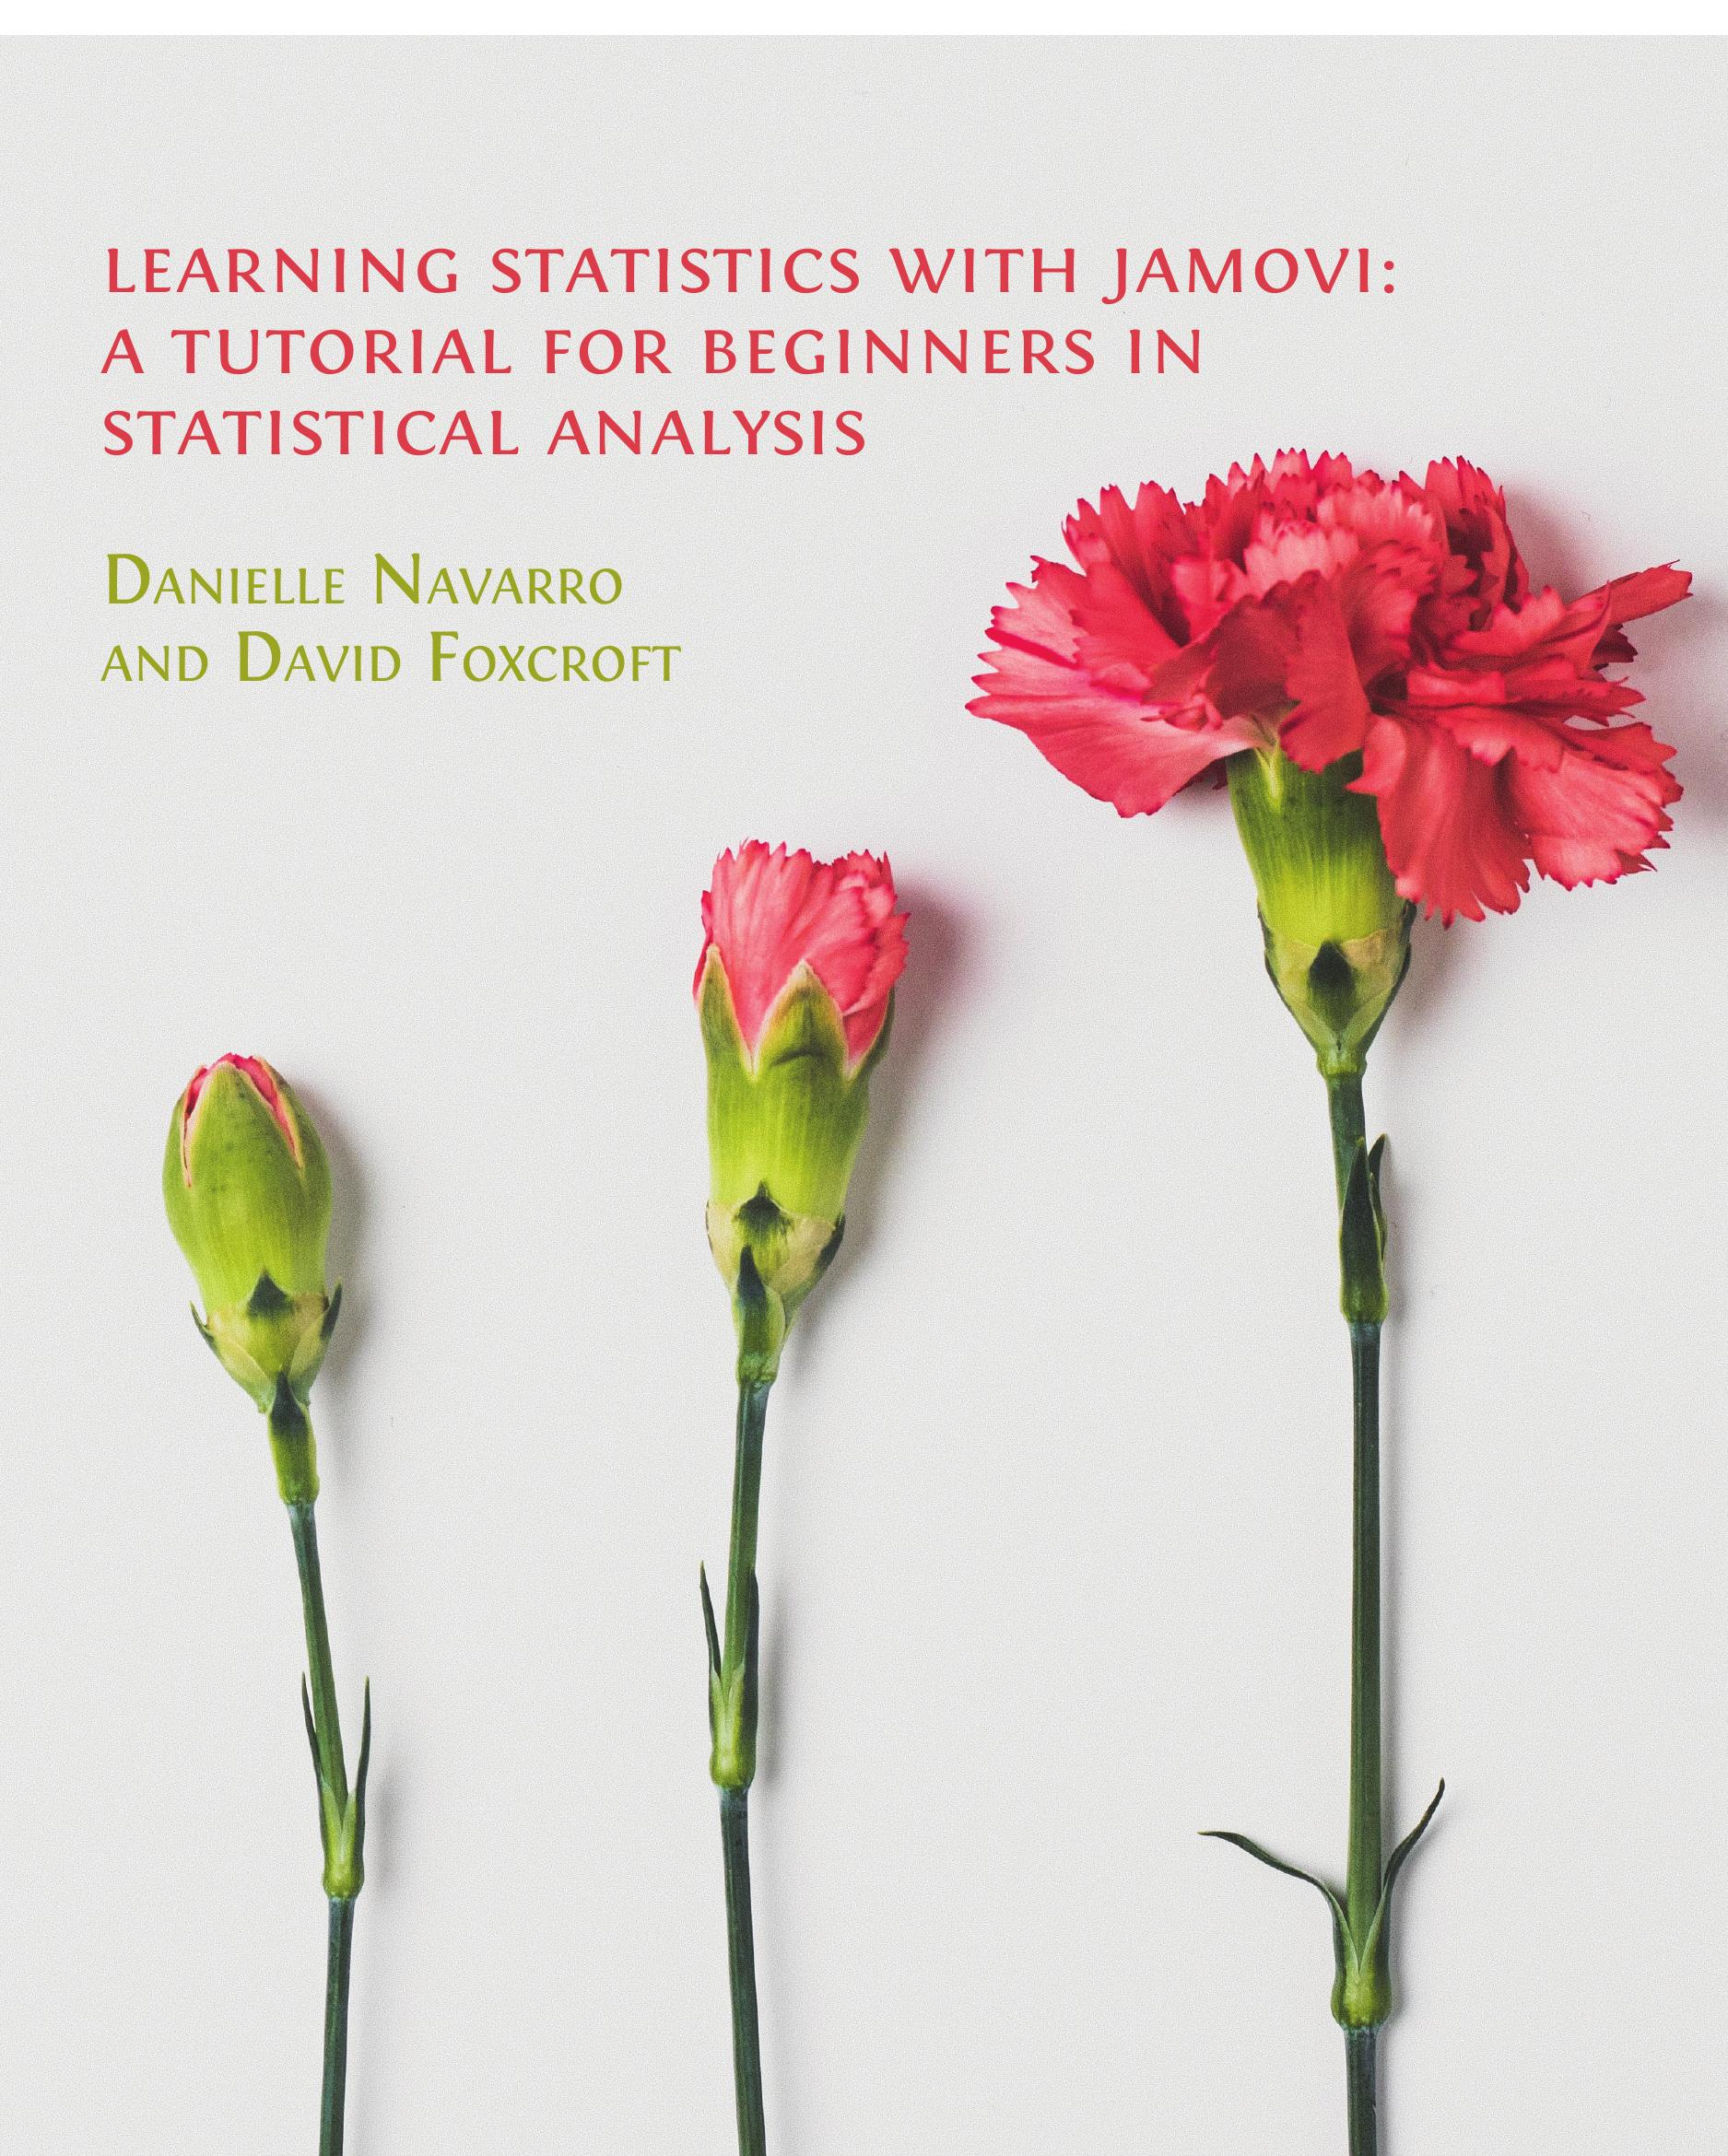
\includepdf[fitpaper=true,pages=-]{images/obp.0333}
\end{center}
\pagestyle{empty}

\let\maketitle\oldmaketitle
\maketitle

\mainmatter
\pagestyle{plain}

\let\footnote=\endnote



\pagenumbering{roman}
\hspace{0pt}
\vfill
\begin{center}

\Huge{Learning Statistics with jamovi}

\Large{A Tutorial for Beginners in Statistical Analysis}\\*[20pt]

\normalsize{Danielle Navarro and David Foxcroft}

\vfill
\end{center}
\hspace{0pt}
\pagebreak

\hspace{0pt}
\vfill

\copyright 2025 David Foxcroft and Danielle Navarro

This work is licensed under an Attribution-ShareAlike 4.0 International (CC BY-SA 4.0).

This license allows you to copy and redistribute, transform, and build upon the material for any purpose, even commercially. providing attribution is made to the authors (but not in any way that suggests that they endorse you or your use of the work). Attribution should include the following information:

Danielle Navarro and David Foxcroft, \textit{Learning statistics with jamovi: A tutorial for beginners in statistical analysis}. Cambridge, UK: Open Book Publishers, 2025, \url{https://doi.org/10.11647/OBP.0333}

Further details about CC BY-SA licenses are available at \\ \url{https://creativecommons.org/licenses/by-sa/4.0/}

All external links were active at the time of publication unless otherwise stated and have been archived via the Internet Archive Wayback Machine at \\ \url{https://archive.org/web}

Digital material and resources associated with this volume are available at \\ \url{https://doi.org/10.11647/OBP.0333\#resources}

ISBN Paperback: 978-1-80064-937-8

ISBN Hardback: 978-1-80064-938-5

ISBN Digital (PDF): 978-1-80064-939-2

DOI: 10.11647/OBP.0333


\vfill
\hspace{0pt}
\pagebreak

\hspace{0pt}
\vfill

This textbook covers the contents of an introductory statistics class, as typically taught to undergraduate psychology, health or social science students. The book covers how to get started in jamovi as well as giving an introduction to data manipulation. From a statistical perspective, the book discusses descriptive statistics and graphing first, followed by chapters on probability theory, sampling and estimation, and null hypothesis testing. After introducing the theory, the book covers the analysis of contingency tables, correlation, \textit{t}-tests, regression, ANOVA and factor analysis. Bayesian statistics are touched on at the end of the book.

Data sets used in the book are freely available for use in jamovi. All the data files you need can be accessed within jamovi via an add-on module in the jamovi library. Or you can download the files from \url{https://www.learnstatswithjamovi.com}.


Citation: Danielle Navarro and David Foxcroft, \textit{Learning statistics with jamovi: A tutorial for beginners in statistical analysis}. Cambridge, UK: Open Book Publishers, 2025, \url{https://doi.org/10.11647/OBP.0333}

\vfill
\hspace{0pt}

\ifdefined\Shaded\renewenvironment{Shaded}{\begin{tcolorbox}[frame hidden, boxrule=0pt, borderline west={3pt}{0pt}{shadecolor}, breakable, interior hidden, sharp corners, enhanced]}{\end{tcolorbox}}\fi

\renewcommand*\contentsname{Table of contents}
{
\hypersetup{linkcolor=}
\setcounter{tocdepth}{2}
\tableofcontents
}
\mainmatter
\bookmarksetup{startatroot}

\hypertarget{preface}{%
\chapter*{Preface}\label{preface}}
\addcontentsline{toc}{chapter}{Preface}

\markboth{Preface}{Preface}

This book is an adaptation of DJ Navarro (2018). Learning statistics
with R: A tutorial for psychology students and other beginners. (Version
0.6). \url{https://learningstatisticswithr.com/}.

The jamovi version of this book was first released in 2018, as version
0.65. Versions 0.70 and 0.75 were released in subsequent years with
corrections and additions; details of the changes in earlier versions of
the book can be found in the preface to version 0.75:
\url{https://github.com/user-attachments/files/18124061/learning-statistics-with-jamovi-0.75.pdf}.
In that time, many people have contacted us asking for a hard copy
version of the book. To achieve this, and to preserve the open source
attributes of the book and materials, we have worked with
\href{https://www.openbookpublishers.com/books/10.11647/obp.0333}{Open
Book Publishers} in Cambridge, UK, to release this updated version. Open
Book Publishers are the leading independent open access publisher of
academic research in the Humanities and Social Sciences in the UK. They
are award-winning, not-for-profit, run by scholars, and committed to
making high-quality research freely available to readers around the
world.

If you spot any mistakes, or have any suggestions, please do let us know
by raising an issue at
\url{https://github.com/davidfoxcroft/lsj-book/issues}.

\emph{David Foxcroft\\
January 1st, 2025}

\part{Beginnings}

\hypertarget{sec-Correlation-and-linear-regression}{%
\chapter{Correlation and linear
regression}\label{sec-Correlation-and-linear-regression}}

\placetextbox{0.26}{0.06}{\scriptsize{©2025 D. Foxcroft and D. Navarro,}}
\placetextbox{0.205}{0.05}{\scriptsize{CC BY-SA 4.0}}
\placetextbox{0.70}{0.06}{\scriptsize{\url{https://doi.org/10.11647/OBP.0333/12}}}

The goal in this chapter is to introduce \textbf{correlation} and
\textbf{linear regression}. These are the standard tools that
statisticians rely on when analysing the relationship between continuous
predictors and continuous outcomes.

\hypertarget{correlations}{%
\section{Correlations}\label{correlations}}

In this section we'll talk about how to describe the relationships
between variables in the data. To do that, we want to talk mostly about
the \textbf{correlation} between variables. But first, we need some data
(Table~\ref{tbl-tab12-1}).

\hypertarget{the-data}{%
\subsection{The data}\label{the-data}}

\hypertarget{tbl-tab12-1}{}
 
  \providecommand{\huxb}[2]{\arrayrulecolor[RGB]{#1}\global\arrayrulewidth=#2pt}
  \providecommand{\huxvb}[2]{\color[RGB]{#1}\vrule width #2pt}
  \providecommand{\huxtpad}[1]{\rule{0pt}{#1}}
  \providecommand{\huxbpad}[1]{\rule[-#1]{0pt}{#1}}

\begin{table}[ht]
\caption{\label{tbl-tab12-1}Data for correlation analysis -- descriptive statistics for the
\emph{parenthood} data }\tabularnewline

\begin{centerbox}
\begin{threeparttable}
\setlength{\tabcolsep}{0pt}
\begin{tabularx}{0.9\textwidth}{p{0.18\textwidth} p{0.128571428571429\textwidth} p{0.128571428571429\textwidth} p{0.128571428571429\textwidth} p{0.128571428571429\textwidth} p{0.128571428571429\textwidth} p{0.128571428571429\textwidth}}


\hhline{>{\huxb{0, 0, 0}{0.4}}->{\huxb{0, 0, 0}{0.4}}->{\huxb{0, 0, 0}{0.4}}->{\huxb{0, 0, 0}{0.4}}->{\huxb{0, 0, 0}{0.4}}->{\huxb{0, 0, 0}{0.4}}->{\huxb{0, 0, 0}{0.4}}-}
\arrayrulecolor{black}

\multicolumn{1}{!{\huxvb{0, 0, 0}{0}}p{0.18\textwidth}!{\huxvb{0, 0, 0}{0}}}{\hspace{0pt}\parbox[b]{0.18\textwidth-0pt-12pt}{\huxtpad{2pt + 1em}\centering \textbf{variable}\huxbpad{2pt}}} &
\multicolumn{1}{p{0.128571428571429\textwidth}!{\huxvb{0, 0, 0}{0}}}{\hspace{12pt}\parbox[b]{0.128571428571429\textwidth-12pt-12pt}{\huxtpad{2pt + 1em}\centering \textbf{min}\huxbpad{2pt}}} &
\multicolumn{1}{p{0.128571428571429\textwidth}!{\huxvb{0, 0, 0}{0}}}{\hspace{12pt}\parbox[b]{0.128571428571429\textwidth-12pt-12pt}{\huxtpad{2pt + 1em}\centering \textbf{max}\huxbpad{2pt}}} &
\multicolumn{1}{p{0.128571428571429\textwidth}!{\huxvb{0, 0, 0}{0}}}{\hspace{12pt}\parbox[b]{0.128571428571429\textwidth-12pt-12pt}{\huxtpad{2pt + 1em}\centering \textbf{mean}\huxbpad{2pt}}} &
\multicolumn{1}{p{0.128571428571429\textwidth}!{\huxvb{0, 0, 0}{0}}}{\hspace{12pt}\parbox[b]{0.128571428571429\textwidth-12pt-12pt}{\huxtpad{2pt + 1em}\centering \textbf{median}\huxbpad{2pt}}} &
\multicolumn{1}{p{0.128571428571429\textwidth}!{\huxvb{0, 0, 0}{0}}}{\hspace{12pt}\parbox[b]{0.128571428571429\textwidth-12pt-12pt}{\huxtpad{2pt + 1em}\centering \textbf{std. dev}\huxbpad{2pt}}} &
\multicolumn{1}{p{0.128571428571429\textwidth}!{\huxvb{0, 0, 0}{0}}}{\hspace{12pt}\parbox[b]{0.128571428571429\textwidth-12pt-0pt}{\huxtpad{2pt + 1em}\centering \textbf{IQR}\huxbpad{2pt}}} \tabularnewline[-0.5pt]


\hhline{>{\huxb{0, 0, 0}{0.4}}->{\huxb{0, 0, 0}{0.4}}->{\huxb{0, 0, 0}{0.4}}->{\huxb{0, 0, 0}{0.4}}->{\huxb{0, 0, 0}{0.4}}->{\huxb{0, 0, 0}{0.4}}->{\huxb{0, 0, 0}{0.4}}-}
\arrayrulecolor{black}

\multicolumn{1}{!{\huxvb{0, 0, 0}{0}}p{0.18\textwidth}!{\huxvb{0, 0, 0}{0}}}{\hspace{0pt}\parbox[b]{0.18\textwidth-0pt-12pt}{\huxtpad{2pt + 1em}\centering Dani's grumpiness\huxbpad{2pt}}} &
\multicolumn{1}{p{0.128571428571429\textwidth}!{\huxvb{0, 0, 0}{0}}}{\hspace{12pt}\parbox[b]{0.128571428571429\textwidth-12pt-12pt}{\huxtpad{2pt + 1em}\centering 41\huxbpad{2pt}}} &
\multicolumn{1}{p{0.128571428571429\textwidth}!{\huxvb{0, 0, 0}{0}}}{\hspace{12pt}\parbox[b]{0.128571428571429\textwidth-12pt-12pt}{\huxtpad{2pt + 1em}\centering 91\huxbpad{2pt}}} &
\multicolumn{1}{p{0.128571428571429\textwidth}!{\huxvb{0, 0, 0}{0}}}{\hspace{12pt}\parbox[b]{0.128571428571429\textwidth-12pt-12pt}{\huxtpad{2pt + 1em}\centering 63.71\huxbpad{2pt}}} &
\multicolumn{1}{p{0.128571428571429\textwidth}!{\huxvb{0, 0, 0}{0}}}{\hspace{12pt}\parbox[b]{0.128571428571429\textwidth-12pt-12pt}{\huxtpad{2pt + 1em}\centering 62\huxbpad{2pt}}} &
\multicolumn{1}{p{0.128571428571429\textwidth}!{\huxvb{0, 0, 0}{0}}}{\hspace{12pt}\parbox[b]{0.128571428571429\textwidth-12pt-12pt}{\huxtpad{2pt + 1em}\centering 10.05\huxbpad{2pt}}} &
\multicolumn{1}{p{0.128571428571429\textwidth}!{\huxvb{0, 0, 0}{0}}}{\hspace{12pt}\parbox[b]{0.128571428571429\textwidth-12pt-0pt}{\huxtpad{2pt + 1em}\centering 14\huxbpad{2pt}}} \tabularnewline[-0.5pt]


\hhline{}
\arrayrulecolor{black}

\multicolumn{1}{!{\huxvb{0, 0, 0}{0}}p{0.18\textwidth}!{\huxvb{0, 0, 0}{0}}}{\hspace{0pt}\parbox[b]{0.18\textwidth-0pt-12pt}{\huxtpad{2pt + 1em}\centering Dani's hours slept\huxbpad{2pt}}} &
\multicolumn{1}{p{0.128571428571429\textwidth}!{\huxvb{0, 0, 0}{0}}}{\hspace{12pt}\parbox[b]{0.128571428571429\textwidth-12pt-12pt}{\huxtpad{2pt + 1em}\centering 4.84\huxbpad{2pt}}} &
\multicolumn{1}{p{0.128571428571429\textwidth}!{\huxvb{0, 0, 0}{0}}}{\hspace{12pt}\parbox[b]{0.128571428571429\textwidth-12pt-12pt}{\huxtpad{2pt + 1em}\centering 9.00\huxbpad{2pt}}} &
\multicolumn{1}{p{0.128571428571429\textwidth}!{\huxvb{0, 0, 0}{0}}}{\hspace{12pt}\parbox[b]{0.128571428571429\textwidth-12pt-12pt}{\huxtpad{2pt + 1em}\centering 6.97\huxbpad{2pt}}} &
\multicolumn{1}{p{0.128571428571429\textwidth}!{\huxvb{0, 0, 0}{0}}}{\hspace{12pt}\parbox[b]{0.128571428571429\textwidth-12pt-12pt}{\huxtpad{2pt + 1em}\centering 7.03\huxbpad{2pt}}} &
\multicolumn{1}{p{0.128571428571429\textwidth}!{\huxvb{0, 0, 0}{0}}}{\hspace{12pt}\parbox[b]{0.128571428571429\textwidth-12pt-12pt}{\huxtpad{2pt + 1em}\centering 1.02\huxbpad{2pt}}} &
\multicolumn{1}{p{0.128571428571429\textwidth}!{\huxvb{0, 0, 0}{0}}}{\hspace{12pt}\parbox[b]{0.128571428571429\textwidth-12pt-0pt}{\huxtpad{2pt + 1em}\centering 1.45\huxbpad{2pt}}} \tabularnewline[-0.5pt]


\hhline{}
\arrayrulecolor{black}

\multicolumn{1}{!{\huxvb{0, 0, 0}{0}}p{0.18\textwidth}!{\huxvb{0, 0, 0}{0}}}{\hspace{0pt}\parbox[b]{0.18\textwidth-0pt-12pt}{\huxtpad{2pt + 1em}\centering Dani's son's hours slept\huxbpad{2pt}}} &
\multicolumn{1}{p{0.128571428571429\textwidth}!{\huxvb{0, 0, 0}{0}}}{\hspace{12pt}\parbox[b]{0.128571428571429\textwidth-12pt-12pt}{\huxtpad{2pt + 1em}\centering 3.25\huxbpad{2pt}}} &
\multicolumn{1}{p{0.128571428571429\textwidth}!{\huxvb{0, 0, 0}{0}}}{\hspace{12pt}\parbox[b]{0.128571428571429\textwidth-12pt-12pt}{\huxtpad{2pt + 1em}\centering 12.07\huxbpad{2pt}}} &
\multicolumn{1}{p{0.128571428571429\textwidth}!{\huxvb{0, 0, 0}{0}}}{\hspace{12pt}\parbox[b]{0.128571428571429\textwidth-12pt-12pt}{\huxtpad{2pt + 1em}\centering 8.05\huxbpad{2pt}}} &
\multicolumn{1}{p{0.128571428571429\textwidth}!{\huxvb{0, 0, 0}{0}}}{\hspace{12pt}\parbox[b]{0.128571428571429\textwidth-12pt-12pt}{\huxtpad{2pt + 1em}\centering 7.95\huxbpad{2pt}}} &
\multicolumn{1}{p{0.128571428571429\textwidth}!{\huxvb{0, 0, 0}{0}}}{\hspace{12pt}\parbox[b]{0.128571428571429\textwidth-12pt-12pt}{\huxtpad{2pt + 1em}\centering 2.07\huxbpad{2pt}}} &
\multicolumn{1}{p{0.128571428571429\textwidth}!{\huxvb{0, 0, 0}{0}}}{\hspace{12pt}\parbox[b]{0.128571428571429\textwidth-12pt-0pt}{\huxtpad{2pt + 1em}\centering 3.21\huxbpad{2pt}}} \tabularnewline[-0.5pt]


\hhline{>{\huxb{0, 0, 0}{0.4}}->{\huxb{0, 0, 0}{0.4}}->{\huxb{0, 0, 0}{0.4}}->{\huxb{0, 0, 0}{0.4}}->{\huxb{0, 0, 0}{0.4}}->{\huxb{0, 0, 0}{0.4}}->{\huxb{0, 0, 0}{0.4}}-}
\arrayrulecolor{black}
\end{tabularx} 

\end{threeparttable}\par\end{centerbox}

\end{table}
 

Let's turn to a topic close to every parent's heart: sleep. The data set
we'll use is fictitious, but based on real events. Suppose I'm curious
to find out how much my infant son's sleeping habits affect my mood.
Let's say that I can rate my grumpiness very precisely, on a scale from
0 (not at all grumpy) to \(100\) (grumpy as a very, very grumpy old man
or woman). And lets also assume that I've been measuring my grumpiness,
my sleeping patterns and my son's sleeping patterns for quite some time
now. Let's say, for \(100\) days. And, being a nerd, I've saved the data
as a file called \emph{parenthood.csv}. If we load the data we can see
that the file contains four variables dani.sleep, baby.sleep, dani.grump
and day. Note that when you first load this data set jamovi may not have
guessed the data type for each variable correctly, in which case you
should fix it: dani.sleep, baby.sleep, dani.grump and day can be
specified as continuous variables, and ID is a nominal(integer)
variable.\footnote{I've noticed that in jamovi you can also specify an
  `ID' variable type, but for our purposes it does not matter how we
  specify the ID variable as we won't be including it in any analyses.}

Next, I'll take a look at some basic descriptive statistics and, to give
a graphical depiction of what each of the three interesting variables
looks like, Figure~\ref{fig-fig12-1} plots histograms. One thing to
note: just because jamovi can calculate dozens of different statistics
doesn't mean you should report all of them. If I were writing this up
for a report, I'd probably pick out those statistics that are of most
interest to me (and to my readership), and then put them into a nice,
simple table like the one in Table 12.1.\footnote{Actually, even that
  table is more than I'd bother with. In practice most people pick one
  measure of central tendency, and one measure of variability only.}
Notice that when I put it into a table, I gave everything ``human
readable'' names. This is always good practice. Notice also that I'm not
getting enough sleep. This isn't good practice, but other parents tell
me that it's pretty standard.

\begin{figure}

\begin{minipage}[b]{0.33\linewidth}

{\centering 

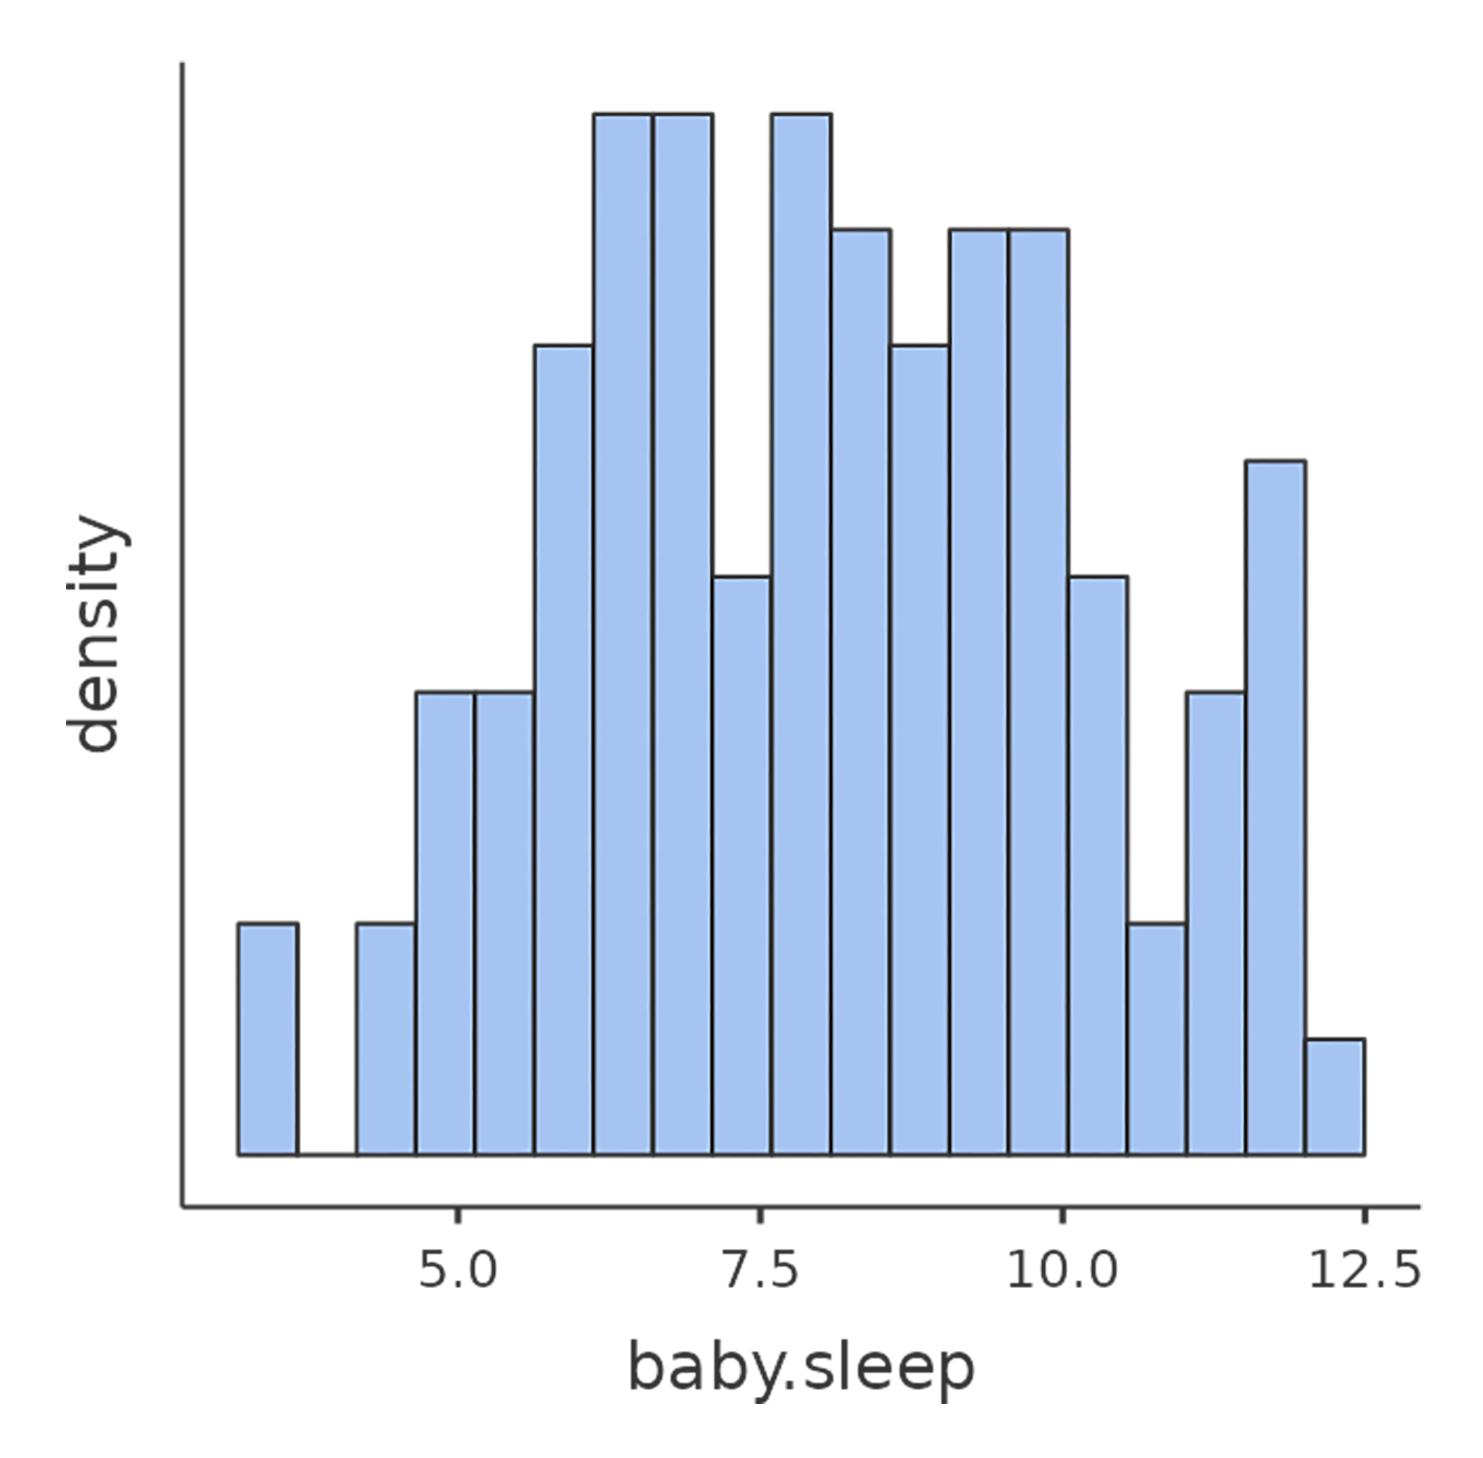
\includegraphics{images/fig12-1a.png}

}

\subcaption{\label{fig-fig12-1a}}
\end{minipage}%
%
\begin{minipage}[b]{0.33\linewidth}

{\centering 

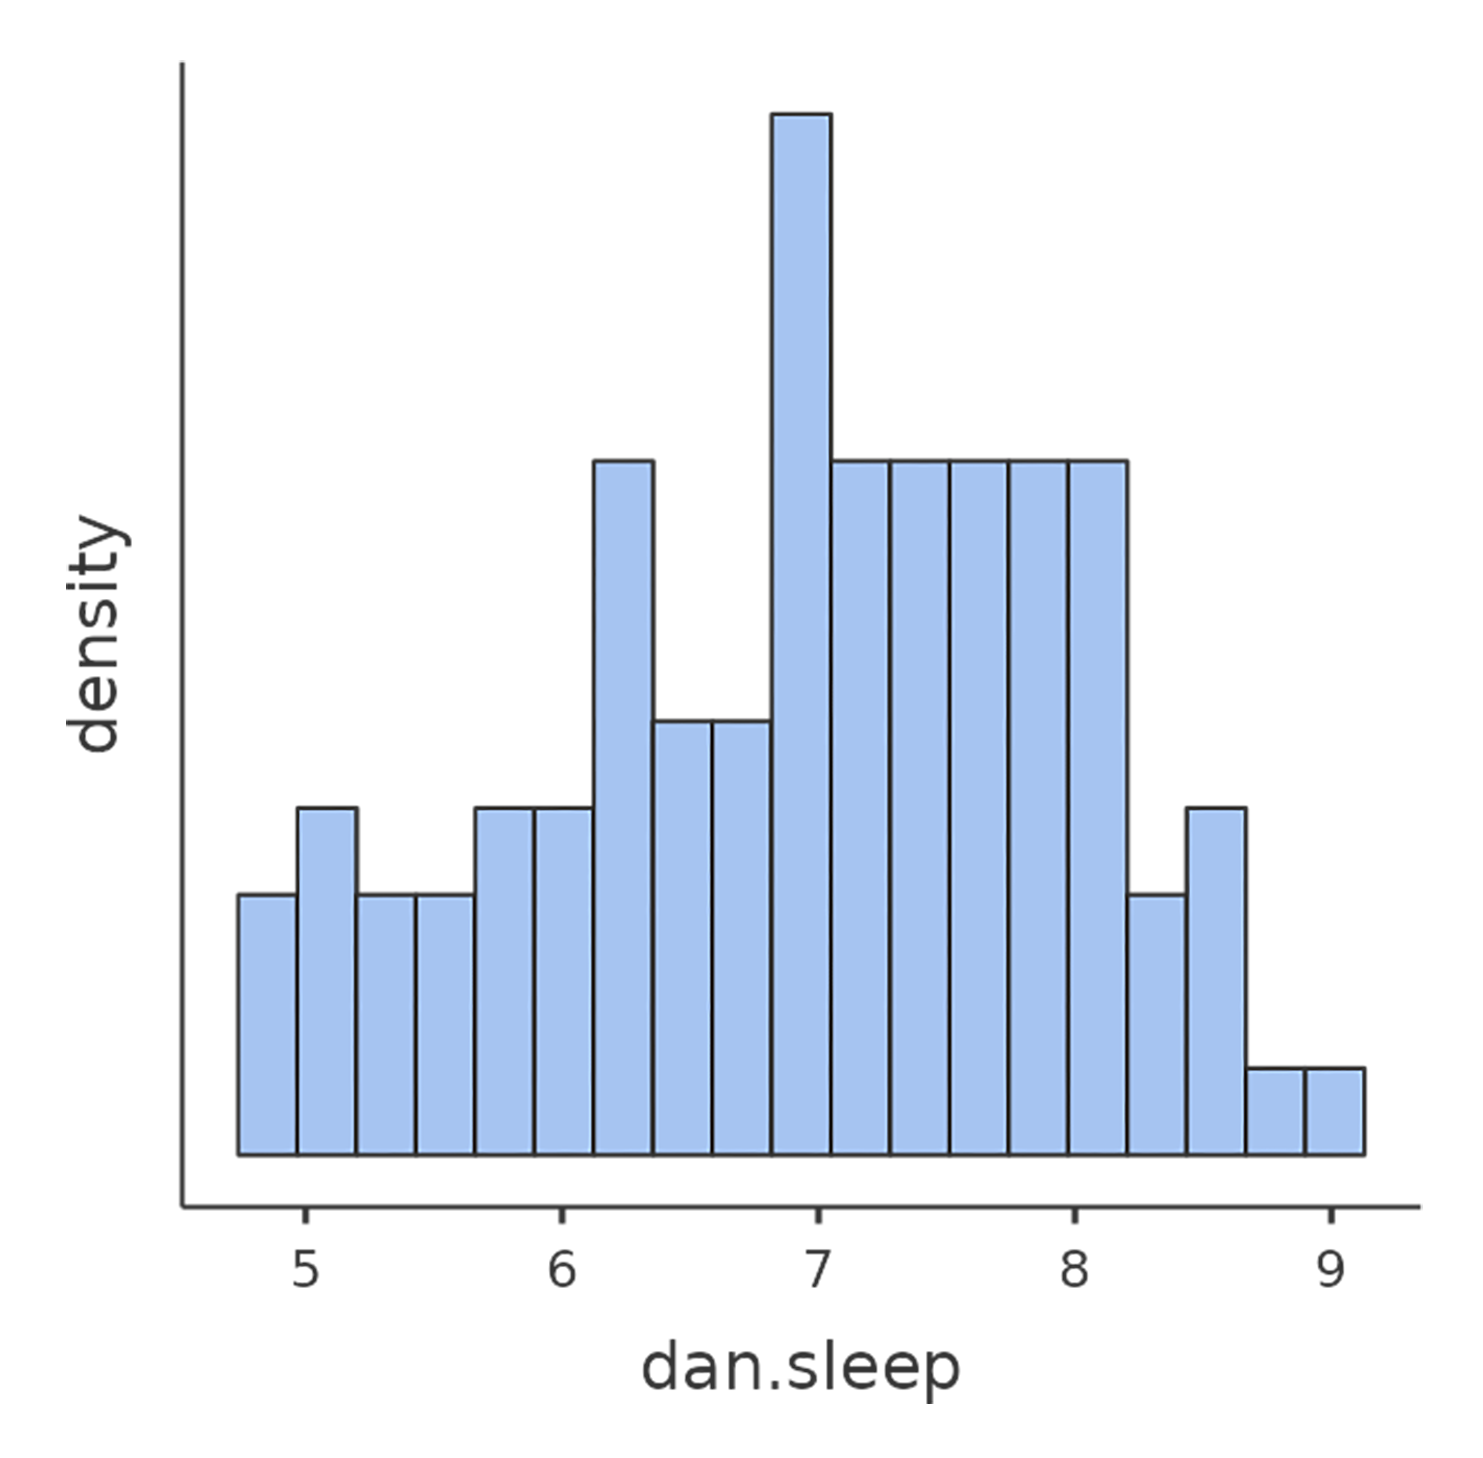
\includegraphics{images/fig12-1b.png}

}

\subcaption{\label{fig-fig12-1b}}
\end{minipage}%
%
\begin{minipage}[b]{0.33\linewidth}

{\centering 

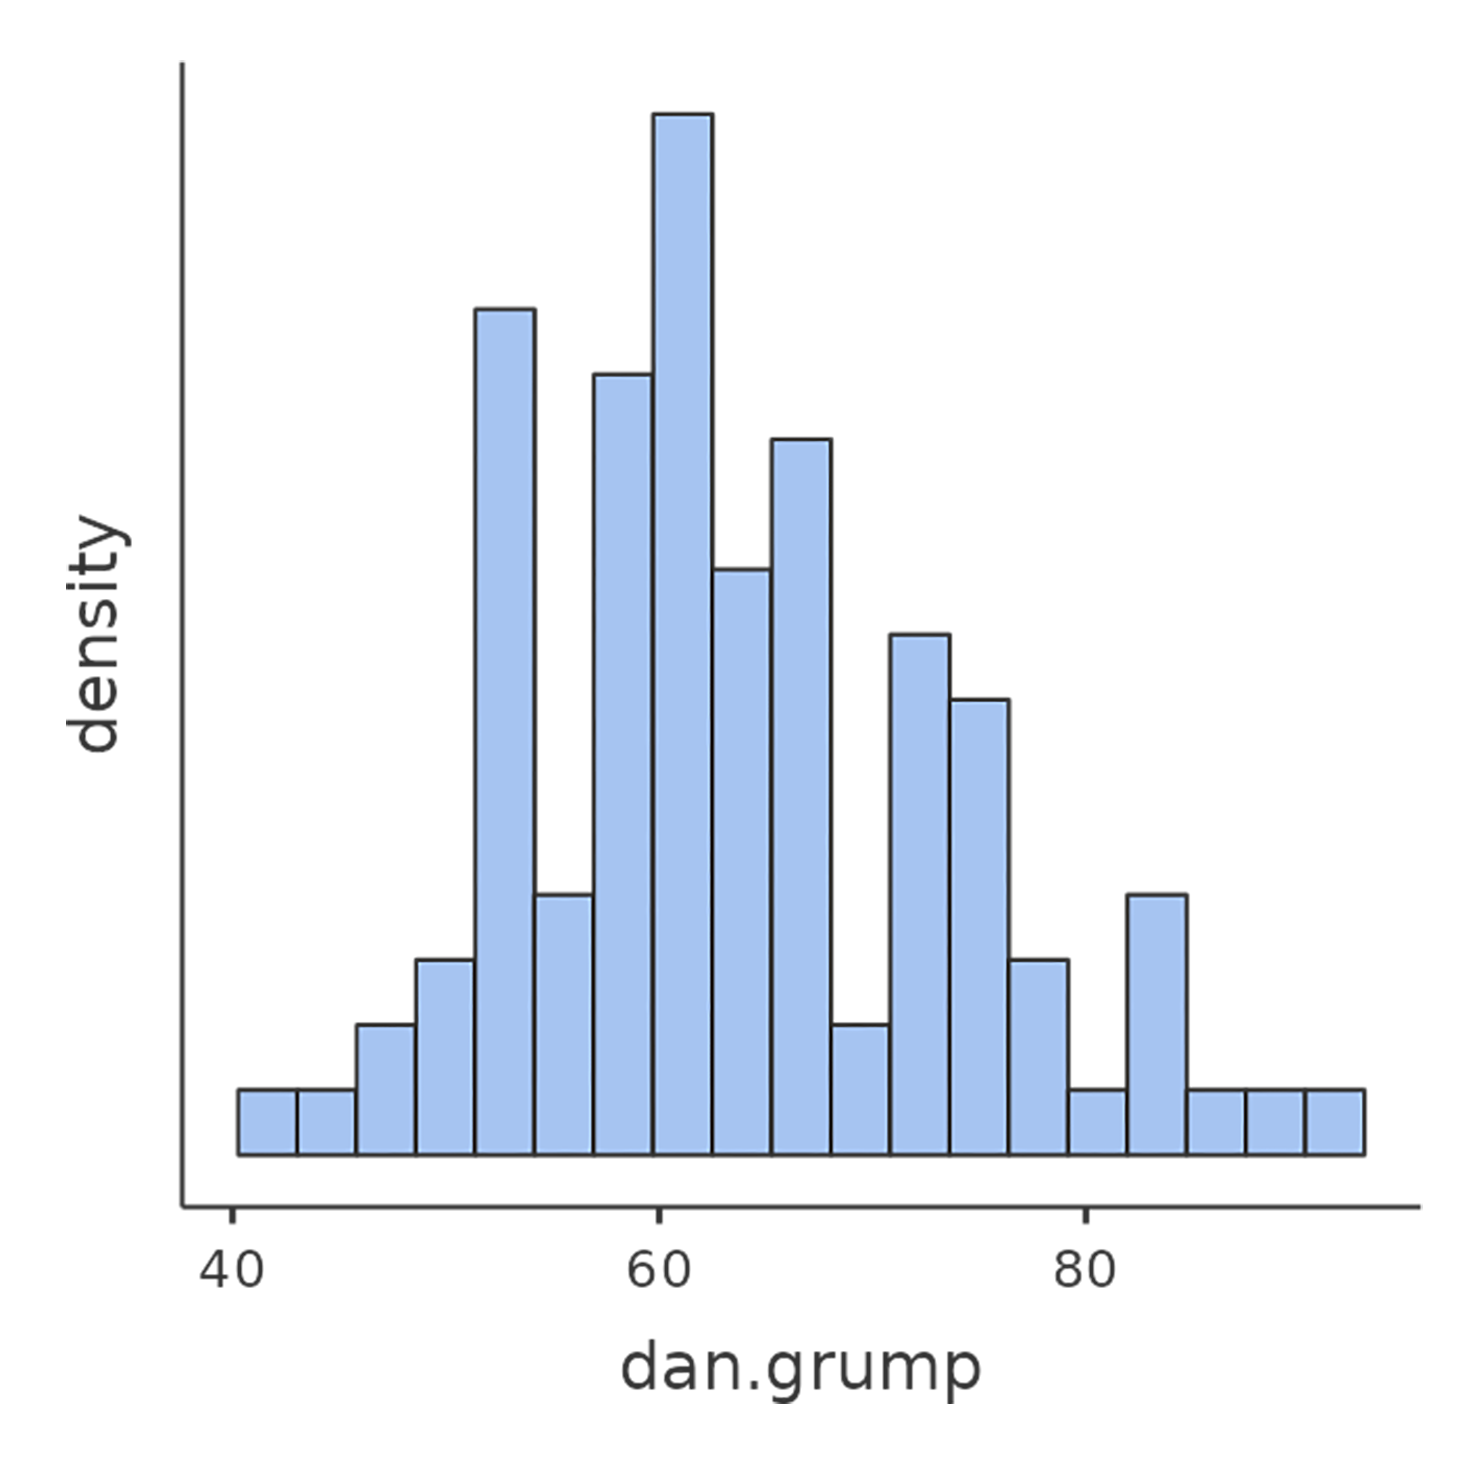
\includegraphics{images/fig12-1c.png}

}

\subcaption{\label{fig-fig12-1c}}
\end{minipage}%

\caption{\label{fig-fig12-1}Histograms from jamovi for the three
interesting variables in the \emph{parenthood} data set}

\end{figure}

\hypertarget{the-strength-and-direction-of-a-relationship}{%
\subsection{The strength and direction of a
relationship}\label{the-strength-and-direction-of-a-relationship}}

We can draw scatterplots to give us a general sense of how closely
related two variables are. Ideally though, we might want to say a bit
more about it than that. For instance, let's compare the relationship
between baby.sleep and dani.grump (Figure~\ref{fig-fig12-2a}), left,
with that between dani.sleep and dani.grump (Figure~\ref{fig-fig12-2b}),
right. When looking at these two plots side by side, it's clear that the
relationship is qualitatively the same in both cases: more sleep equals
less grump! However, it's also pretty obvious that the relationship
between dani.sleep and dani.grump is stronger than the relationship
between baby.sleep and dani.grump. The plot on the right is ``neater''
than the one on the left. What it feels like is that if you want to
predict what my mood is, it'd help you a little bit to know how many
hours my son slept, but it'd be more helpful to know how many hours I
slept.

\begin{figure}[H]

\begin{minipage}[b]{0.50\linewidth}

{\centering 


\includegraphics{images/fig12-2a.png}

}

\subcaption{\label{fig-fig12-2a}}
\end{minipage}%
%
\begin{minipage}[b]{0.50\linewidth}

{\centering 


\includegraphics{images/fig12-2b.png}

}

\subcaption{\label{fig-fig12-2b}}
\end{minipage}%

\caption{\label{fig-fig12-2}Scatterplots from jamovi showing the
relationship between baby.sleep and dani.grump (left) and the
relationship between dani.sleep and dani.grump (right)}

\end{figure}

In contrast, let's consider the two scatterplots shown in
Figure~\ref{fig-fig12-3}. If we compare the scatterplot of ``baby.sleep
v dani.grump'' (left) to the scatterplot of ``baby.sleep v dani.sleep''
(right), the overall strength of the relationship is the same, but the
direction is different. That is, if my son sleeps more, I get more sleep
(positive relationship, right-hand side), but if he sleeps more then I
get less grumpy (negative relationship, left-hand side).

\begin{figure}[h!]

\begin{minipage}[b]{0.50\linewidth}

{\centering 


\includegraphics{images/fig12-2a.png}

}

\subcaption{\label{fig-fig12-3a}}
\end{minipage}%
%
\begin{minipage}[b]{0.50\linewidth}

{\centering 


\includegraphics{images/fig12-3b.png}

}

\subcaption{\label{fig-fig12-3b}}
\end{minipage}%

\caption{\label{fig-fig12-3}Scatterplots from jamovi showing the
relationship between baby.sleep and dani.grump (left), as compared to
the relationship between baby.sleep and dani.sleep (right)}

\end{figure}

\hypertarget{the-correlation-coefficient}{%
\subsection{The correlation
coefficient}\label{the-correlation-coefficient}}

We can make these ideas a bit more explicit by introducing the idea of a
\textbf{correlation coefficient} (or, more specifically, Pearson's
correlation coefficient), which is traditionally denoted as r. The
correlation coefficient between two variables \(X\) and \(Y\) (sometimes
denoted \(r_{XY}\) ), which we'll define more precisely in the next
section, is a measure that varies from -1 to 1. When \(r = -1\) it means
that we have a perfect negative relationship, and when \(r = 1\) it
means we have a perfect positive relationship. When \(r = 0\), there's
no relationship at all. If you look at Figure~\ref{fig-fig12-4}, you can
see several plots showing what different correlations look like.

{[}Additional technical detail\footnote{The formula for the Pearson's
  correlation coefficient can be written in several different ways. I
  think the simplest way to write down the formula is to break it into
  two steps. Firstly, let's introduce the idea of a \textbf{covariance}.
  The covariance between two variables \(X\) and \(Y\) is a
  generalisation of the notion of the variance and is a mathematically
  simple way of describing the relationship between two variables that
  isn't terribly informative to humans:
  \[Cov(X,Y)=\frac{1}{N-1}\sum_{i=1}^N(X_i-\bar{X})(Y_i-\bar{Y})\]
  Because we're multiplying (i.e., taking the ``product'' of) a quantity
  that depends on X by a quantity that depends on Y and then
  averaging,\(^a\) you can think of the formula for the covariance as an
  ``average cross product'' between \(X\) and \(Y\). The covariance has
  the nice property that, if \(X\) and \(Y\) are entirely unrelated,
  then the covariance is exactly zero. If the relationship between them
  is positive (in the sense shown in Figure~\ref{fig-fig12-4} then the
  covariance is also positive, and if the relationship is negative then
  the covariance is also negative. In other words, the covariance
  captures the basic qualitative idea of correlation. Unfortunately, the
  raw magnitude of the covariance isn't easy to interpret as it depends
  on the units in which \(X\) and \(Y\) are expressed and, worse yet,
  the actual units that the covariance itself is expressed in are really
  weird. For instance, if \(X\) refers to the dani.sleep variable
  (units: hours) and \(Y\) refers to the dani.grump variable (units:
  grumps), then the units for their covariance are
  \(hours \times grumps\). And I have no freaking idea what that would
  even mean. The Pearson correlation coefficient r fixes this
  interpretation problem by standardising the covariance, in pretty much
  the exact same way that the \emph{z}-score standardises a raw score,
  by dividing by the standard deviation. However, because we have two
  variables that contribute to the covariance, the standardisation only
  works if we divide by both standard deviations.\(^b\) In other words,
  the correlation between \(X\) and \(Y\) can be written as follows:
  \[r_{XY}=\frac{Cov(X,Y)}{\hat{\sigma}_X\hat{\sigma}_Y}\]---\(^a\) Just
  like we saw with the variance and the standard deviation, in practice
  we divide by \(N - 1\) rather than \(N\). \(^b\) This is an
  oversimplification, but it'll do for our purposes.}{]}

\begin{figure}[h!]

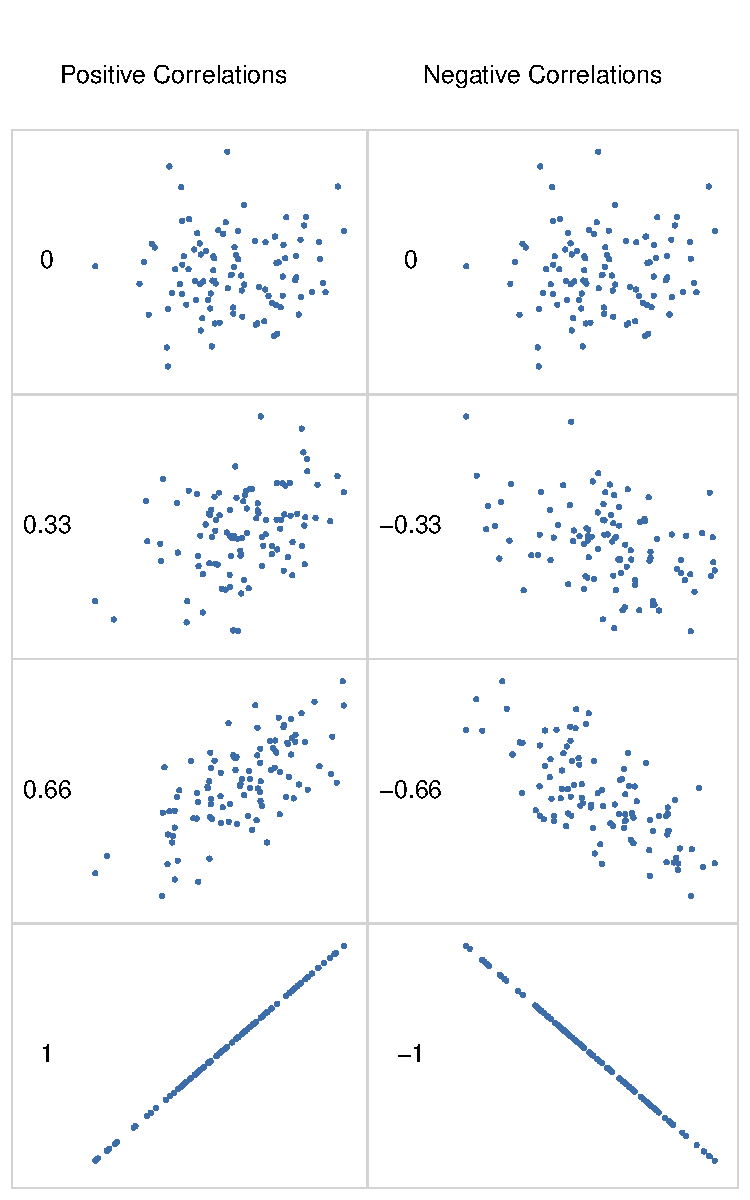
\includegraphics[width=1\textwidth,height=\textheight]{12-Correlation-and-linear-regression_files/figure-pdf/fig-fig12-4-1.pdf} \hfill{}

\caption{\label{fig-fig12-4}Illustration of the effect of varying the
strength and direction of a correlation. In the left-hand column, the
correlations are \(0, .33, .66\) and \(1\). In the right-hand column,
the correlations are \(0, -.33, -.66\) and \(-1\)}

\end{figure}

By standardising the covariance, not only do we keep all of the nice
properties of the covariance discussed earlier, but the actual values of
r are on a meaningful scale: r = 1 implies a perfect positive
relationship and \(r = -1\) implies a perfect negative relationship.
I'll expand a little more on this point later, in the section on
\protect\hyperlink{interpreting-a-correlation}{Interpreting a
correlation}. But before I do, let's look at how to calculate
correlations in jamovi.

\hypertarget{calculating-correlations-in-jamovi}{%
\subsection{Calculating correlations in
jamovi}\label{calculating-correlations-in-jamovi}}

Calculating correlations in jamovi can be done by clicking on the
`Regression' -- `Correlation Matrix' button. Transfer all four
continuous variables across into the box on the right to get the output
in Figure~\ref{fig-fig12-5}.

\begin{figure}[h!]

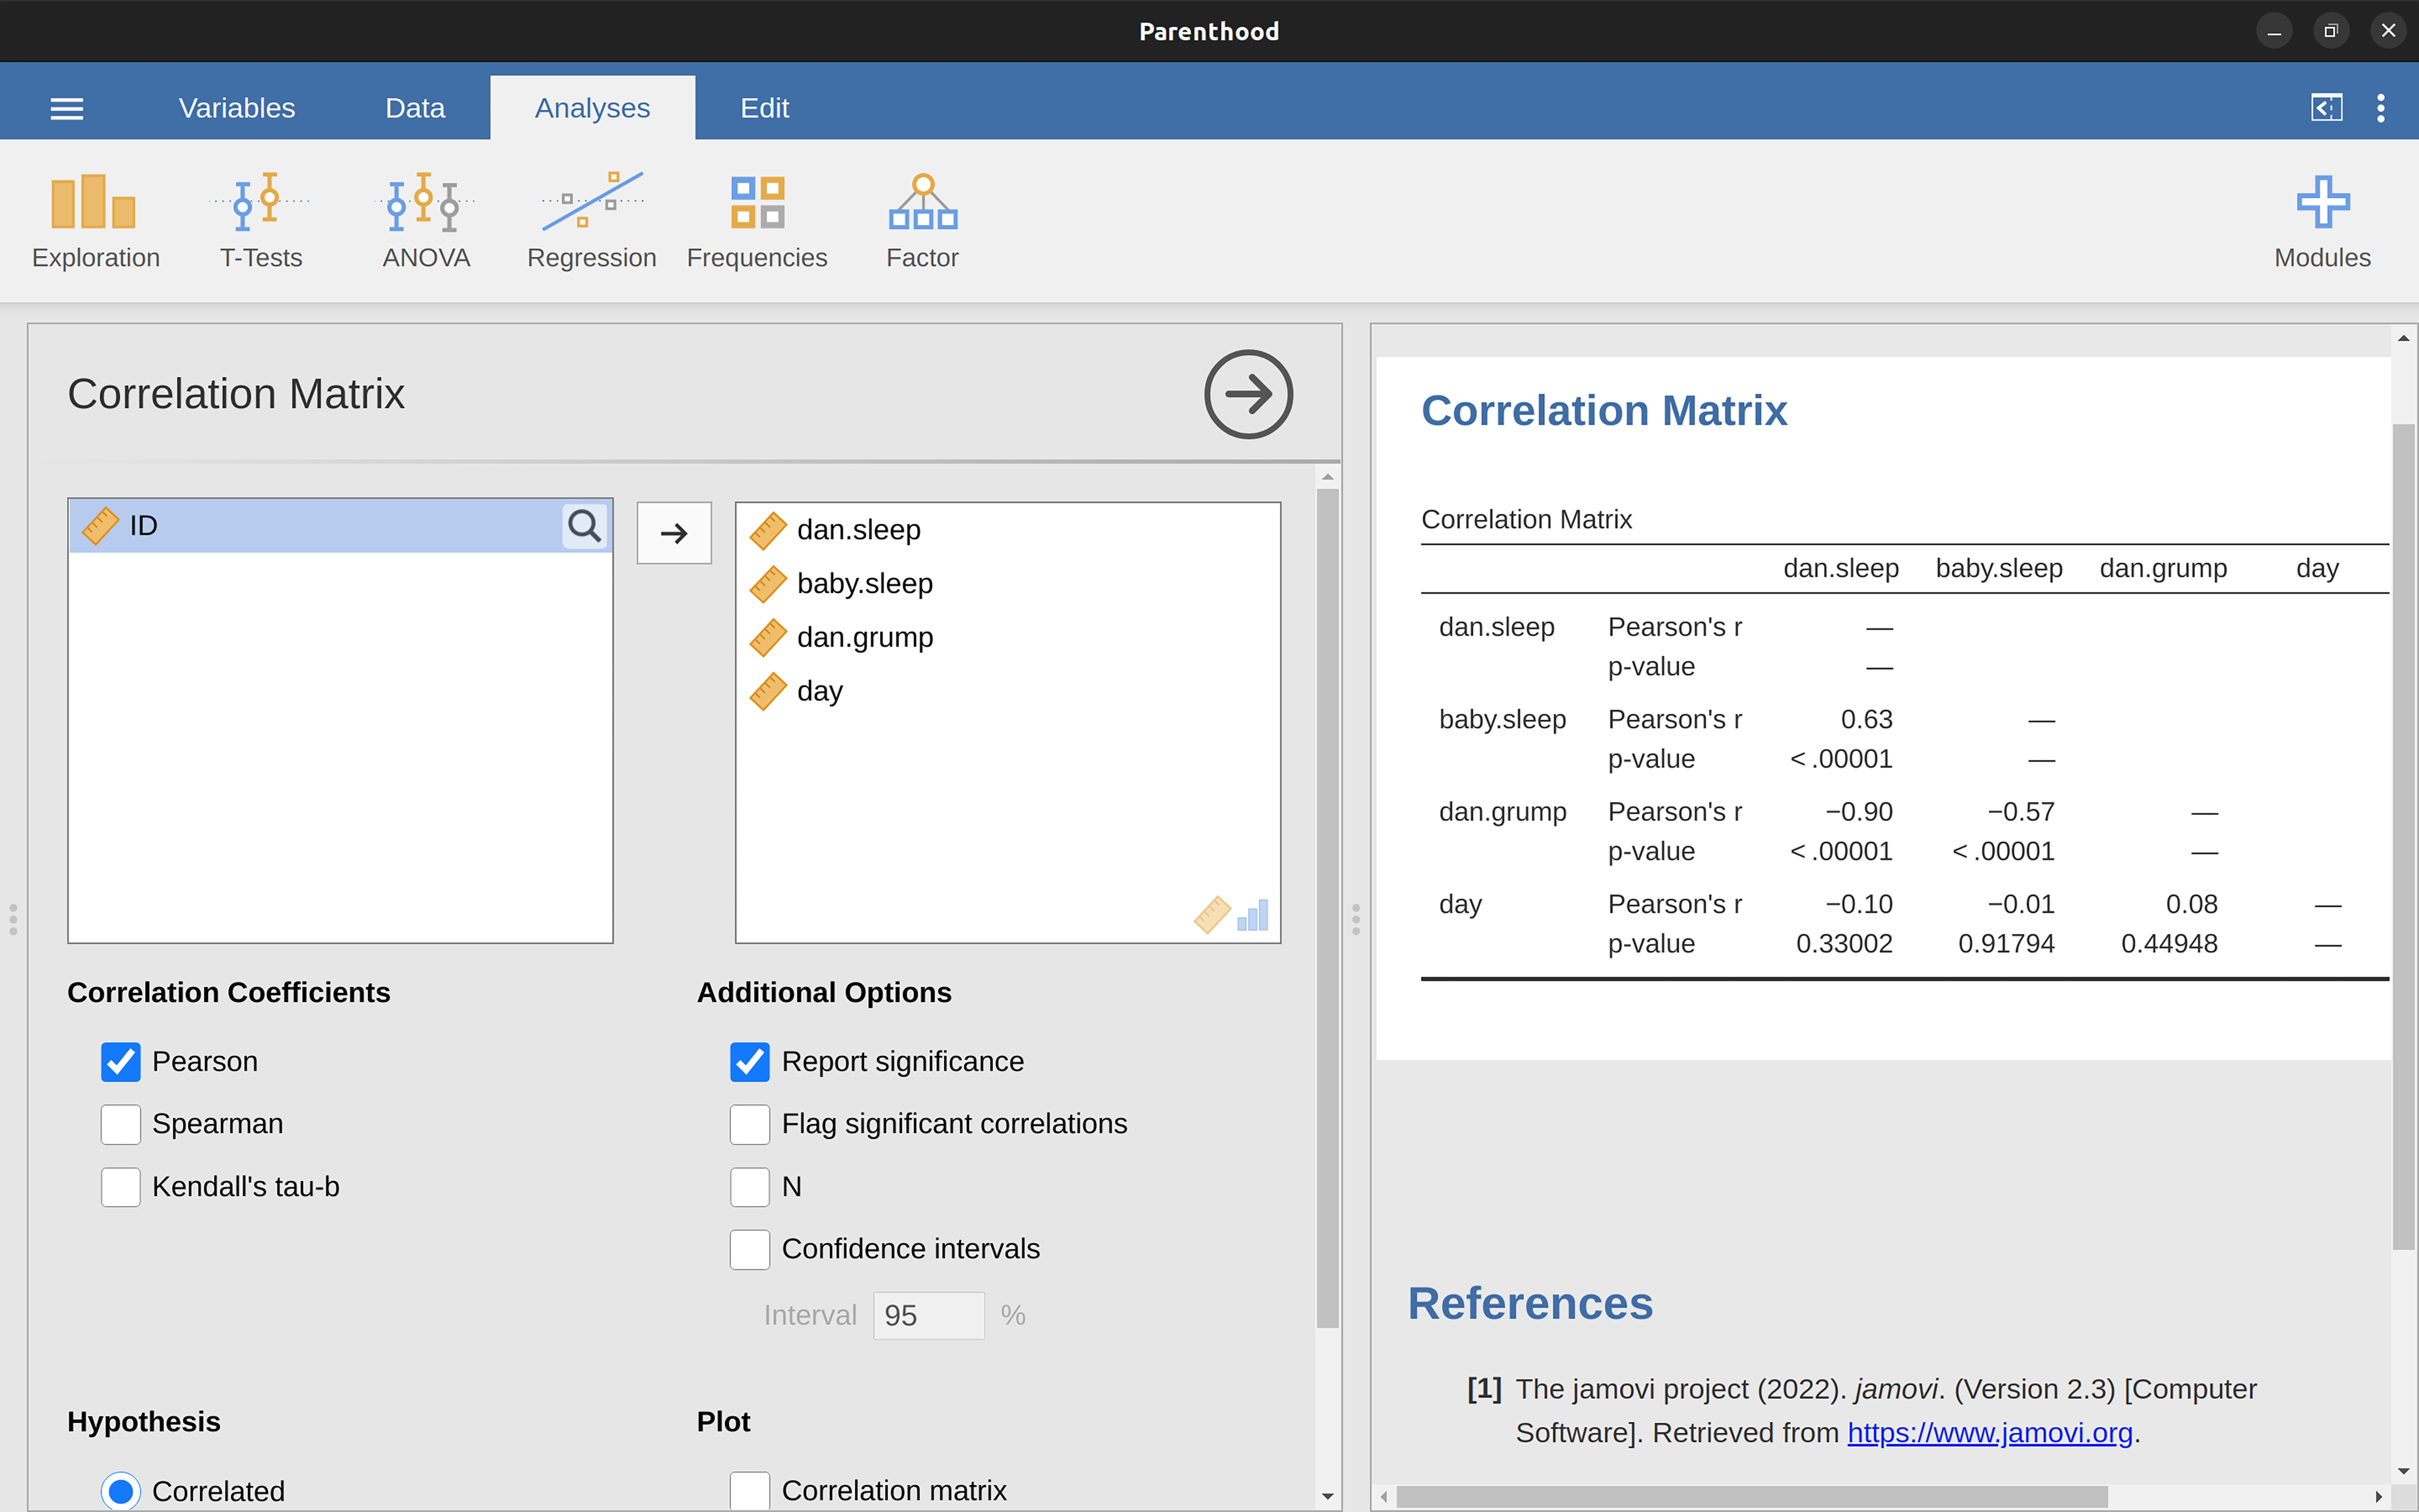
\includegraphics[width=0.9\textwidth,height=\textheight]{images/fig12-5.png} \hfill{}

\caption{\label{fig-fig12-5}Correlations between variables in the
\emph{parenthood.csv} file}

\end{figure}

\hypertarget{interpreting-a-correlation}{%
\subsection{Interpreting a
correlation}\label{interpreting-a-correlation}}

Naturally, in real life you don't see many correlations of \(1\). So how
should you interpret a correlation of, say, r = \(.4\)? The honest
answer is that it really depends on what you want to use the data for,
and on how strong the correlations in your field tend to be. A friend of
mine in engineering once argued that any correlation less than \(.95\)
is completely useless (I think he was exaggerating, even for
engineering). On the other hand, there are real cases, even in
psychology, where you should really expect correlations that strong. For
instance, one of the benchmark data sets used to test theories of how
people judge similarities is so clean that any theory that can't achieve
a correlation of at least \(.9\) really isn't deemed to be successful.
However, when looking for (say) elementary correlates of intelligence
(e.g., inspection time, response time), if you get a correlation above
\(.3\) you're doing very very well. In short, the interpretation of a
correlation depends a lot on the context. That said, the rough guide in
Table~\ref{tbl-tab12-2} is pretty typical.

\hypertarget{tbl-tab12-2}{}
 
  \providecommand{\huxb}[2]{\arrayrulecolor[RGB]{#1}\global\arrayrulewidth=#2pt}
  \providecommand{\huxvb}[2]{\color[RGB]{#1}\vrule width #2pt}
  \providecommand{\huxtpad}[1]{\rule{0pt}{#1}}
  \providecommand{\huxbpad}[1]{\rule[-#1]{0pt}{#1}}

\begin{table}[h!]
\caption{\label{tbl-tab12-2}A rough guide to interpreting correlations }\tabularnewline

\begin{centerbox}
\begin{threeparttable}
\setlength{\tabcolsep}{0pt}
\begin{tabularx}{0.9\textwidth}{p{0.3\textwidth} p{0.3\textwidth} p{0.3\textwidth}}


\hhline{>{\huxb{0, 0, 0}{0.4}}->{\huxb{0, 0, 0}{0.4}}->{\huxb{0, 0, 0}{0.4}}-}
\arrayrulecolor{black}

\multicolumn{1}{!{\huxvb{0, 0, 0}{0}}p{0.3\textwidth}!{\huxvb{0, 0, 0}{0}}}{\hspace{0pt}\parbox[b]{0.3\textwidth-0pt-12pt}{\huxtpad{2pt + 1em}\centering \textbf{{\fontsize{10pt}{12pt}\selectfont Correlation}}\huxbpad{2pt}}} &
\multicolumn{1}{p{0.3\textwidth}!{\huxvb{0, 0, 0}{0}}}{\hspace{12pt}\parbox[b]{0.3\textwidth-12pt-12pt}{\huxtpad{2pt + 1em}\centering \textbf{{\fontsize{10pt}{12pt}\selectfont Strength}}\huxbpad{2pt}}} &
\multicolumn{1}{p{0.3\textwidth}!{\huxvb{0, 0, 0}{0}}}{\hspace{12pt}\parbox[b]{0.3\textwidth-12pt-0pt}{\huxtpad{2pt + 1em}\centering \textbf{{\fontsize{10pt}{12pt}\selectfont Direction}}\huxbpad{2pt}}} \tabularnewline[-0.5pt]


\hhline{>{\huxb{0, 0, 0}{0.4}}->{\huxb{0, 0, 0}{0.4}}->{\huxb{0, 0, 0}{0.4}}-}
\arrayrulecolor{black}

\multicolumn{1}{!{\huxvb{0, 0, 0}{0}}p{0.3\textwidth}!{\huxvb{0, 0, 0}{0}}}{\hspace{0pt}\parbox[b]{0.3\textwidth-0pt-12pt}{\huxtpad{2pt + 1em}\centering {\fontsize{10pt}{12pt}\selectfont -1.00 to -0.90}\huxbpad{2pt}}} &
\multicolumn{1}{p{0.3\textwidth}!{\huxvb{0, 0, 0}{0}}}{\hspace{12pt}\parbox[b]{0.3\textwidth-12pt-12pt}{\huxtpad{2pt + 1em}\centering {\fontsize{10pt}{12pt}\selectfont Very strong}\huxbpad{2pt}}} &
\multicolumn{1}{p{0.3\textwidth}!{\huxvb{0, 0, 0}{0}}}{\hspace{12pt}\parbox[b]{0.3\textwidth-12pt-0pt}{\huxtpad{2pt + 1em}\centering {\fontsize{10pt}{12pt}\selectfont Negative}\huxbpad{2pt}}} \tabularnewline[-0.5pt]


\hhline{}
\arrayrulecolor{black}

\multicolumn{1}{!{\huxvb{0, 0, 0}{0}}p{0.3\textwidth}!{\huxvb{0, 0, 0}{0}}}{\hspace{0pt}\parbox[b]{0.3\textwidth-0pt-12pt}{\huxtpad{2pt + 1em}\centering {\fontsize{10pt}{12pt}\selectfont -0.90 to -0.70}\huxbpad{2pt}}} &
\multicolumn{1}{p{0.3\textwidth}!{\huxvb{0, 0, 0}{0}}}{\hspace{12pt}\parbox[b]{0.3\textwidth-12pt-12pt}{\huxtpad{2pt + 1em}\centering {\fontsize{10pt}{12pt}\selectfont Strong}\huxbpad{2pt}}} &
\multicolumn{1}{p{0.3\textwidth}!{\huxvb{0, 0, 0}{0}}}{\hspace{12pt}\parbox[b]{0.3\textwidth-12pt-0pt}{\huxtpad{2pt + 1em}\centering {\fontsize{10pt}{12pt}\selectfont Negative}\huxbpad{2pt}}} \tabularnewline[-0.5pt]


\hhline{}
\arrayrulecolor{black}

\multicolumn{1}{!{\huxvb{0, 0, 0}{0}}p{0.3\textwidth}!{\huxvb{0, 0, 0}{0}}}{\hspace{0pt}\parbox[b]{0.3\textwidth-0pt-12pt}{\huxtpad{2pt + 1em}\centering {\fontsize{10pt}{12pt}\selectfont -0.70 to -0.40}\huxbpad{2pt}}} &
\multicolumn{1}{p{0.3\textwidth}!{\huxvb{0, 0, 0}{0}}}{\hspace{12pt}\parbox[b]{0.3\textwidth-12pt-12pt}{\huxtpad{2pt + 1em}\centering {\fontsize{10pt}{12pt}\selectfont Moderate}\huxbpad{2pt}}} &
\multicolumn{1}{p{0.3\textwidth}!{\huxvb{0, 0, 0}{0}}}{\hspace{12pt}\parbox[b]{0.3\textwidth-12pt-0pt}{\huxtpad{2pt + 1em}\centering {\fontsize{10pt}{12pt}\selectfont Negative}\huxbpad{2pt}}} \tabularnewline[-0.5pt]


\hhline{}
\arrayrulecolor{black}

\multicolumn{1}{!{\huxvb{0, 0, 0}{0}}p{0.3\textwidth}!{\huxvb{0, 0, 0}{0}}}{\hspace{0pt}\parbox[b]{0.3\textwidth-0pt-12pt}{\huxtpad{2pt + 1em}\centering {\fontsize{10pt}{12pt}\selectfont -0.40 to -0.20}\huxbpad{2pt}}} &
\multicolumn{1}{p{0.3\textwidth}!{\huxvb{0, 0, 0}{0}}}{\hspace{12pt}\parbox[b]{0.3\textwidth-12pt-12pt}{\huxtpad{2pt + 1em}\centering {\fontsize{10pt}{12pt}\selectfont Weak}\huxbpad{2pt}}} &
\multicolumn{1}{p{0.3\textwidth}!{\huxvb{0, 0, 0}{0}}}{\hspace{12pt}\parbox[b]{0.3\textwidth-12pt-0pt}{\huxtpad{2pt + 1em}\centering {\fontsize{10pt}{12pt}\selectfont Negative}\huxbpad{2pt}}} \tabularnewline[-0.5pt]


\hhline{}
\arrayrulecolor{black}

\multicolumn{1}{!{\huxvb{0, 0, 0}{0}}p{0.3\textwidth}!{\huxvb{0, 0, 0}{0}}}{\hspace{0pt}\parbox[b]{0.3\textwidth-0pt-12pt}{\huxtpad{2pt + 1em}\centering {\fontsize{10pt}{12pt}\selectfont -0.20 to 0.00}\huxbpad{2pt}}} &
\multicolumn{1}{p{0.3\textwidth}!{\huxvb{0, 0, 0}{0}}}{\hspace{12pt}\parbox[b]{0.3\textwidth-12pt-12pt}{\huxtpad{2pt + 1em}\centering {\fontsize{10pt}{12pt}\selectfont Negligible}\huxbpad{2pt}}} &
\multicolumn{1}{p{0.3\textwidth}!{\huxvb{0, 0, 0}{0}}}{\hspace{12pt}\parbox[b]{0.3\textwidth-12pt-0pt}{\huxtpad{2pt + 1em}\centering {\fontsize{10pt}{12pt}\selectfont Negative}\huxbpad{2pt}}} \tabularnewline[-0.5pt]


\hhline{}
\arrayrulecolor{black}

\multicolumn{1}{!{\huxvb{0, 0, 0}{0}}p{0.3\textwidth}!{\huxvb{0, 0, 0}{0}}}{\hspace{0pt}\parbox[b]{0.3\textwidth-0pt-12pt}{\huxtpad{2pt + 1em}\centering {\fontsize{10pt}{12pt}\selectfont 0.00 to 0.20}\huxbpad{2pt}}} &
\multicolumn{1}{p{0.3\textwidth}!{\huxvb{0, 0, 0}{0}}}{\hspace{12pt}\parbox[b]{0.3\textwidth-12pt-12pt}{\huxtpad{2pt + 1em}\centering {\fontsize{10pt}{12pt}\selectfont Negligible}\huxbpad{2pt}}} &
\multicolumn{1}{p{0.3\textwidth}!{\huxvb{0, 0, 0}{0}}}{\hspace{12pt}\parbox[b]{0.3\textwidth-12pt-0pt}{\huxtpad{2pt + 1em}\centering {\fontsize{10pt}{12pt}\selectfont Positive}\huxbpad{2pt}}} \tabularnewline[-0.5pt]


\hhline{}
\arrayrulecolor{black}

\multicolumn{1}{!{\huxvb{0, 0, 0}{0}}p{0.3\textwidth}!{\huxvb{0, 0, 0}{0}}}{\hspace{0pt}\parbox[b]{0.3\textwidth-0pt-12pt}{\huxtpad{2pt + 1em}\centering {\fontsize{10pt}{12pt}\selectfont 0.20 to 0.40}\huxbpad{2pt}}} &
\multicolumn{1}{p{0.3\textwidth}!{\huxvb{0, 0, 0}{0}}}{\hspace{12pt}\parbox[b]{0.3\textwidth-12pt-12pt}{\huxtpad{2pt + 1em}\centering {\fontsize{10pt}{12pt}\selectfont Weak}\huxbpad{2pt}}} &
\multicolumn{1}{p{0.3\textwidth}!{\huxvb{0, 0, 0}{0}}}{\hspace{12pt}\parbox[b]{0.3\textwidth-12pt-0pt}{\huxtpad{2pt + 1em}\centering {\fontsize{10pt}{12pt}\selectfont Positive}\huxbpad{2pt}}} \tabularnewline[-0.5pt]


\hhline{}
\arrayrulecolor{black}

\multicolumn{1}{!{\huxvb{0, 0, 0}{0}}p{0.3\textwidth}!{\huxvb{0, 0, 0}{0}}}{\hspace{0pt}\parbox[b]{0.3\textwidth-0pt-12pt}{\huxtpad{2pt + 1em}\centering {\fontsize{10pt}{12pt}\selectfont 0.40 to 0.70}\huxbpad{2pt}}} &
\multicolumn{1}{p{0.3\textwidth}!{\huxvb{0, 0, 0}{0}}}{\hspace{12pt}\parbox[b]{0.3\textwidth-12pt-12pt}{\huxtpad{2pt + 1em}\centering {\fontsize{10pt}{12pt}\selectfont Moderate}\huxbpad{2pt}}} &
\multicolumn{1}{p{0.3\textwidth}!{\huxvb{0, 0, 0}{0}}}{\hspace{12pt}\parbox[b]{0.3\textwidth-12pt-0pt}{\huxtpad{2pt + 1em}\centering {\fontsize{10pt}{12pt}\selectfont Positive}\huxbpad{2pt}}} \tabularnewline[-0.5pt]


\hhline{}
\arrayrulecolor{black}

\multicolumn{1}{!{\huxvb{0, 0, 0}{0}}p{0.3\textwidth}!{\huxvb{0, 0, 0}{0}}}{\hspace{0pt}\parbox[b]{0.3\textwidth-0pt-12pt}{\huxtpad{2pt + 1em}\centering {\fontsize{10pt}{12pt}\selectfont 0.70 to 0.90}\huxbpad{2pt}}} &
\multicolumn{1}{p{0.3\textwidth}!{\huxvb{0, 0, 0}{0}}}{\hspace{12pt}\parbox[b]{0.3\textwidth-12pt-12pt}{\huxtpad{2pt + 1em}\centering {\fontsize{10pt}{12pt}\selectfont Strong}\huxbpad{2pt}}} &
\multicolumn{1}{p{0.3\textwidth}!{\huxvb{0, 0, 0}{0}}}{\hspace{12pt}\parbox[b]{0.3\textwidth-12pt-0pt}{\huxtpad{2pt + 1em}\centering {\fontsize{10pt}{12pt}\selectfont Positive}\huxbpad{2pt}}} \tabularnewline[-0.5pt]


\hhline{}
\arrayrulecolor{black}

\multicolumn{1}{!{\huxvb{0, 0, 0}{0}}p{0.3\textwidth}!{\huxvb{0, 0, 0}{0}}}{\hspace{0pt}\parbox[b]{0.3\textwidth-0pt-12pt}{\huxtpad{2pt + 1em}\centering {\fontsize{10pt}{12pt}\selectfont 0.90 to 1.00}\huxbpad{2pt}}} &
\multicolumn{1}{p{0.3\textwidth}!{\huxvb{0, 0, 0}{0}}}{\hspace{12pt}\parbox[b]{0.3\textwidth-12pt-12pt}{\huxtpad{2pt + 1em}\centering {\fontsize{10pt}{12pt}\selectfont Very strong}\huxbpad{2pt}}} &
\multicolumn{1}{p{0.3\textwidth}!{\huxvb{0, 0, 0}{0}}}{\hspace{12pt}\parbox[b]{0.3\textwidth-12pt-0pt}{\huxtpad{2pt + 1em}\centering {\fontsize{10pt}{12pt}\selectfont Positive}\huxbpad{2pt}}} \tabularnewline[-0.5pt]


\hhline{>{\huxb{0, 0, 0}{0.8}}->{\huxb{0, 0, 0}{0.8}}->{\huxb{0, 0, 0}{0.8}}-}
\arrayrulecolor{black}

\multicolumn{3}{!{\huxvb{0, 0, 0}{0}}p{0.9\textwidth+4\tabcolsep}!{\huxvb{0, 0, 0}{0}}}{\hspace{6pt}\parbox[b]{0.9\textwidth+4\tabcolsep-6pt-6pt}{\huxtpad{6pt + 1em}\raggedright \textit{{\fontsize{8pt}{9.6pt}\selectfont Note that I say a rough guide. There aren't hard and fast rules for what counts as strong or weak relationships. It depends on the context}}\huxbpad{6pt}}} \tabularnewline[-0.5pt]


\hhline{}
\arrayrulecolor{black}
\end{tabularx} 

\end{threeparttable}\par\end{centerbox}

\end{table}
 

However, something that can never be stressed enough is that you should
always look at the scatterplot before attaching any interpretation to
the data. A correlation might not mean what you think it means. The
classic illustration of this is ``Anscombe's Quartet'' (Anscombe, 1973),
a collection of four data sets. Each data set has two variables, an
\(X\) and a \(Y\). For all four data sets the mean value for \(X\) is
\(9\) and the mean for \(Y\) is \(7.5\). The standard deviations for all
\(X\) variables are almost identical, as are those for the Y variables.
And in each case the correlation between \(X\) and \(Y\) is
\(r = 0.816\). You can verify this yourself, since I happen to have
saved it in a file called \emph{anscombe.csv}.

You'd think that these four data sets would look pretty similar to one
another. They do not. If we draw scatterplots of \(X\) against \(Y\) for
all four variables, as shown in Figure~\ref{fig-fig12-6}, we see that
all four of these are spectacularly different to each other. The lesson
here, which so very many people seem to forget in real life, is ``always
graph your raw data'' (see \textbf{?@sec-Drawing-graphs}).

\begin{figure}[h!]

\includegraphics[width=1\textwidth,height=\textheight]{12-Correlation-and-linear-regression_files/figure-pdf/fig-fig12-6-1.pdf} \hfill{}

\caption{\label{fig-fig12-6}Anscombe's quartet scatterplots. All four of
these data sets have a Pearson correlation of \(r\) = .816, but they are
qualitatively different from one another}

\end{figure}

\hypertarget{spearmans-rank-correlations}{%
\subsection{Spearman's rank
correlations}\label{spearmans-rank-correlations}}

The Pearson correlation coefficient is pretty useful, but it does have
shortcomings. One issue stands out: what it actually measures is the
strength of the linear relationship between two variables. In other
words, what it gives you is a measure of the extent to which the data
all tend to fall on a single, perfectly straight line. Often, this is a
pretty good approximation to what we mean when we say ``relationship'',
and so the Pearson correlation is a good thing to calculate. Sometimes
though, it isn't.

One very common situation where the Pearson correlation isn't quite the
right thing to use arises when an increase in one variable \(X\) really
is reflected in an increase in another variable Y , but the nature of
the relationship isn't necessarily linear. An example of this might be
the relationship between effort and reward when studying for an exam. If
you put zero effort (\(X\)) into learning a subject then you should
expect a grade of \(0\%\) (\(Y\)). However, a little bit of effort will
cause a massive improvement. Just turning up to lectures means that you
learn a fair bit, and if you just turn up to classes and scribble a few
things down your grade might rise to 35\%, all without a lot of effort.
However, you just don't get the same effect at the other end of the
scale. As everyone knows, it takes a lot more effort to get a grade of
\(90\%\) than it takes to get a grade of \(55\%\). What this means is
that, if I've got data looking at study effort and grades, there's a
pretty good chance that Pearson correlations will be misleading.

To illustrate, consider the data plotted in Figure~\ref{fig-fig12-7},
showing the relationship between hours worked and grade received for 10
students taking some class. The curious thing about this (highly
fictitious) data set is that increasing your effort always increases
your grade. It might be by a lot or it might be by a little, but
increasing effort will never decrease your grade. If we run a standard
Pearson correlation, it shows a strong relationship between hours worked
and grade received, with a correlation coefficient of \(0.91\). However,
this doesn't actually capture the observation that increasing hours
worked always increases the grade. There's a sense here in which we want
to be able to say that the correlation is perfect but for a somewhat
different notion of what a ``relationship'' is. What we're looking for
is something that captures the fact that there is a perfect
\textbf{ordinal relationship} here. That is, if student 1 works more
hours than student 2, then we can guarantee that student 1 will get the
better grade. That's not what a correlation of \(r = .91\) says at all.

\begin{figure}[h!]


\includegraphics[width=0.8\textwidth,height=\textheight]{images/fig12-7.png} \hfill{}

\caption{\label{fig-fig12-7}The relationship between hours worked and
grade received for a toy data set consisting of only 10 students (each
dot corresponds to one student). The line through the middle shows the
linear relationship between the two variables. This produces a strong
Pearson correlation of \(r = .91\). However, the interesting thing to
note here is that there's actually a perfect monotonic relationship
between the two variables. In this toy example, increasing the hours
worked always increases the grade received, as illustrated by the solid
line. This is reflected in a Spearman correlation of \(\rho = 1\). With
such a small data set, however, it's an open question as to which
version better describes the actual relationship involved}

\end{figure}

How should we address this? Actually, it's really easy. If we're looking
for ordinal relationships all we have to do is treat the data as if it
were ordinal scale! So, instead of measuring effort in terms of ``hours
worked'', lets rank all \(10\) of our students in order of hours worked.
That is, student \(1\) did the least work out of anyone (\(2\) hours) so
they get the lowest rank (rank = \(1\)). Student \(4\) was the next
laziest, putting in only \(6\) hours of work over the whole semester, so
they get the next lowest rank (rank = \(2\)). Notice that I'm using
``rank =1'' to mean ``low rank''. Sometimes in everyday language we talk
about ``rank = \(1\)'' to mean ``top rank'' rather than ``bottom rank''.
So be careful, you can rank ``from smallest value to largest value''
(i.e., small equals rank \(1\)) or you can rank ``from largest value to
smallest value'' (i.e., large equals rank 1). In this case, I'm ranking
from smallest to largest, but as it's really easy to forget which way
you set things up you have to put a bit of effort into remembering!

Okay, so let's have a look at our students when we rank them from worst
to best in terms of effort and reward Table~\ref{tbl-tab12-3}.

\hypertarget{tbl-tab12-3}{}
 
  \providecommand{\huxb}[2]{\arrayrulecolor[RGB]{#1}\global\arrayrulewidth=#2pt}
  \providecommand{\huxvb}[2]{\color[RGB]{#1}\vrule width #2pt}
  \providecommand{\huxtpad}[1]{\rule{0pt}{#1}}
  \providecommand{\huxbpad}[1]{\rule[-#1]{0pt}{#1}}

\begin{table}[ht]
\caption{\label{tbl-tab12-3}Students ranked in terms of effort and reward }\tabularnewline

\begin{centerbox}
\begin{threeparttable}
\setlength{\tabcolsep}{0pt}
\begin{tabularx}{0.9\textwidth}{p{0.3\textwidth} p{0.3\textwidth} p{0.3\textwidth}}


\hhline{>{\huxb{0, 0, 0}{0.4}}->{\huxb{0, 0, 0}{0.4}}->{\huxb{0, 0, 0}{0.4}}-}
\arrayrulecolor{black}

\multicolumn{1}{!{\huxvb{0, 0, 0}{0}}p{0.3\textwidth}!{\huxvb{0, 0, 0}{0}}}{\hspace{0pt}\parbox[b]{0.3\textwidth-0pt-12pt}{\huxtpad{2pt + 1em}\centering \textbf{}\huxbpad{2pt}}} &
\multicolumn{1}{p{0.3\textwidth}!{\huxvb{0, 0, 0}{0}}}{\hspace{12pt}\parbox[b]{0.3\textwidth-12pt-12pt}{\huxtpad{2pt + 1em}\centering \textbf{rank (hours worked)}\huxbpad{2pt}}} &
\multicolumn{1}{p{0.3\textwidth}!{\huxvb{0, 0, 0}{0}}}{\hspace{12pt}\parbox[b]{0.3\textwidth-12pt-0pt}{\huxtpad{2pt + 1em}\centering \textbf{rank (grade received)}\huxbpad{2pt}}} \tabularnewline[-0.5pt]


\hhline{>{\huxb{0, 0, 0}{0.4}}->{\huxb{0, 0, 0}{0.4}}->{\huxb{0, 0, 0}{0.4}}-}
\arrayrulecolor{black}

\multicolumn{1}{!{\huxvb{0, 0, 0}{0}}p{0.3\textwidth}!{\huxvb{0, 0, 0}{0}}}{\hspace{0pt}\parbox[b]{0.3\textwidth-0pt-12pt}{\huxtpad{2pt + 1em}\centering student 1\huxbpad{2pt}}} &
\multicolumn{1}{p{0.3\textwidth}!{\huxvb{0, 0, 0}{0}}}{\hspace{12pt}\parbox[b]{0.3\textwidth-12pt-12pt}{\huxtpad{2pt + 1em}\centering 1\huxbpad{2pt}}} &
\multicolumn{1}{p{0.3\textwidth}!{\huxvb{0, 0, 0}{0}}}{\hspace{12pt}\parbox[b]{0.3\textwidth-12pt-0pt}{\huxtpad{2pt + 1em}\centering 1\huxbpad{2pt}}} \tabularnewline[-0.5pt]


\hhline{}
\arrayrulecolor{black}

\multicolumn{1}{!{\huxvb{0, 0, 0}{0}}p{0.3\textwidth}!{\huxvb{0, 0, 0}{0}}}{\hspace{0pt}\parbox[b]{0.3\textwidth-0pt-12pt}{\huxtpad{2pt + 1em}\centering student 2\huxbpad{2pt}}} &
\multicolumn{1}{p{0.3\textwidth}!{\huxvb{0, 0, 0}{0}}}{\hspace{12pt}\parbox[b]{0.3\textwidth-12pt-12pt}{\huxtpad{2pt + 1em}\centering 10\huxbpad{2pt}}} &
\multicolumn{1}{p{0.3\textwidth}!{\huxvb{0, 0, 0}{0}}}{\hspace{12pt}\parbox[b]{0.3\textwidth-12pt-0pt}{\huxtpad{2pt + 1em}\centering 10\huxbpad{2pt}}} \tabularnewline[-0.5pt]


\hhline{}
\arrayrulecolor{black}

\multicolumn{1}{!{\huxvb{0, 0, 0}{0}}p{0.3\textwidth}!{\huxvb{0, 0, 0}{0}}}{\hspace{0pt}\parbox[b]{0.3\textwidth-0pt-12pt}{\huxtpad{2pt + 1em}\centering student 3\huxbpad{2pt}}} &
\multicolumn{1}{p{0.3\textwidth}!{\huxvb{0, 0, 0}{0}}}{\hspace{12pt}\parbox[b]{0.3\textwidth-12pt-12pt}{\huxtpad{2pt + 1em}\centering 6\huxbpad{2pt}}} &
\multicolumn{1}{p{0.3\textwidth}!{\huxvb{0, 0, 0}{0}}}{\hspace{12pt}\parbox[b]{0.3\textwidth-12pt-0pt}{\huxtpad{2pt + 1em}\centering 6\huxbpad{2pt}}} \tabularnewline[-0.5pt]


\hhline{}
\arrayrulecolor{black}

\multicolumn{1}{!{\huxvb{0, 0, 0}{0}}p{0.3\textwidth}!{\huxvb{0, 0, 0}{0}}}{\hspace{0pt}\parbox[b]{0.3\textwidth-0pt-12pt}{\huxtpad{2pt + 1em}\centering student 4\huxbpad{2pt}}} &
\multicolumn{1}{p{0.3\textwidth}!{\huxvb{0, 0, 0}{0}}}{\hspace{12pt}\parbox[b]{0.3\textwidth-12pt-12pt}{\huxtpad{2pt + 1em}\centering 2\huxbpad{2pt}}} &
\multicolumn{1}{p{0.3\textwidth}!{\huxvb{0, 0, 0}{0}}}{\hspace{12pt}\parbox[b]{0.3\textwidth-12pt-0pt}{\huxtpad{2pt + 1em}\centering 2\huxbpad{2pt}}} \tabularnewline[-0.5pt]


\hhline{}
\arrayrulecolor{black}

\multicolumn{1}{!{\huxvb{0, 0, 0}{0}}p{0.3\textwidth}!{\huxvb{0, 0, 0}{0}}}{\hspace{0pt}\parbox[b]{0.3\textwidth-0pt-12pt}{\huxtpad{2pt + 1em}\centering student 5\huxbpad{2pt}}} &
\multicolumn{1}{p{0.3\textwidth}!{\huxvb{0, 0, 0}{0}}}{\hspace{12pt}\parbox[b]{0.3\textwidth-12pt-12pt}{\huxtpad{2pt + 1em}\centering 3\huxbpad{2pt}}} &
\multicolumn{1}{p{0.3\textwidth}!{\huxvb{0, 0, 0}{0}}}{\hspace{12pt}\parbox[b]{0.3\textwidth-12pt-0pt}{\huxtpad{2pt + 1em}\centering 3\huxbpad{2pt}}} \tabularnewline[-0.5pt]


\hhline{}
\arrayrulecolor{black}

\multicolumn{1}{!{\huxvb{0, 0, 0}{0}}p{0.3\textwidth}!{\huxvb{0, 0, 0}{0}}}{\hspace{0pt}\parbox[b]{0.3\textwidth-0pt-12pt}{\huxtpad{2pt + 1em}\centering student 6\huxbpad{2pt}}} &
\multicolumn{1}{p{0.3\textwidth}!{\huxvb{0, 0, 0}{0}}}{\hspace{12pt}\parbox[b]{0.3\textwidth-12pt-12pt}{\huxtpad{2pt + 1em}\centering 5\huxbpad{2pt}}} &
\multicolumn{1}{p{0.3\textwidth}!{\huxvb{0, 0, 0}{0}}}{\hspace{12pt}\parbox[b]{0.3\textwidth-12pt-0pt}{\huxtpad{2pt + 1em}\centering 5\huxbpad{2pt}}} \tabularnewline[-0.5pt]


\hhline{}
\arrayrulecolor{black}

\multicolumn{1}{!{\huxvb{0, 0, 0}{0}}p{0.3\textwidth}!{\huxvb{0, 0, 0}{0}}}{\hspace{0pt}\parbox[b]{0.3\textwidth-0pt-12pt}{\huxtpad{2pt + 1em}\centering student 7\huxbpad{2pt}}} &
\multicolumn{1}{p{0.3\textwidth}!{\huxvb{0, 0, 0}{0}}}{\hspace{12pt}\parbox[b]{0.3\textwidth-12pt-12pt}{\huxtpad{2pt + 1em}\centering 4\huxbpad{2pt}}} &
\multicolumn{1}{p{0.3\textwidth}!{\huxvb{0, 0, 0}{0}}}{\hspace{12pt}\parbox[b]{0.3\textwidth-12pt-0pt}{\huxtpad{2pt + 1em}\centering 4\huxbpad{2pt}}} \tabularnewline[-0.5pt]


\hhline{}
\arrayrulecolor{black}

\multicolumn{1}{!{\huxvb{0, 0, 0}{0}}p{0.3\textwidth}!{\huxvb{0, 0, 0}{0}}}{\hspace{0pt}\parbox[b]{0.3\textwidth-0pt-12pt}{\huxtpad{2pt + 1em}\centering student 8\huxbpad{2pt}}} &
\multicolumn{1}{p{0.3\textwidth}!{\huxvb{0, 0, 0}{0}}}{\hspace{12pt}\parbox[b]{0.3\textwidth-12pt-12pt}{\huxtpad{2pt + 1em}\centering 8\huxbpad{2pt}}} &
\multicolumn{1}{p{0.3\textwidth}!{\huxvb{0, 0, 0}{0}}}{\hspace{12pt}\parbox[b]{0.3\textwidth-12pt-0pt}{\huxtpad{2pt + 1em}\centering 8\huxbpad{2pt}}} \tabularnewline[-0.5pt]


\hhline{}
\arrayrulecolor{black}

\multicolumn{1}{!{\huxvb{0, 0, 0}{0}}p{0.3\textwidth}!{\huxvb{0, 0, 0}{0}}}{\hspace{0pt}\parbox[b]{0.3\textwidth-0pt-12pt}{\huxtpad{2pt + 1em}\centering student 9\huxbpad{2pt}}} &
\multicolumn{1}{p{0.3\textwidth}!{\huxvb{0, 0, 0}{0}}}{\hspace{12pt}\parbox[b]{0.3\textwidth-12pt-12pt}{\huxtpad{2pt + 1em}\centering 7\huxbpad{2pt}}} &
\multicolumn{1}{p{0.3\textwidth}!{\huxvb{0, 0, 0}{0}}}{\hspace{12pt}\parbox[b]{0.3\textwidth-12pt-0pt}{\huxtpad{2pt + 1em}\centering 7\huxbpad{2pt}}} \tabularnewline[-0.5pt]


\hhline{}
\arrayrulecolor{black}

\multicolumn{1}{!{\huxvb{0, 0, 0}{0}}p{0.3\textwidth}!{\huxvb{0, 0, 0}{0}}}{\hspace{0pt}\parbox[b]{0.3\textwidth-0pt-12pt}{\huxtpad{2pt + 1em}\centering student 10\huxbpad{2pt}}} &
\multicolumn{1}{p{0.3\textwidth}!{\huxvb{0, 0, 0}{0}}}{\hspace{12pt}\parbox[b]{0.3\textwidth-12pt-12pt}{\huxtpad{2pt + 1em}\centering 9\huxbpad{2pt}}} &
\multicolumn{1}{p{0.3\textwidth}!{\huxvb{0, 0, 0}{0}}}{\hspace{12pt}\parbox[b]{0.3\textwidth-12pt-0pt}{\huxtpad{2pt + 1em}\centering 9\huxbpad{2pt}}} \tabularnewline[-0.5pt]


\hhline{>{\huxb{0, 0, 0}{0.4}}->{\huxb{0, 0, 0}{0.4}}->{\huxb{0, 0, 0}{0.4}}-}
\arrayrulecolor{black}
\end{tabularx} 

\end{threeparttable}\par\end{centerbox}

\end{table}
 

Hmm. These are identical. The student who put in the most effort got the
best grade, the student with the least effort got the worst grade, etc.
As the table above shows, these two rankings are identical, so if we now
correlate them we get a perfect relationship, with a correlation of 1.0.

What we've just re-invented is \textbf{Spearman's rank order
correlation}, usually denoted \(\rho\) to distinguish it from the
Pearson correlation r. We can calculate Spearman's \(\rho\) using jamovi
simply by clicking the `Spearman' check box in the `Correlation Matrix'
screen.

\hypertarget{scatterplots}{%
\section{Scatterplots}\label{scatterplots}}

\textbf{Scatterplots} are a simple but effective tool for visualising
the relationship between two variables, like we saw with the figures in
the section on \protect\hyperlink{correlations}{Correlations}. It's this
latter application that we usually have in mind when we use the term
``scatterplot''. In this kind of plot each observation corresponds to
one dot. The horizontal location of the dot plots the value of the
observation on one variable, and the vertical location displays its
value on the other variable. In many situations you don't really have a
clear opinion about what the causal relationship is (e.g., does A cause
B, or does B cause A, or does some other variable C control both A and
B). If that's the case, it doesn't really matter which variable you plot
on the x-axis and which one you plot on the y-axis. However, in many
situations you do have a pretty strong idea which variable you think is
most likely to be causal, or at least you have some suspicions in that
direction. If so, then it's conventional to plot the cause variable on
the x-axis, and the effect variable on the y-axis. With that in mind,
let's look at how to draw scatterplots in jamovi, using the same
\emph{parenthood}data set (i.e.~\emph{parenthood.csv}) that I used when
introducing correlations.

Suppose my goal is to draw a scatterplot displaying the relationship
between the amount of sleep that I get (dani.sleep) and how grumpy I am
the next day (dani.grump). There are two different ways in which we can
use jamovi to get the plot that we're after. The first way is to use the
`Plot' option under the `Regression' -- `Correlation Matrix' button,
giving us the output shown in Figure~\ref{fig-fig12-8}. Note that jamovi
draws a line through the points, we'll come onto this a bit later in the
section on \protect\hyperlink{what-is-a-linear-regression-model}{What is
a linear regression model?}. Plotting a scatterplot in this way also
allows you to specify `Densities for variables' and this option adds a
density curve showing how the data in each variable is distributed.

\begin{figure}[h!]

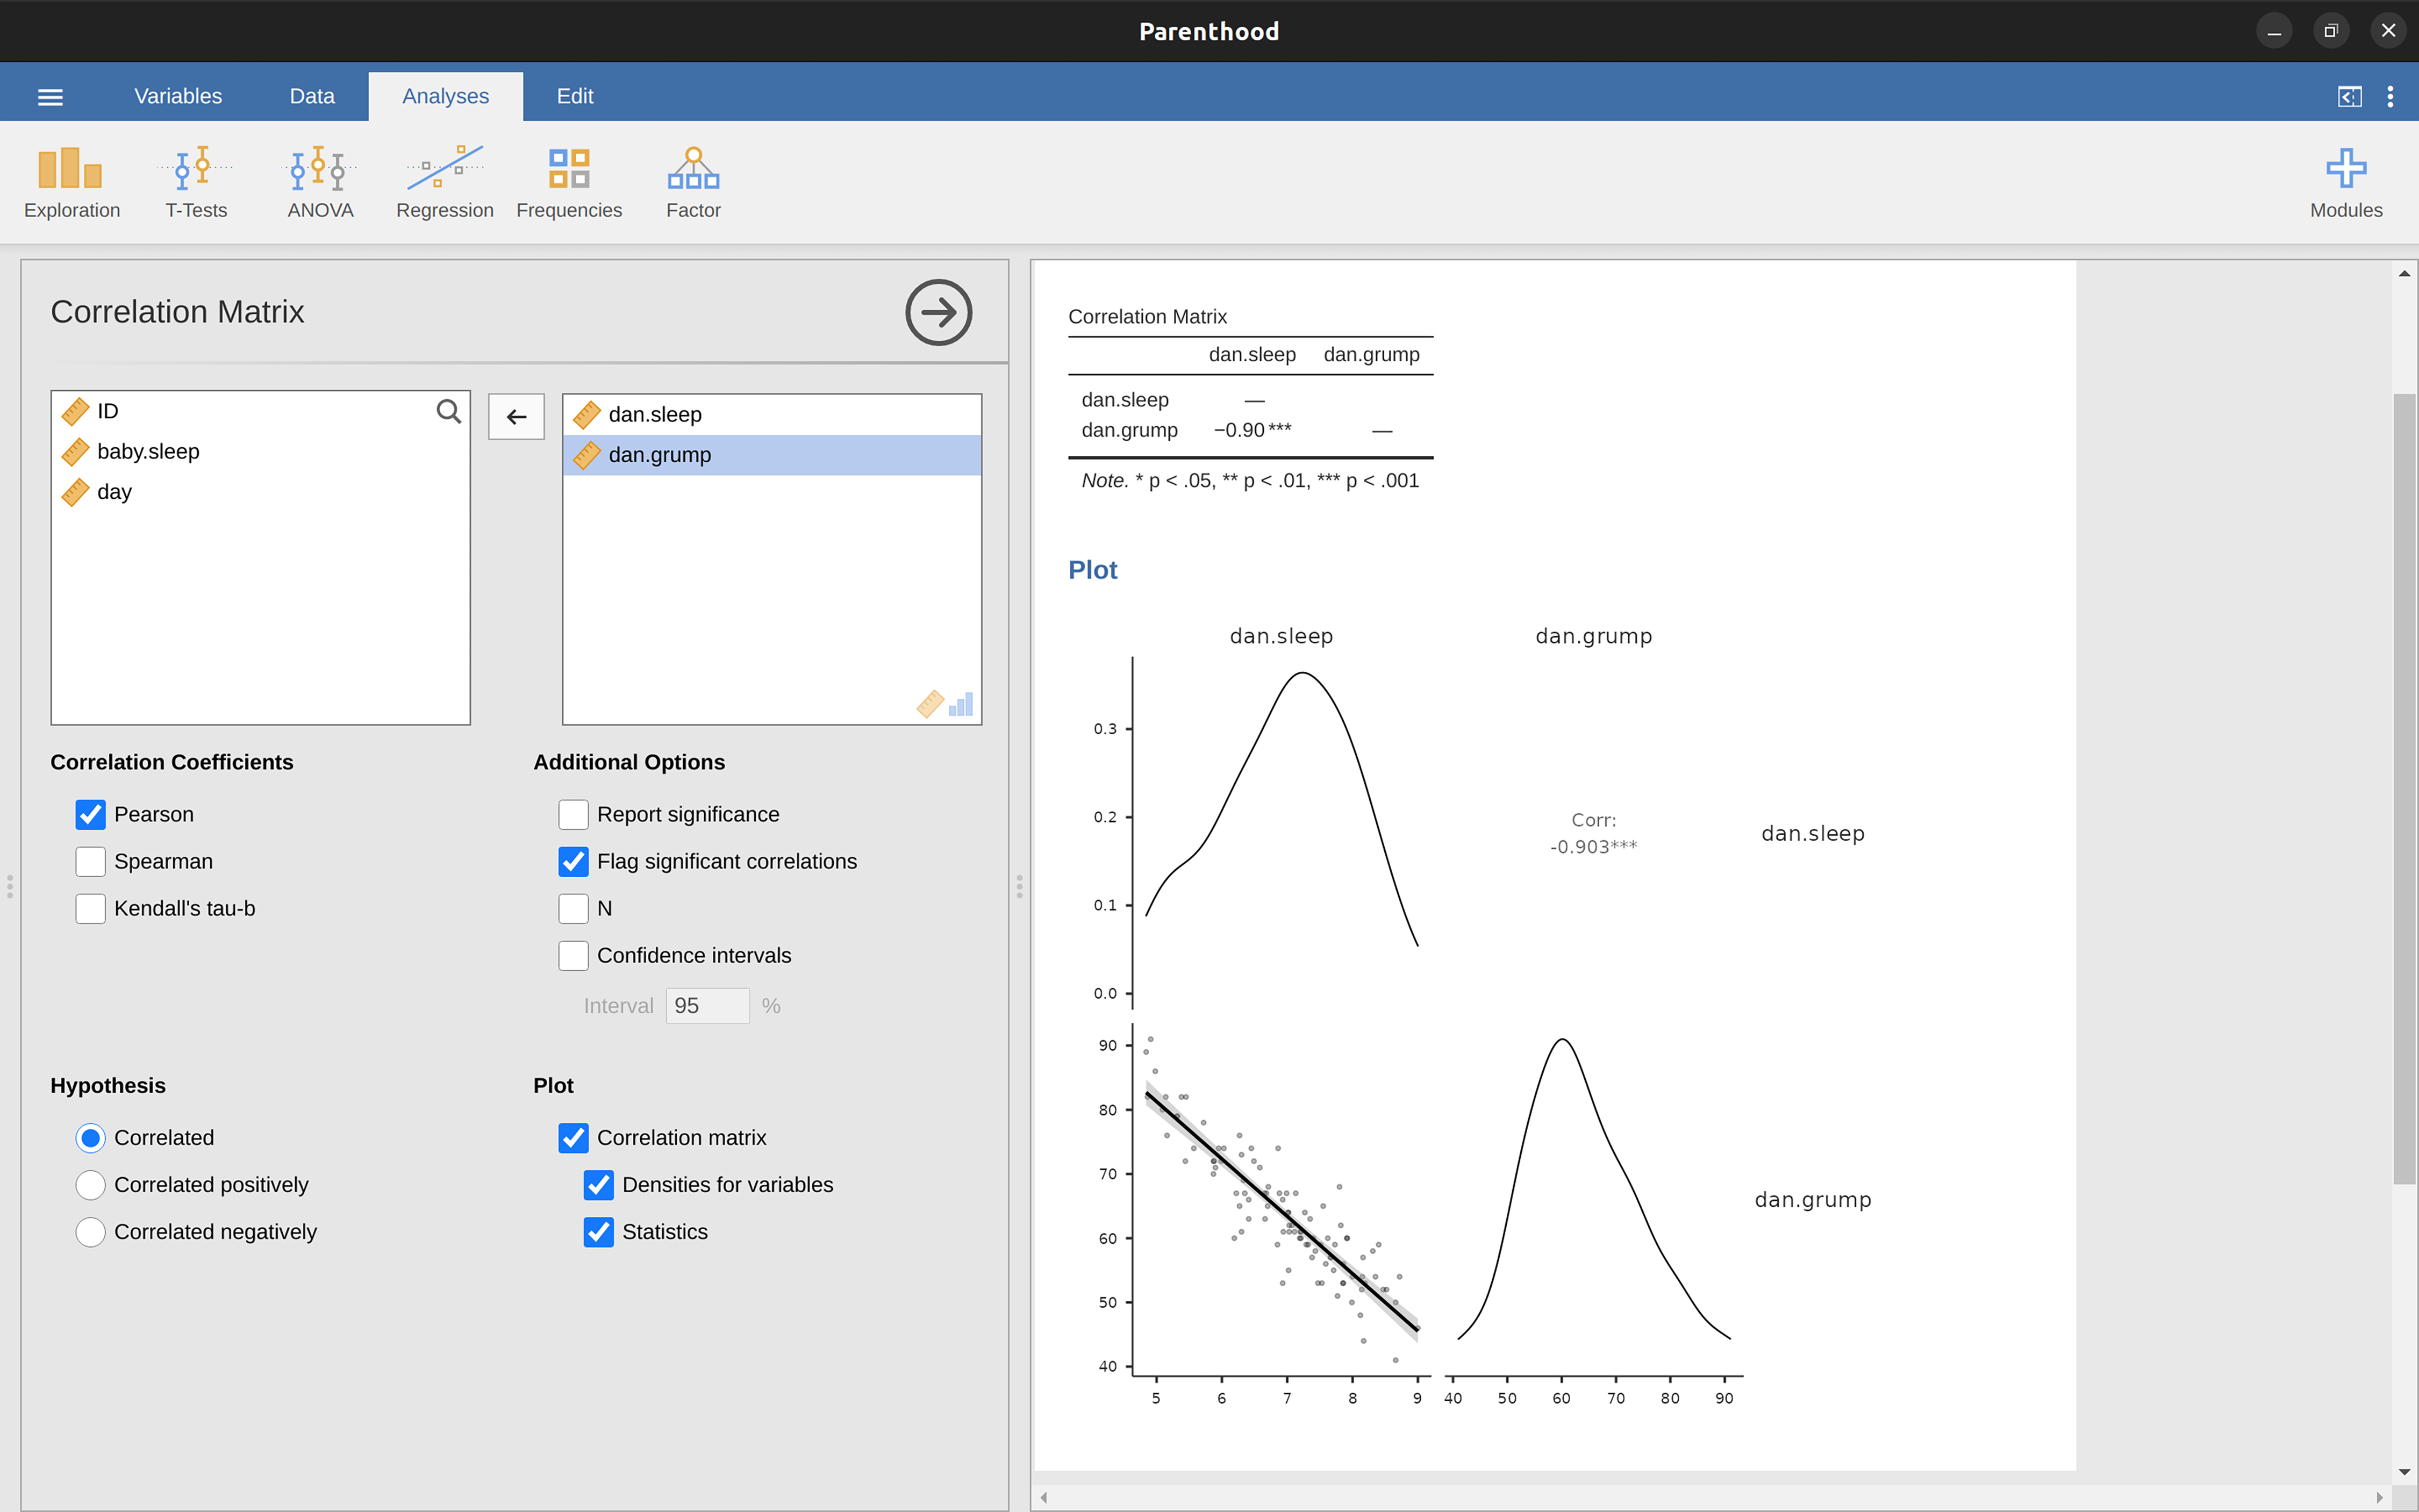
\includegraphics[width=1\textwidth,height=\textheight]{images/fig12-8.png} \hfill{}

\caption{\label{fig-fig12-8}Scatterplot via the `Correlation Matrix'
command in jamovi}

\end{figure}

The second way do to it is to use one of the jamovi add-on modules. This
module is called `scatr' and you can install it by clicking on the large
`\(+\)' icon in the top right of the jamovi screen, opening the jamovi
library, scrolling down until you find `scatr' and clicking `install'.
When you have done this, you will find a new `Scatterplot' command
available under the `Exploration' button. This plot is a bit different
than the first way, see Figure~\ref{fig-fig12-9}, but the important
information is the same.

\begin{figure}[h!]


\includegraphics[width=0.8\textwidth,height=\textheight]{images/fig12-9.png} \hfill{}

\caption{\label{fig-fig12-9}Scatterplot via the `scatr' add-on module in
jamovi}

\end{figure}

\hypertarget{more-elaborate-options}{%
\subsection{More elaborate options}\label{more-elaborate-options}}

Often you will want to look at the relationships between several
variables at once, using a \textbf{scatterplot matrix} (in jamovi via
the `Correlation Matrix' -- `Plot' command). Just add another variable,
for example baby.sleep to the list of variables to be correlated, and
jamovi will create a scatterplot matrix for you, just like the one in
Figure~\ref{fig-fig12-10}.

\hypertarget{what-is-a-linear-regression-model}{%
\section{What is a linear regression
model?}\label{what-is-a-linear-regression-model}}

Stripped to its bare essentials, linear regression models are basically
a slightly fancier version of the Pearson correlation (see
\protect\hyperlink{correlations}{Correlations}), but they are actually
much more powerful tools. We'll return to the \emph{parenthood.csv} file
that we were using to illustrate how correlations work. Recall that, in
this data set we were trying to find out why Dani is so very grumpy all
the time and our working hypothesis was that I'm not getting enough
sleep. We drew a scatterplots to help us examine the relationship
between the amount of sleep I get and my grumpiness the following day,
as in Figure~\ref{fig-fig12-9}, and as we saw that this corresponded to
a correlation of \(r = -.90\), but what we find ourselves secretly
imagining is something that looks closer to
Figure~\ref{fig-fig12-11}(a). That is, we mentally draw a straight line
through the middle of the data. In statistics, this line that we're
drawing is called a \textbf{regression line}. Notice that, since we're
not idiots, the regression line goes through the middle of the data. We
don't find ourselves imagining anything like the rather silly plot shown
in Figure~\ref{fig-fig12-11}(b).

\begin{figure}[h!]

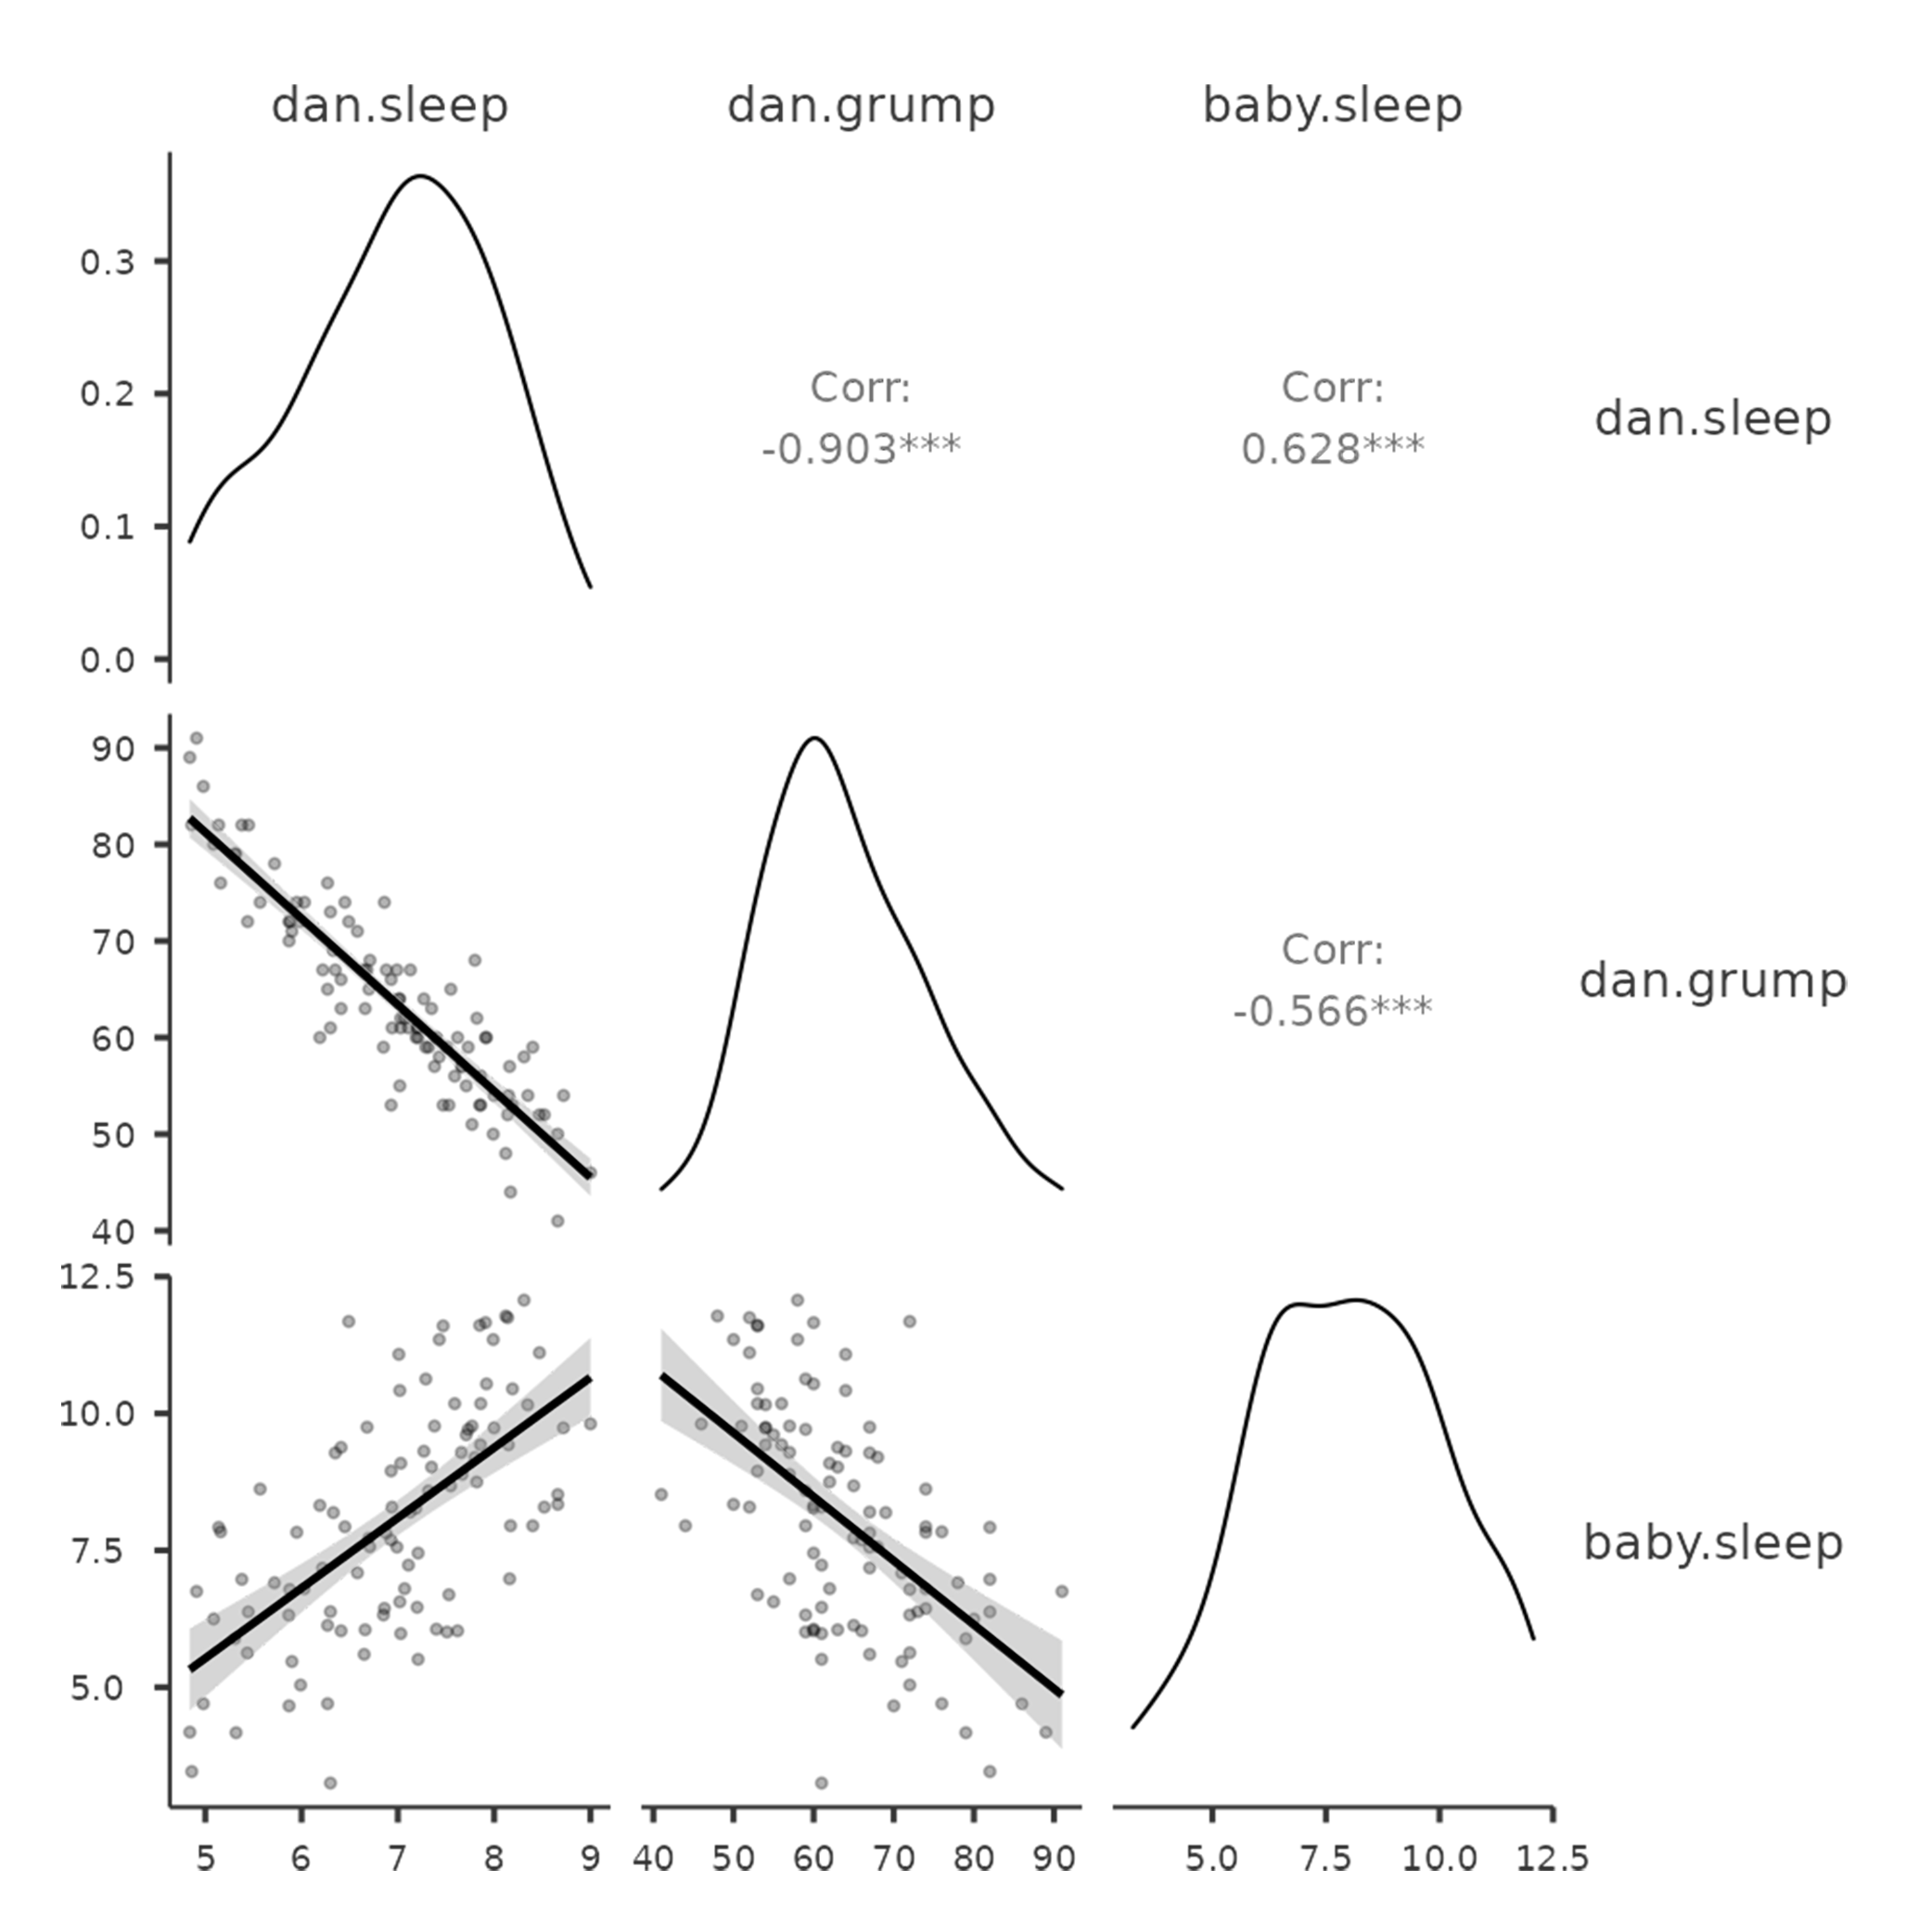
\includegraphics[width=1\textwidth,height=\textheight]{images/fig12-10.png} \hfill{}

\caption{\label{fig-fig12-10}A matrix of scatterplots produced using
jamovi}

\end{figure}

This is not highly surprising. The line that I've drawn in
Figure~\ref{fig-fig12-11}(b) doesn't ``fit'' the data very well, so it
doesn't make a lot of sense to propose it as a way of summarising the
data, right? This is a very simple observation to make, but it turns out
to be very powerful when we start trying to wrap just a little bit of
maths around it. To do so, let's start with a refresher of some high
school maths. The formula for a straight line is usually written like
this:

\[y=a+bx\]

\begin{figure}[H]

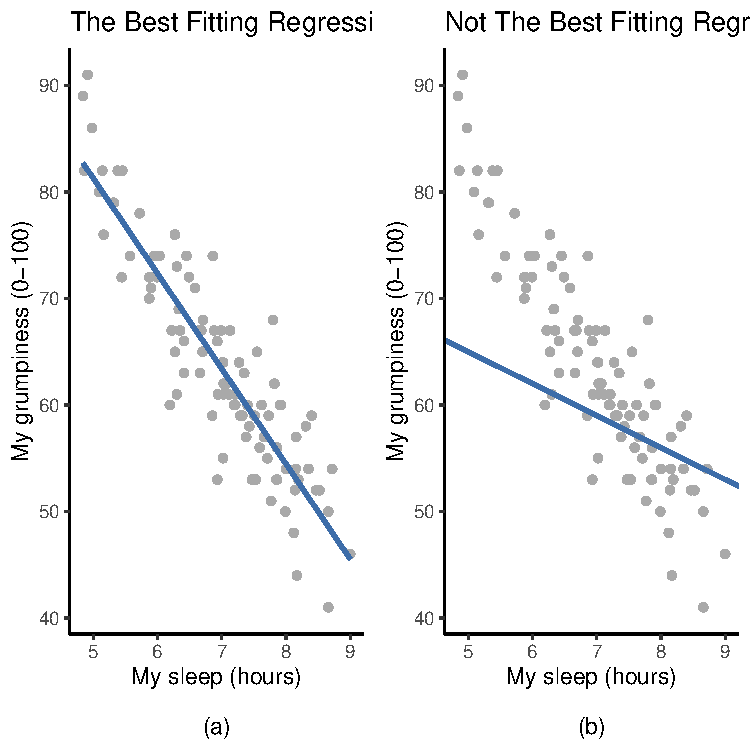
\includegraphics[width=1\textwidth,height=\textheight]{12-Correlation-and-linear-regression_files/figure-pdf/fig-fig12-11-1.pdf} \hfill{}

\caption{\label{fig-fig12-11}Panel (a) shows the sleep-grumpiness
scatterplot from Figure~\ref{fig-fig12-9} with the best fitting
regression line drawn over the top. Not surprisingly, the line goes
through the middle of the data. In contrast, panel (b) shows the same
data, but with a very poor choice of regression line drawn over the top}

\end{figure}

The two variables are \(x\) and \(y\), and we have two coefficients,
\(a\) and \(b\).\footnote{Also sometimes written as \(y = mx + c\) where
  \(m\) is the slope coefficient and \(c\) is the intercept (constant)
  coefficient: \[\hat{Y}_i=b_0+b_1X_i\]} The coefficient \(a\)
represents the y-intercept of the line, and coefficient \(b\) represents
the slope of the line. The intercept is interpreted as ``the value of y
that you get when \(x = 0\)''. Similarly, a slope of b means that if you
increase the x-value by 1 unit, then the y-value goes up by b units, and
a negative slope means that the y-value would go down rather than up. We
use the exact same formula for a regression line. If \(Y\) is the
outcome variable (the DV) and \(X\) is the predictor variable (the
\(IV\)), then the formula that describes our regression is written like
this:

\[\hat{Y}_i=b_0+b_1X_i\]

Hmm. Looks like the same formula, but there's some extra frilly bits in
this version. Let's make sure we understand them. Firstly, notice that
I've written \(X_i\) and \(Y_i\) rather than just plain old \(X\) and
\(Y\) . This is because we want to remember that we're dealing with
actual data. In this equation, \(X_i\) is the value of predictor
variable for the ith observation (i.e., the number of hours of sleep
that I got on day i of my little study), and \(Y_i\) is the
corresponding value of the outcome variable (i.e., my grumpiness on that
day). And although I haven't said so explicitly in the equation, what
we're assuming is that this formula works for all observations in the
data set (i.e., for all i). Secondly, notice that I wrote \(\hat{Y}_i\)
and not \(Y_i\) . This is because we want to make the distinction
between the actual data \(Y_i\), and the estimate \(\hat{Y}_i\) (i.e.,
the prediction that our regression line is making). Thirdly, I changed
the letters used to describe the coefficients from a and \(b\) to
\(b_0\) and \(b_1\). That's just the way that statisticians like to
refer to the coefficients in a regression model. I've no idea why they
chose b, but that's what they did. In any case \(b_0\) always refers to
the intercept term, and \(b_1\) refers to the slope.

Excellent, excellent. Next, I can't help but notice that, regardless of
whether we're talking about the good regression line or the bad one, the
data don't fall perfectly on the line. Or, to say it another way, the
data \(Y_i\) are not identical to the predictions of the regression
model \(\hat{Y}_i\). Since statisticians love to attach letters, names
and numbers to everything, let's refer to the difference between the
model prediction and that actual data point as a residual, and we'll
refer to it as \(\epsilon_i\).\footnote{The \(\epsilon\) symbol is the
  Greek letter epsilon. It's traditional to use \(\epsilon_i\) or
  \(e_i\) to denote a residual: \[\epsilon_i=Y_i-\hat{Y}_i\] which in
  turn means that we can write down the complete linear regression model
  as: \[Y_i=b_0+b_1X_i+\epsilon_i\]} Written using mathematics, the
residuals are defined as

\hypertarget{estimating-a-linear-regression-model}{%
\section{Estimating a linear regression
model}\label{estimating-a-linear-regression-model}}

Okay, now let's redraw our pictures but this time I'll add some lines to
show the size of the residual for all observations. When the regression
line is good, our residuals (the lengths of the solid black lines) all
look pretty small, as shown in Figure~\ref{fig-fig12-12}(a), but when
the regression line is a bad one the residuals are a lot larger, as you
can see from looking at Figure~\ref{fig-fig12-12}(b). Hmm. Maybe what we
``want'' in a regression model is \emph{small} residuals. Yes, that does
seem to make sense. In fact, I think I'll go so far as to say that the
``best fitting'' regression line is the one that has the smallest
residuals. Or, better yet, since statisticians seem to like to take
squares of everything why not say that:

\begin{quote}
The estimated regression coefficients, \(\hat{b}_0\) and \(\hat{b}_1\),
are those that minimise the sum of the squared residuals, which we could
either write as \(\sum_i (Y_i - \hat{Y}_i)^2\) or as
\(\sum_i \epsilon_i^2\).
\end{quote}

\begin{figure}[h!]

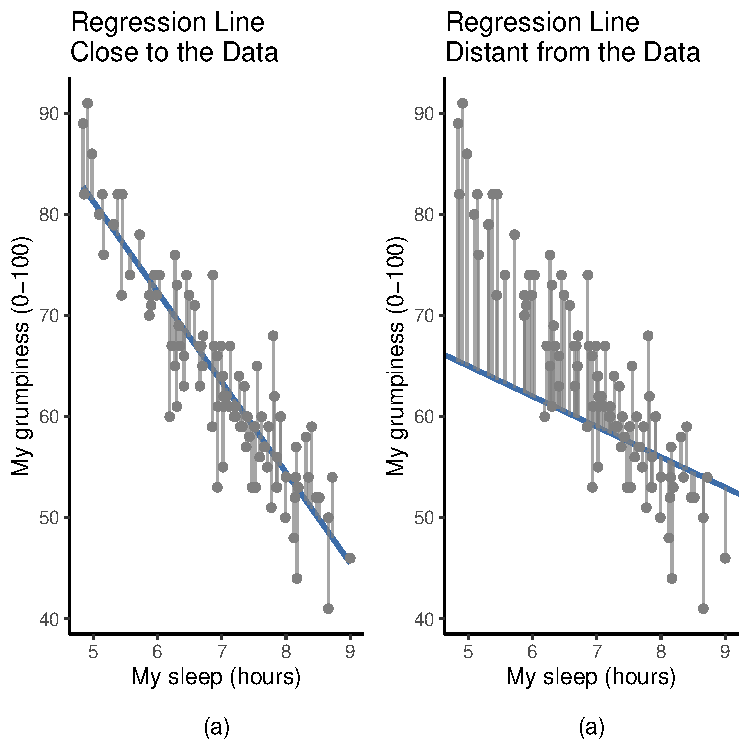
\includegraphics[width=1\textwidth,height=\textheight]{12-Correlation-and-linear-regression_files/figure-pdf/fig-fig12-12-1.pdf} \hfill{}

\caption{\label{fig-fig12-12}A depiction of the residuals associated
with the best fitting regression line (panel a), and the residuals
associated with a poor regression line (panel b). The residuals are much
smaller for the good regression line. Again, this is no surprise given
that the good line is the one that goes right through the middle of the
data}

\end{figure}

Yes, yes that sounds even better. And since I've indented it like that,
it probably means that this is the right answer. And since this is the
right answer, it's probably worth making a note of the fact that our
regression coefficients are estimates (we're trying to guess the
parameters that describe a population!), which is why I've added the
little hats, so that we get \(\hat{b}_0\) and \(\hat{b}_1\) rather than
\(b_0\) and \(b_1\). Finally, I should also note that, since there's
actually more than one way to estimate a regression model, the more
technical name for this estimation process is \textbf{ordinary least
squares (OLS) regression}.

At this point, we now have a concrete definition for what counts as our
``best'' choice of regression coefficients, \(\hat{b}_0\) and
\(\hat{b}_1\). The natural question to ask next is, if our optimal
regression coefficients are those that minimise the sum squared
residuals, how do we find these wonderful numbers? The actual answer to
this question is complicated and doesn't help you understand the logic
of regression.\footnote{Or at least, I'm assuming that it doesn't help
  most people. But on the off chance that someone reading this is a
  proper kung fu master of linear algebra (and to be fair, I always have
  a few of these people in my intro stats class), it will help you to
  know that the solution to the estimation problem turns out to be
  \(\hat{b} = (X^{'}X)^{-1}X^{'}y\), where \(\hat{b}\) is a vector
  containing the estimated regression coefficients, \(X\) is the
  ``design matrix'' that contains the predictor variables (plus an
  additional column containing all ones; strictly \(X\) is a matrix of
  the regressors, but I haven't discussed the distinction yet), and
  \(y\) is a vector containing the outcome variable. For everyone else,
  this isn't exactly helpful and can be downright scary. However, since
  quite a few things in linear regression can be written in linear
  algebra terms, you'll see a bunch of footnotes like this one in this
  chapter. If you can follow the maths in them, great. If not, ignore
  it.} This time I'm going to let you off the hook. Instead of showing
you the long and tedious way first and then ``revealing'' the wonderful
shortcut that jamovi provides, let's cut straight to the chase and just
use jamovi to do all the heavy lifting.

\hypertarget{linear-regression-in-jamovi}{%
\subsection{Linear regression in
jamovi}\label{linear-regression-in-jamovi}}

To run my linear regression, open up the `Regression' -- `Linear
Regression' analysis in jamovi, using the \emph{parenthood.csv} data
file. Then specify dani.grump as the `Dependent Variable' and dani.sleep
as the variable entered in the `Covariates' box. This gives the results
shown in Figure~\ref{fig-fig12-13}, showing an intercept
\(\hat{b}_0 = 125.96\) and the slope \(\hat{b}_1 = -8.94\). In other
words, the best fitting regression line that I plotted in
Figure~\ref{fig-fig12-12} has this formula:

\[\hat{Y}_i=125.96+(-8.94 X_i)\]

\begin{figure}[h!]

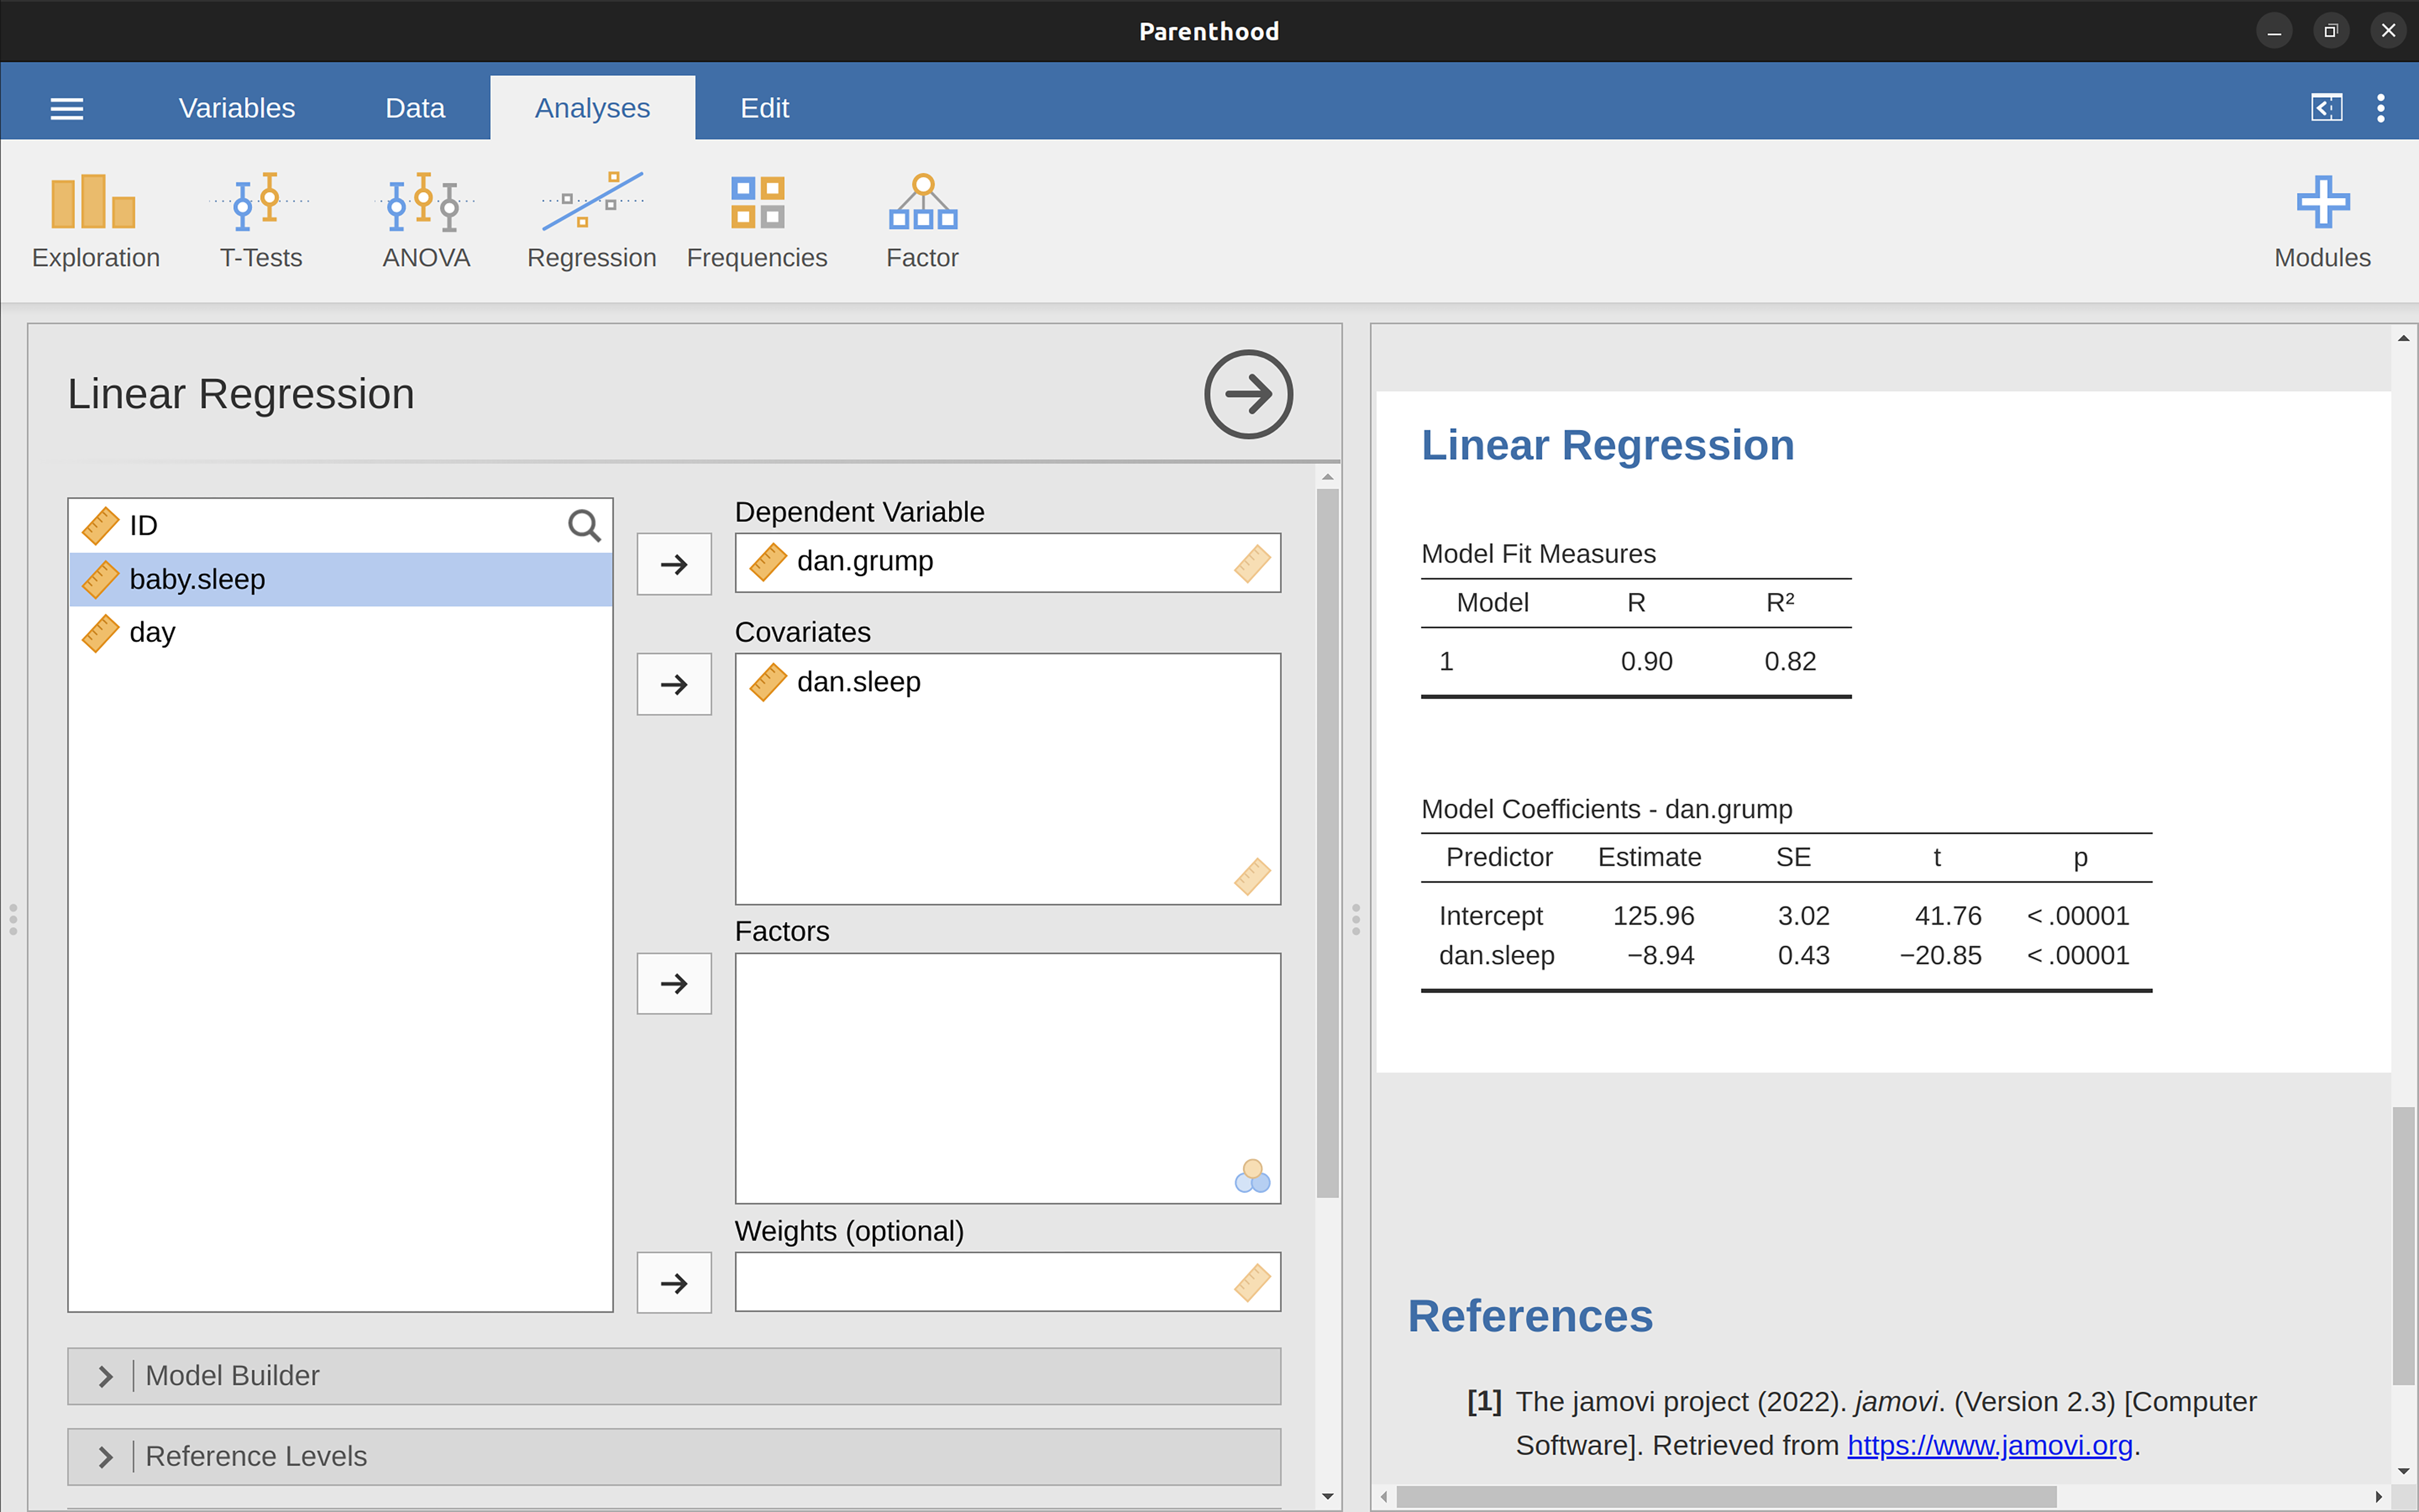
\includegraphics[width=1\textwidth,height=\textheight]{images/fig12-13.png} \hfill{}

\caption{\label{fig-fig12-13}A jamovi screenshot showing a simple linear
regression analysis}

\end{figure}

\hypertarget{interpreting-the-estimated-model}{%
\subsection{Interpreting the estimated
model}\label{interpreting-the-estimated-model}}

The most important thing to be able to understand is how to interpret
these coefficients. Let's start with \(\hat{b}_1\), the slope. If we
remember the definition of the slope, a regression coefficient of
\(\hat{b}_1 = -8.94\) means that if I increase \(X_i\) by 1, then I'm
decreasing \(Y_i\) by 8.94. That is, each additional hour of sleep that
I gain will improve my mood, reducing my grumpiness by 8.94 grumpiness
points. What about the intercept? Well, since \(\hat{b}_0\) corresponds
to ``the expected value of \(Y_i\) when \(X_i\) equals 0'', it's pretty
straightforward. It implies that if I get zero hours of sleep
(\(X_i = 0\)) then my grumpiness will go off the scale, to an insane
value of (\(Y_i = 125.96\)). Best to be avoided, I think.

\hypertarget{multiple-linear-regression}{%
\section{Multiple linear regression}\label{multiple-linear-regression}}

The simple linear regression model that we've discussed up to this point
assumes that there's a single predictor variable that you're interested
in, in this case dani.sleep. In fact, up to this point every statistical
tool that we've talked about has assumed that your analysis uses one
predictor variable and one outcome variable. However, in many (perhaps
most) research projects you actually have multiple predictors that you
want to examine. If so, it would be nice to be able to extend the linear
regression framework to be able to include multiple predictors. Perhaps
some kind of \textbf{multiple regression} model would be in order?

Multiple regression is conceptually very simple. All we do is add more
terms to our regression equation. Let's suppose that we've got two
variables that we're interested in; perhaps we want to use both
dani.sleep and baby.sleep to predict the dani.grump variable. As before,
we let \(Y_{i}\) refer to my grumpiness on the i-th day. But now we have
two \$ X \$ variables: the first corresponding to the amount of sleep I
got and the second corresponding to the amount of sleep my son got. So
we'll let \(X_{i1}\) refer to the hours I slept on the i-th day and
\(X_{i2}\) refers to the hours that the baby slept on that day. If so,
then we can write our regression model like this:
\[Y_i=b_0+b_1X_{i1}+b_2X_{i2}+\epsilon_i\]

As before, \(\epsilon_i\) is the residual associated with the i-th
observation, \(\epsilon_i = Y_i - \hat{Y}_i\). In this model, we now
have three coefficients that need to be estimated: \(b_0\) is the
intercept, \(b_1\) is the coefficient associated with my sleep, and
\(b_2\) is the coefficient associated with my son's sleep. However,
although the number of coefficients that need to be estimated has
changed, the basic idea of how the estimation works is unchanged: our
estimated coefficients \(\hat{b}_0\), \(\hat{b}_1\) and \(\hat{b}_2\)
are those that minimise the sum squared residuals.

\hypertarget{doing-it-in-jamovi}{%
\subsection{Doing it in jamovi}\label{doing-it-in-jamovi}}

Multiple regression in jamovi is no different to simple regression. All
we have to do is add additional variables to the `Covariates' box in
jamovi. For example, if we want to use both dani.sleep and baby.sleep as
predictors in our attempt to explain why I'm so grumpy, then move
baby.sleep across into the `Covariates' box alongside dani.sleep. By
default, jamovi assumes that the model should include an intercept. The
coefficients we get this time are shown in Table~\ref{tbl-tab12-4}.

\hypertarget{tbl-tab12-4}{}
 
  \providecommand{\huxb}[2]{\arrayrulecolor[RGB]{#1}\global\arrayrulewidth=#2pt}
  \providecommand{\huxvb}[2]{\color[RGB]{#1}\vrule width #2pt}
  \providecommand{\huxtpad}[1]{\rule{0pt}{#1}}
  \providecommand{\huxbpad}[1]{\rule[-#1]{0pt}{#1}}

\begin{table}[ht]
\caption{\label{tbl-tab12-4}Adding multiple variables as predictors in a regression }\tabularnewline

\begin{centerbox}
\begin{threeparttable}
\setlength{\tabcolsep}{0pt}
\begin{tabularx}{0.9\textwidth}{p{0.3\textwidth} p{0.3\textwidth} p{0.3\textwidth}}


\hhline{>{\huxb{0, 0, 0}{0.4}}->{\huxb{0, 0, 0}{0.4}}->{\huxb{0, 0, 0}{0.4}}-}
\arrayrulecolor{black}

\multicolumn{1}{!{\huxvb{0, 0, 0}{0}}p{0.3\textwidth}!{\huxvb{0, 0, 0}{0}}}{\hspace{0pt}\parbox[b]{0.3\textwidth-0pt-12pt}{\huxtpad{2pt + 1em}\centering \textbf{(Intercept)}\huxbpad{2pt}}} &
\multicolumn{1}{p{0.3\textwidth}!{\huxvb{0, 0, 0}{0}}}{\hspace{12pt}\parbox[b]{0.3\textwidth-12pt-12pt}{\huxtpad{2pt + 1em}\centering \textbf{dani.sleep}\huxbpad{2pt}}} &
\multicolumn{1}{p{0.3\textwidth}!{\huxvb{0, 0, 0}{0}}}{\hspace{12pt}\parbox[b]{0.3\textwidth-12pt-0pt}{\huxtpad{2pt + 1em}\centering \textbf{baby.sleep}\huxbpad{2pt}}} \tabularnewline[-0.5pt]


\hhline{>{\huxb{0, 0, 0}{0.4}}->{\huxb{0, 0, 0}{0.4}}->{\huxb{0, 0, 0}{0.4}}-}
\arrayrulecolor{black}

\multicolumn{1}{!{\huxvb{0, 0, 0}{0}}p{0.3\textwidth}!{\huxvb{0, 0, 0}{0}}}{\hspace{0pt}\parbox[b]{0.3\textwidth-0pt-12pt}{\huxtpad{2pt + 1em}\centering 125.97\huxbpad{2pt}}} &
\multicolumn{1}{p{0.3\textwidth}!{\huxvb{0, 0, 0}{0}}}{\hspace{12pt}\parbox[b]{0.3\textwidth-12pt-12pt}{\huxtpad{2pt + 1em}\centering -8.95\huxbpad{2pt}}} &
\multicolumn{1}{p{0.3\textwidth}!{\huxvb{0, 0, 0}{0}}}{\hspace{12pt}\parbox[b]{0.3\textwidth-12pt-0pt}{\huxtpad{2pt + 1em}\centering 0.01\huxbpad{2pt}}} \tabularnewline[-0.5pt]


\hhline{>{\huxb{0, 0, 0}{0.4}}->{\huxb{0, 0, 0}{0.4}}->{\huxb{0, 0, 0}{0.4}}-}
\arrayrulecolor{black}
\end{tabularx} 

\end{threeparttable}\par\end{centerbox}

\end{table}
 

The coefficient associated with dani.sleep is quite large, suggesting
that every hour of sleep I lose makes me a lot grumpier. However, the
coefficient for baby.sleep is very small, suggesting that it doesn't
really matter how much sleep my son gets. What matters as far as my
grumpiness goes is how much sleep I get. To get a sense of what this
multiple regression model looks like, Figure~\ref{fig-fig12-14} shows a
3D plot that plots all three variables, along with the regression model
itself.

{[}Additional technical detail\footnote{The formula for the general
  case: The equation that I gave in the main text shows you what a
  multiple regression model looks like when you include two predictors.
  Not surprisingly then, if you want more than two predictors all you
  have to do is add more \(X\) terms and more \(b\) coefficients. In
  other words, if you have \(K\) predictor variables in the model then
  the regression equation look like this:
  \[Y_i=b_0+(\sum_{k=1}^{K}b_k X_{ik})+\epsilon_i\]}{]}

\begin{figure}[h!]

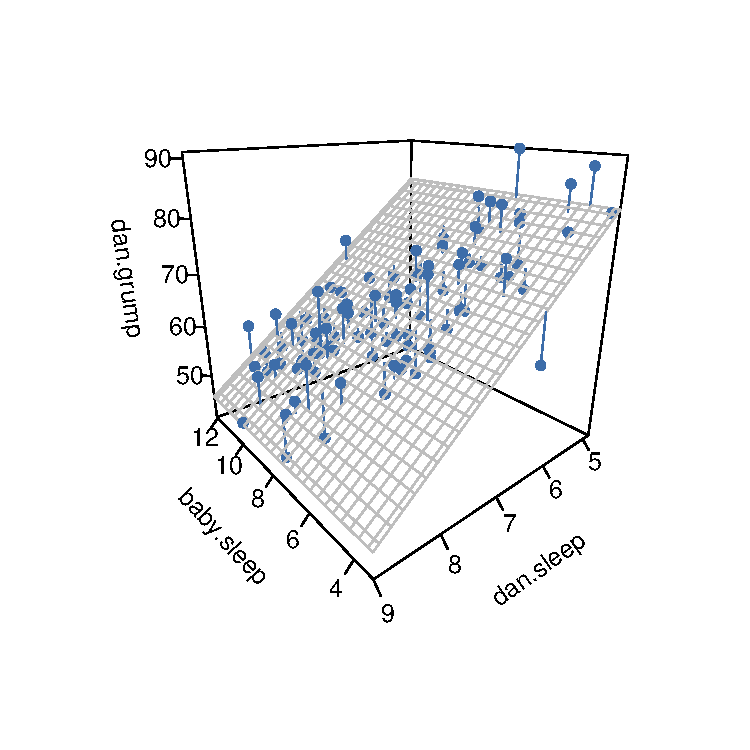
\includegraphics[width=1\textwidth,height=\textheight]{12-Correlation-and-linear-regression_files/figure-pdf/fig-fig12-14-1.pdf} \hfill{}

\caption{\label{fig-fig12-14}A 3D visualisation of a multiple regression
model. There are two predictors in the model, dani.sleep and baby.sleep
and the outcome variable is dani.grump. Together, these three variables
form a 3D space. Each observation (dot) is a point in this space. In
much the same way that a simple linear regression model forms a line in
2D space, this multiple regression model forms a plane in 3D space. When
we estimate the regression coefficients what we're trying to do is find
a plane that is as close to all the blue dots as possible}

\end{figure}

\hypertarget{quantifying-the-fit-of-the-regression-model}{%
\section{Quantifying the fit of the regression
model}\label{quantifying-the-fit-of-the-regression-model}}

So we now know how to estimate the coefficients of a linear regression
model. The problem is, we don't yet know if this regression model is any
good. For example, the regression.1 model claims that every hour of
sleep will improve my mood by quite a lot, but it might just be rubbish.
Remember, the regression model only produces a prediction \(\hat{Y}_i\)
about what my mood is like, but my actual mood is \(Y_i\) . If these two
are very close, then the regression model has done a good job. If they
are very different, then it has done a bad job.

\hypertarget{sec-The-R2-value}{%
\subsection{\texorpdfstring{The \(R^2\)
value}{The R\^{}2 value}}\label{sec-The-R2-value}}

Once again, let's wrap a little bit of mathematics around this. Firstly,
we've got the sum of the squared residuals:

\[SS_{res}=\sum_i (Y_i-\hat{Y_i})^2\]

which we would hope to be pretty small. Specifically, what we'd like is
for it to be very small in comparison to the total variability in the
outcome variable:

\[SS_{tot}=\sum_i(Y_i-\bar{Y})^2\]

While we're here, let's calculate these values ourselves, not by hand
though. Let's use something like Excel or another standard spreadsheet
programme. I have done this by opening up the \emph{parenthood.csv} file
in Excel and saving it as parenthood rsquared.xls so that I can work on
it. The first thing to do is calculate the \(\hat{Y}\) values, and for
the simple model that uses only a single predictor we would do the
following:

\begin{enumerate}
\def\labelenumi{\arabic{enumi}.}
\tightlist
\item
  Create a new column called ' Y.pred ' using the formula ' = 125.97 +
  (-8.94 \(\times\) dani.sleep) '.
\item
  Calculate the \(SS_{resid}\) by creating a new column called '
  (Y-Y.pred)\^{}2 ' using the formula ' = (dani.grump - Y.pred)\^{}2 '.
\item
  Then, at the bottom of this column calculate the sum of these values,
  i.e.~' sum( ( Y-Y.pred)\^{}2 ) '.
\item
  At the bottom of the dani.grump column, calculate the mean value for
  dani.grump (NB Excel uses the word ' AVERAGE ' rather than ' mean ' in
  its function).
\item
  Then create a new column, called ' (Y - mean(Y))\^{}2 ) ' using the
  formula ' = (dani.grump - AVERAGE(dani.grump))\^{}2 '.
\item
  Then, at the bottom of this column calculate the sum of these values,
  i.e.~`sum( (Y - mean(Y))\^{}2 )'.
\item
  Calculate \(R^2\) by typing into a blank cell the following: `= 1 -
  (SS(resid) / SS(tot) )'.
\end{enumerate}

This gives a value for \(R^2\) of `0.8161018'. The \(R^2\) value,
sometimes called the \textbf{coefficient of determination}\footnote{And
  by ``sometimes'' I mean ``almost never''. In practice everyone just
  calls it ``R-squared''.} has a simple interpretation: it is the
proportion of the variance in the outcome variable that can be accounted
for by the predictor. So, in this case the fact that we have obtained
\(R^2 = .816\) means that the predictor (my.sleep) explains \(81.6\%\)
of the variance in the outcome (my.grump).

Naturally, you don't actually need to type all these commands into Excel
yourself if you want to obtain the \(R^2\) value for your regression
model. As we'll see later on in the section on
\protect\hyperlink{running-the-hypothesis-tests-in-jamovi}{Running the
hypothesis tests in jamovi}, all you need to do is specify this as an
option in jamovi. However, let's put that to one side for the moment.
There's another property of \(R^2\) that I want to point out.

\hypertarget{the-relationship-between-regression-and-correlation}{%
\subsection{The relationship between regression and
correlation}\label{the-relationship-between-regression-and-correlation}}

At this point we can revisit my earlier claim that regression, in this
very simple form that I've discussed so far, is basically the same thing
as a correlation. Previously, we used the symbol \(r\) to denote a
Pearson correlation. Might there be some relationship between the value
of the correlation coefficient \(r\) and the \(R^2\) value from linear
regression? Of course there is: the squared correlation \(r^2\) is
identical to the \(R^2\) value for a linear regression with only a
single predictor. In other words, running a Pearson correlation is more
or less equivalent to running a linear regression model that uses only
one predictor variable.

\hypertarget{the-adjusted-r2-value}{%
\subsection{\texorpdfstring{The adjusted \(R^2\)
value}{The adjusted R\^{}2 value}}\label{the-adjusted-r2-value}}

One final thing to point out before moving on. It's quite common for
people to report a slightly different measure of model performance,
known as ``adjusted \(R^2\)''. The motivation behind calculating the
adjusted \(R^2\) value is the observation that adding more predictors
into the model will always cause the \(R^2\) value to increase (or at
least not decrease).

{[}Additional technical detail\footnote{The adjusted \(R^2\) value
  introduces a slight change to the calculation, as follows. For a
  regression model with \(K\) predictors, fit to a data set containing
  \(N\) observations, the adjusted \(R^2\) is:
  \[\text{adj.}R^2=1-(\frac{SS_{res}}{SS_{tot}} \times \frac{N-1}{N-K-1})\]}{]}

This adjustment is an attempt to take the degrees of freedom into
account. The big advantage of the adjusted \(R^2\) value is that when
you add more predictors to the model, the adjusted \(R^2\) value will
only increase if the new variables improve the model performance more
than you'd expect by chance. The big disadvantage is that the adjusted
\(R^2\) value can't be interpreted in the elegant way that \(R^2\) can.
\(R^2\) has a simple interpretation as the proportion of variance in the
outcome variable that is explained by the regression model. To my
knowledge, no equivalent interpretation exists for adjusted \(R^2\).

An obvious question then is whether you should report \(R^2\) or
adjusted \(R^2\). This is probably a matter of personal preference. If
you care more about interpretability, then \(R^2\) is better. If you
care more about correcting for bias, then adjusted \(R^2\) is probably
better. Speaking just for myself, I prefer \(R^2\). My feeling is that
it's more important to be able to interpret your measure of model
performance. Besides, as we'll see in
\protect\hyperlink{hypothesis-tests-for-regression-models}{Hypothesis
tests for regression models}, if you're worried that the improvement in
\(R^2\) that you get by adding a predictor is just due to chance and not
because it's a better model, well we've got hypothesis tests for that.

\hypertarget{hypothesis-tests-for-regression-models}{%
\section{Hypothesis tests for regression
models}\label{hypothesis-tests-for-regression-models}}

So far we've talked about what a regression model is, how the
coefficients of a regression model are estimated, and how we quantify
the performance of the model (the last of these, incidentally, is
basically our measure of effect size). The next thing we need to talk
about is hypothesis tests. There are two different (but related) kinds
of hypothesis tests that we need to talk about: those in which we test
whether the regression model as a whole is performing significantly
better than a null model, and those in which we test whether a
particular regression coefficient is significantly different from zero.

\hypertarget{testing-the-model-as-a-whole}{%
\subsection{Testing the model as a
whole}\label{testing-the-model-as-a-whole}}

Okay, suppose you've estimated your regression model. The first
hypothesis test you might try is the null hypothesis that there is no
relationship between the predictors and the outcome, and the alternative
hypothesis that the data are distributed in exactly the way that the
regression model predicts.

{[}Additional technical detail\footnote{Formally, our ``null model''
  corresponds to the fairly trivial ``regression'' model in which we
  include 0 predictors and only include the intercept term \(b_0\):
  \(H_0:Y_0=b_0+\epsilon_i\) If our regression model has \(K\)
  predictors, the ``alternative model'' is described using the usual
  formula for a multiple regression model:
  \[H_1:Y_i=b_0+(\sum_{k=1}^K b_k X_{ik})+\epsilon_i\] How can we test
  these two hypotheses against each other? The trick is to understand
  that it's possible to divide up the total variance \(SStot\) into the
  sum of the residual variance \(SSres\) and the regression model
  variance \(SSmod\). I'll skip over the technicalities, since we'll get
  to that later when we look at ANOVA in
  \textbf{?@sec-Comparing-several-means-one-way-ANOVA}. But just note
  that \(SS_{mod}=SS_{tot}-SS_{res}\) And we can convert the sums of
  squares into mean squares by dividing by the degrees of freedom:
  \[MS_{mod}=\frac{SS_{mod}}{df_{mod}}\]
  \[MS_{res}=\frac{SS_{res}}{df_{res}}\] So, how many degrees of freedom
  do we have? As you might expect the df associated with the model is
  closely tied to the number of predictors that we've included. In fact,
  it turns out that \(df_mod = K\). For the residuals the total degrees
  of freedom is \(df_res = N - K - 1\). Now that we've got our mean
  square values we can calculate an \(F\)-statistic like this:
  \[F=\frac{MS_{mod}}{MS_{res}}\] and the degrees of freedom associated
  with this are \(K\) and \(N - K - 1\).}{]}

We'll see much more of the \(F\)-statistic in
\textbf{?@sec-Comparing-several-means-one-way-ANOVA}, but for now just
know that we can interpret large \(F\)-values as indicating that the
null hypothesis is performing poorly in comparison to the alternative
hypothesis. In a moment I'll show you how to do the test in jamovi the
easy way, but first let's have a look at the tests for the individual
regression coefficients.

\hypertarget{tests-for-individual-coefficients}{%
\subsection{Tests for individual
coefficients}\label{tests-for-individual-coefficients}}

The \(F\)-test that we've just introduced is useful for checking that
the model as a whole is performing better than chance. If your
regression model doesn't produce a significant result for the \(F\)-test
then you probably don't have a very good regression model (or, quite
possibly, you don't have very good data). However, while failing this
test is a pretty strong indicator that the model has problems, passing
the test (i.e., rejecting the null) doesn't imply that the model is
good! Why is that, you might be wondering? The answer to that can be
found by looking at the coefficients for the
\protect\hyperlink{multiple-linear-regression}{Multiple linear
regression} model we have already looked at (Table~\ref{tbl-tab12-4})

I can't help but notice that the estimated regression coefficient for
the baby.sleep variable is tiny (\(0.01\)), relative to the value that
we get for dani.sleep (\(-8.95\)). Given that these two variables are
absolutely on the same scale (they're both measured in ``hours slept''),
I find this illuminating. In fact, I'm beginning to suspect that it's
really only the amount of sleep that I get that matters in order to
predict my grumpiness. We can re-use a hypothesis test that we discussed
earlier, the \(t\)-test. The test that we're interested in has a null
hypothesis that the true regression coefficient is zero (\(b = 0\)),
which is to be tested against the alternative hypothesis that it isn't
(\(b \neq 0\)). That is:

\[H_0:b=0\] \[H_1:b \neq 0\]

How can we test this? Well, if the central limit theorem is kind to us
we might be able to guess that the sampling distribution of \(\hat{b}\),
the estimated regression coefficient, is a normal distribution with mean
centred on \(b\). What that would mean is that if the null hypothesis
were true, then the sampling distribution of \(\hat{b}\) has mean zero
and unknown standard deviation. Assuming that we can come up with a good
estimate for the standard error of the regression coefficient,
\(se(\hat{b})\), then we're in luck. That's exactly the situation for
which we introduced the one-sample \(t\)-test back in
\textbf{?@sec-Comparing-two-means}. So let's define a \(t\)-statistic
like this:

\[t=\frac{\hat{b}}{SE(\hat{b})}\]

I'll skip over the reasons why, but our degrees of freedom in this case
are \(df = N - K - 1\). Irritatingly, the estimate of the standard error
of the regression coefficient, \(se(\hat{b})\), is not as easy to
calculate as the standard error of the mean that we used for the simpler
\(t\)-tests in \textbf{?@sec-Comparing-two-means}. In fact, the formula
is somewhat ugly, and not terribly helpful to look at.\footnote{For
  advanced readers only. The vector of residuals is
  \(\epsilon=y - X\hat{b}\). For K predictors plus the intercept, the
  estimated residual variance is
  \(\hat{\sigma}^2 = \frac{\epsilon^{'}\epsilon}{(N - K - 1)}\). The
  estimated covariance matrix of the coefficients is
  \(\hat{\sigma}^{2}(X^{'}X)^{-1}\), the main diagonal of which is
  \(se(\hat{b})\), our estimated standard errors.} For our purposes it's
sufficient to point out that the standard error of the estimated
regression coefficient depends on both the predictor and outcome
variables, and it is somewhat sensitive to violations of the homogeneity
of variance assumption (discussed shortly).

In any case, this \(t\)-statistic can be interpreted in the same way as
the \(t\)-statistics that we discussed in
\textbf{?@sec-Comparing-two-means}. Assuming that you have a two-sided
alternative (i.e., you don't really care if b \(>\) 0 or b \(<\) 0),
then it's the extreme values of t (i.e., a lot less than zero or a lot
greater than zero) that suggest that you should reject the null
hypothesis.

\hypertarget{running-the-hypothesis-tests-in-jamovi}{%
\subsection{Running the hypothesis tests in
jamovi}\label{running-the-hypothesis-tests-in-jamovi}}

To compute all of the statistics that we have talked about so far, all
you need to do is make sure the relevant options are checked in jamovi
and then run the regression. If we do that, as in
Figure~\ref{fig-fig12-15}, we get a whole bunch of useful output.

The `Model Coefficients' at the bottom of the jamovi analysis results
shown in Figure~\ref{fig-fig12-15} provides the coefficients of the
regression model. Each row in this table refers to one of the
coefficients in the regression model. The first row is the intercept
term, and the later ones look at each of the predictors. The columns
give you all of the relevant information. The first column is the actual
estimate of \(b\) (e.g., \(125.97\) for the intercept, and -8.95 for the
dani.sleep predictor). The second column is the standard error estimate
\(\hat{\sigma}_b\). The third and fourth columns provide the lower and
upper values for the 95\% confidence interval around the \(b\) estimate
(more on this later). The fifth column gives you the \(t\)-statistic,
and it's worth noticing that in this table
\(t=\frac{\hat{b}} {se({\hat{b}})}\) every time. Finally, the last
column gives you the actual \(p\)-value for each of these
tests.\footnote{Note that, although jamovi has done multiple tests here,
  it hasn't done a Bonferroni correction or anything (see
  \textbf{?@sec-Comparing-several-means-one-way-ANOVA}). These are
  standard one-sample \(t\)-tests with a two-sided alternative. If you
  want to make corrections for multiple tests, you need to do that
  yourself.}

\begin{figure}[H]

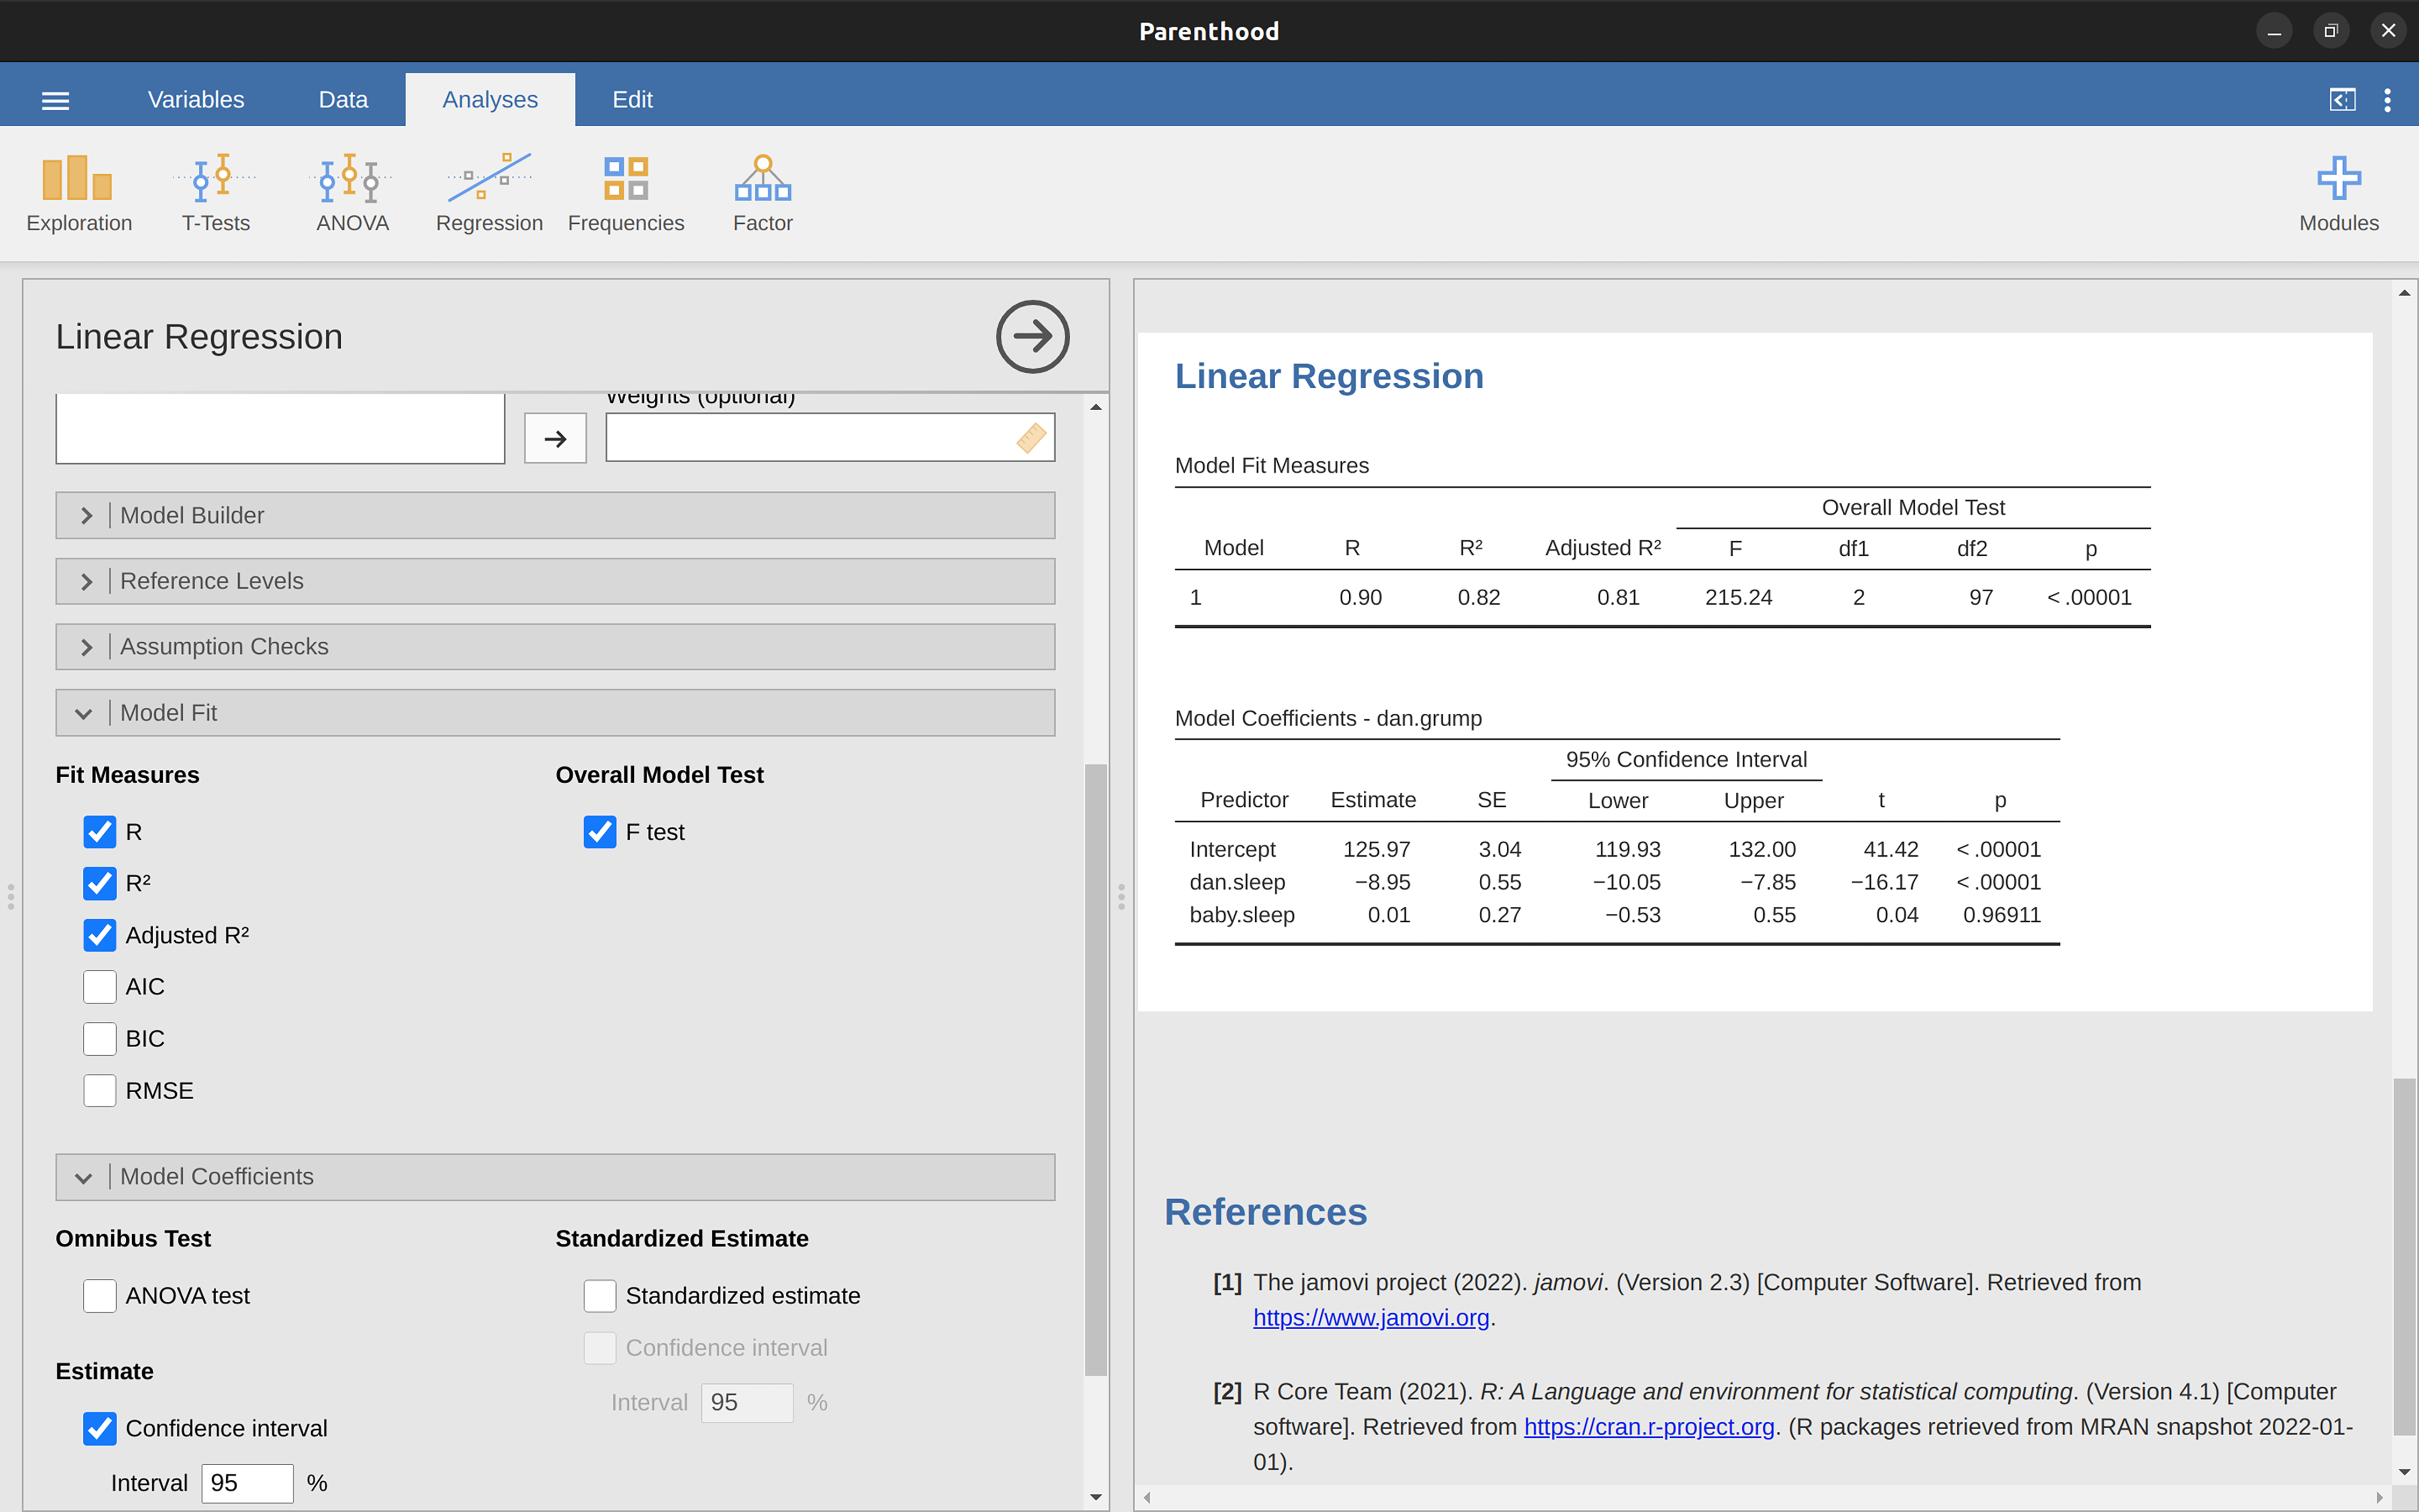
\includegraphics[width=1\textwidth,height=\textheight]{images/fig12-15.png} \hfill{}

\caption{\label{fig-fig12-15}A jamovi screenshot showing a multiple
linear regression analysis, with some useful options checked}

\end{figure}

The only thing that the coefficients table itself doesn't list is the
degrees of freedom used in the \(t\)-test, which is always \(N - K - 1\)
and is listed in the table at the top of the output, labelled `Model Fit
Measures'. We can see from this table that the model performs
significantly better than you'd expect by chance
(\(F(2,97) = 215.24, p< .001\)), which isn't all that surprising: the
\(R^2 = .81\) value indicate that the regression model accounts for
\(81\%\) of the variability in the outcome measure (and \(82\%\) for the
adjusted \(R^2\) ). However, when we look back up at the \(t\)-tests for
each of the individual coefficients, we have pretty strong evidence that
the baby.sleep variable has no significant effect. All the work in this
model is being done by the dani.sleep variable. Taken together, these
results suggest that this regression model is actually the wrong model
for the data. You'd probably be better off dropping the baby.sleep
predictor entirely. In other words, the simple regression model that we
started with is the better model.

\hypertarget{regarding-regression-coefficients}{%
\section{Regarding regression
coefficients}\label{regarding-regression-coefficients}}

Before moving on to discuss the assumptions underlying linear regression
and what you can do to check if they're being met, there's two more
topics I want to briefly discuss, both of which relate to the regression
coefficients. The first thing to talk about is calculating confidence
intervals for the coefficients. After that, I'll discuss the somewhat
murky question of how to determine which predictor is most important.

\hypertarget{confidence-intervals-for-the-coefficients}{%
\subsection{Confidence intervals for the
coefficients}\label{confidence-intervals-for-the-coefficients}}

Like any population parameter, the regression coefficients \(b\) cannot
be estimated with complete precision from a sample of data; that's part
of why we need hypothesis tests. Given this, it's quite useful to be
able to report confidence intervals that capture our uncertainty about
the true value of \(b\). This is especially useful when the research
question focuses heavily on an attempt to find out how strongly variable
\(X\) is related to variable \(Y\), since in those situations the
interest is primarily in the regression weight \(b\).

{[}Additional technical detail\footnote{Fortunately, confidence
  intervals for the regression weights can be constructed in the usual
  fashion \(CI(b)=\hat{b} \pm (t_{crit} \times SE(\hat{b}))\) where
  \(se(\hat{b})\) is the standard error of the regression coefficient,
  and \(t_crit\) is the relevant critical value of the appropriate
  \(t\)-distribution. For instance, if it's a 95\% confidence interval
  that we want, then the critical value is the \(97.5\)th quantile of a
  \(t\)-distribution with \(N -K -1\) degrees of freedom. In other
  words, this is basically the same approach to calculating confidence
  intervals that we've used throughout.}{]}

In jamovi we had already specified the `95\% Confidence interval' as
shown in Figure~\ref{fig-fig12-15}, although we could easily have chosen
another value, say a `99\% Confidence interval' if that is what we
decided on.

\hypertarget{calculating-standardised-regression-coefficients}{%
\subsection{Calculating standardised regression
coefficients}\label{calculating-standardised-regression-coefficients}}

One more thing that you might want to do is to calculate
``standardised'' regression coefficients, often denoted \(\beta\). The
rationale behind standardised coefficients goes like this. In a lot of
situations, your variables are on fundamentally different scales.
Suppose, for example, my regression model aims to predict people's
\(IQ\) scores using their educational attainment (number of years of
education) and their income as predictors. Obviously, educational
attainment and income are not on the same scales. The number of years of
schooling might only vary by 10s of years, whereas income can vary by
10,000s of dollars (or more). The units of measurement have a big
influence on the regression coefficients. The \(b\) coefficients only
make sense when interpreted in light of the units, both of the predictor
variables and the outcome variable. This makes it very difficult to
compare the coefficients of different predictors. Yet there are
situations where you really do want to make comparisons between
different coefficients. Specifically, you might want some kind of
standard measure of which predictors have the strongest relationship to
the outcome. This is what \textbf{standardised coefficients} aim to do.

The basic idea is quite simple; the standardised coefficients are the
coefficients that you would have obtained if you'd converted all the
variables to \emph{z}-scores before running the regression.\footnote{Strictly,
  you standardise all the \emph{regressors}. That is, every ``thing''
  that has a regression coefficient associated with it in the model. For
  the regression models that I've talked about so far, each predictor
  variable maps onto exactly one regressor, and vice versa. However,
  that's not actually true in general and we'll see some examples of
  this later in \textbf{?@sec-Factorial-ANOVA}. But, for now we don't
  need to care too much about this distinction.} The idea here is that,
by converting all the predictors to \emph{z}-scores, they all go into
the regression on the same scale, thereby removing the problem of having
variables on different scales. Regardless of what the original variables
were, a \(\beta\) value of 1 means that an increase in the predictor of
1 standard deviation will produce a corresponding 1 standard deviation
increase in the outcome variable. Therefore, if variable \(A\) has a
larger absolute value of \(\beta\) than variable \(B\), it is deemed to
have a stronger relationship with the outcome. Or at least that's the
idea. It's worth being a little cautious here, since this does rely very
heavily on the assumption that ``a 1 standard deviation change'' is
fundamentally the same kind of thing for all variables. It's not always
obvious that this is true.

{[}Additional technical detail\footnote{Leaving aside the interpretation
  issues, let's look at how it's calculated. What you could do is
  standardise all the variables yourself and then run a regression, but
  there's a much simpler way to do it. As it turns out, the \(\beta\)
  coefficient for a predictor \(X\) and outcome \(Y\) has a very simple
  formula, namely \(\beta_X=b_X \times \frac{\sigma_X}{\sigma_Y}\) where
  \(\sigma_X\) is the standard deviation of the predictor, and
  \(\sigma_Y\) is the standard deviation of the outcome variable \(Y\).
  This makes matters a lot simpler.}{]}

To make things even simpler, jamovi has an option that computes the
\(\beta\) coefficients for you using the `Standardized estimate'
checkbox in the `Model Coefficients' options, see results in
Figure~\ref{fig-fig12-16}.

\begin{figure}[h!]

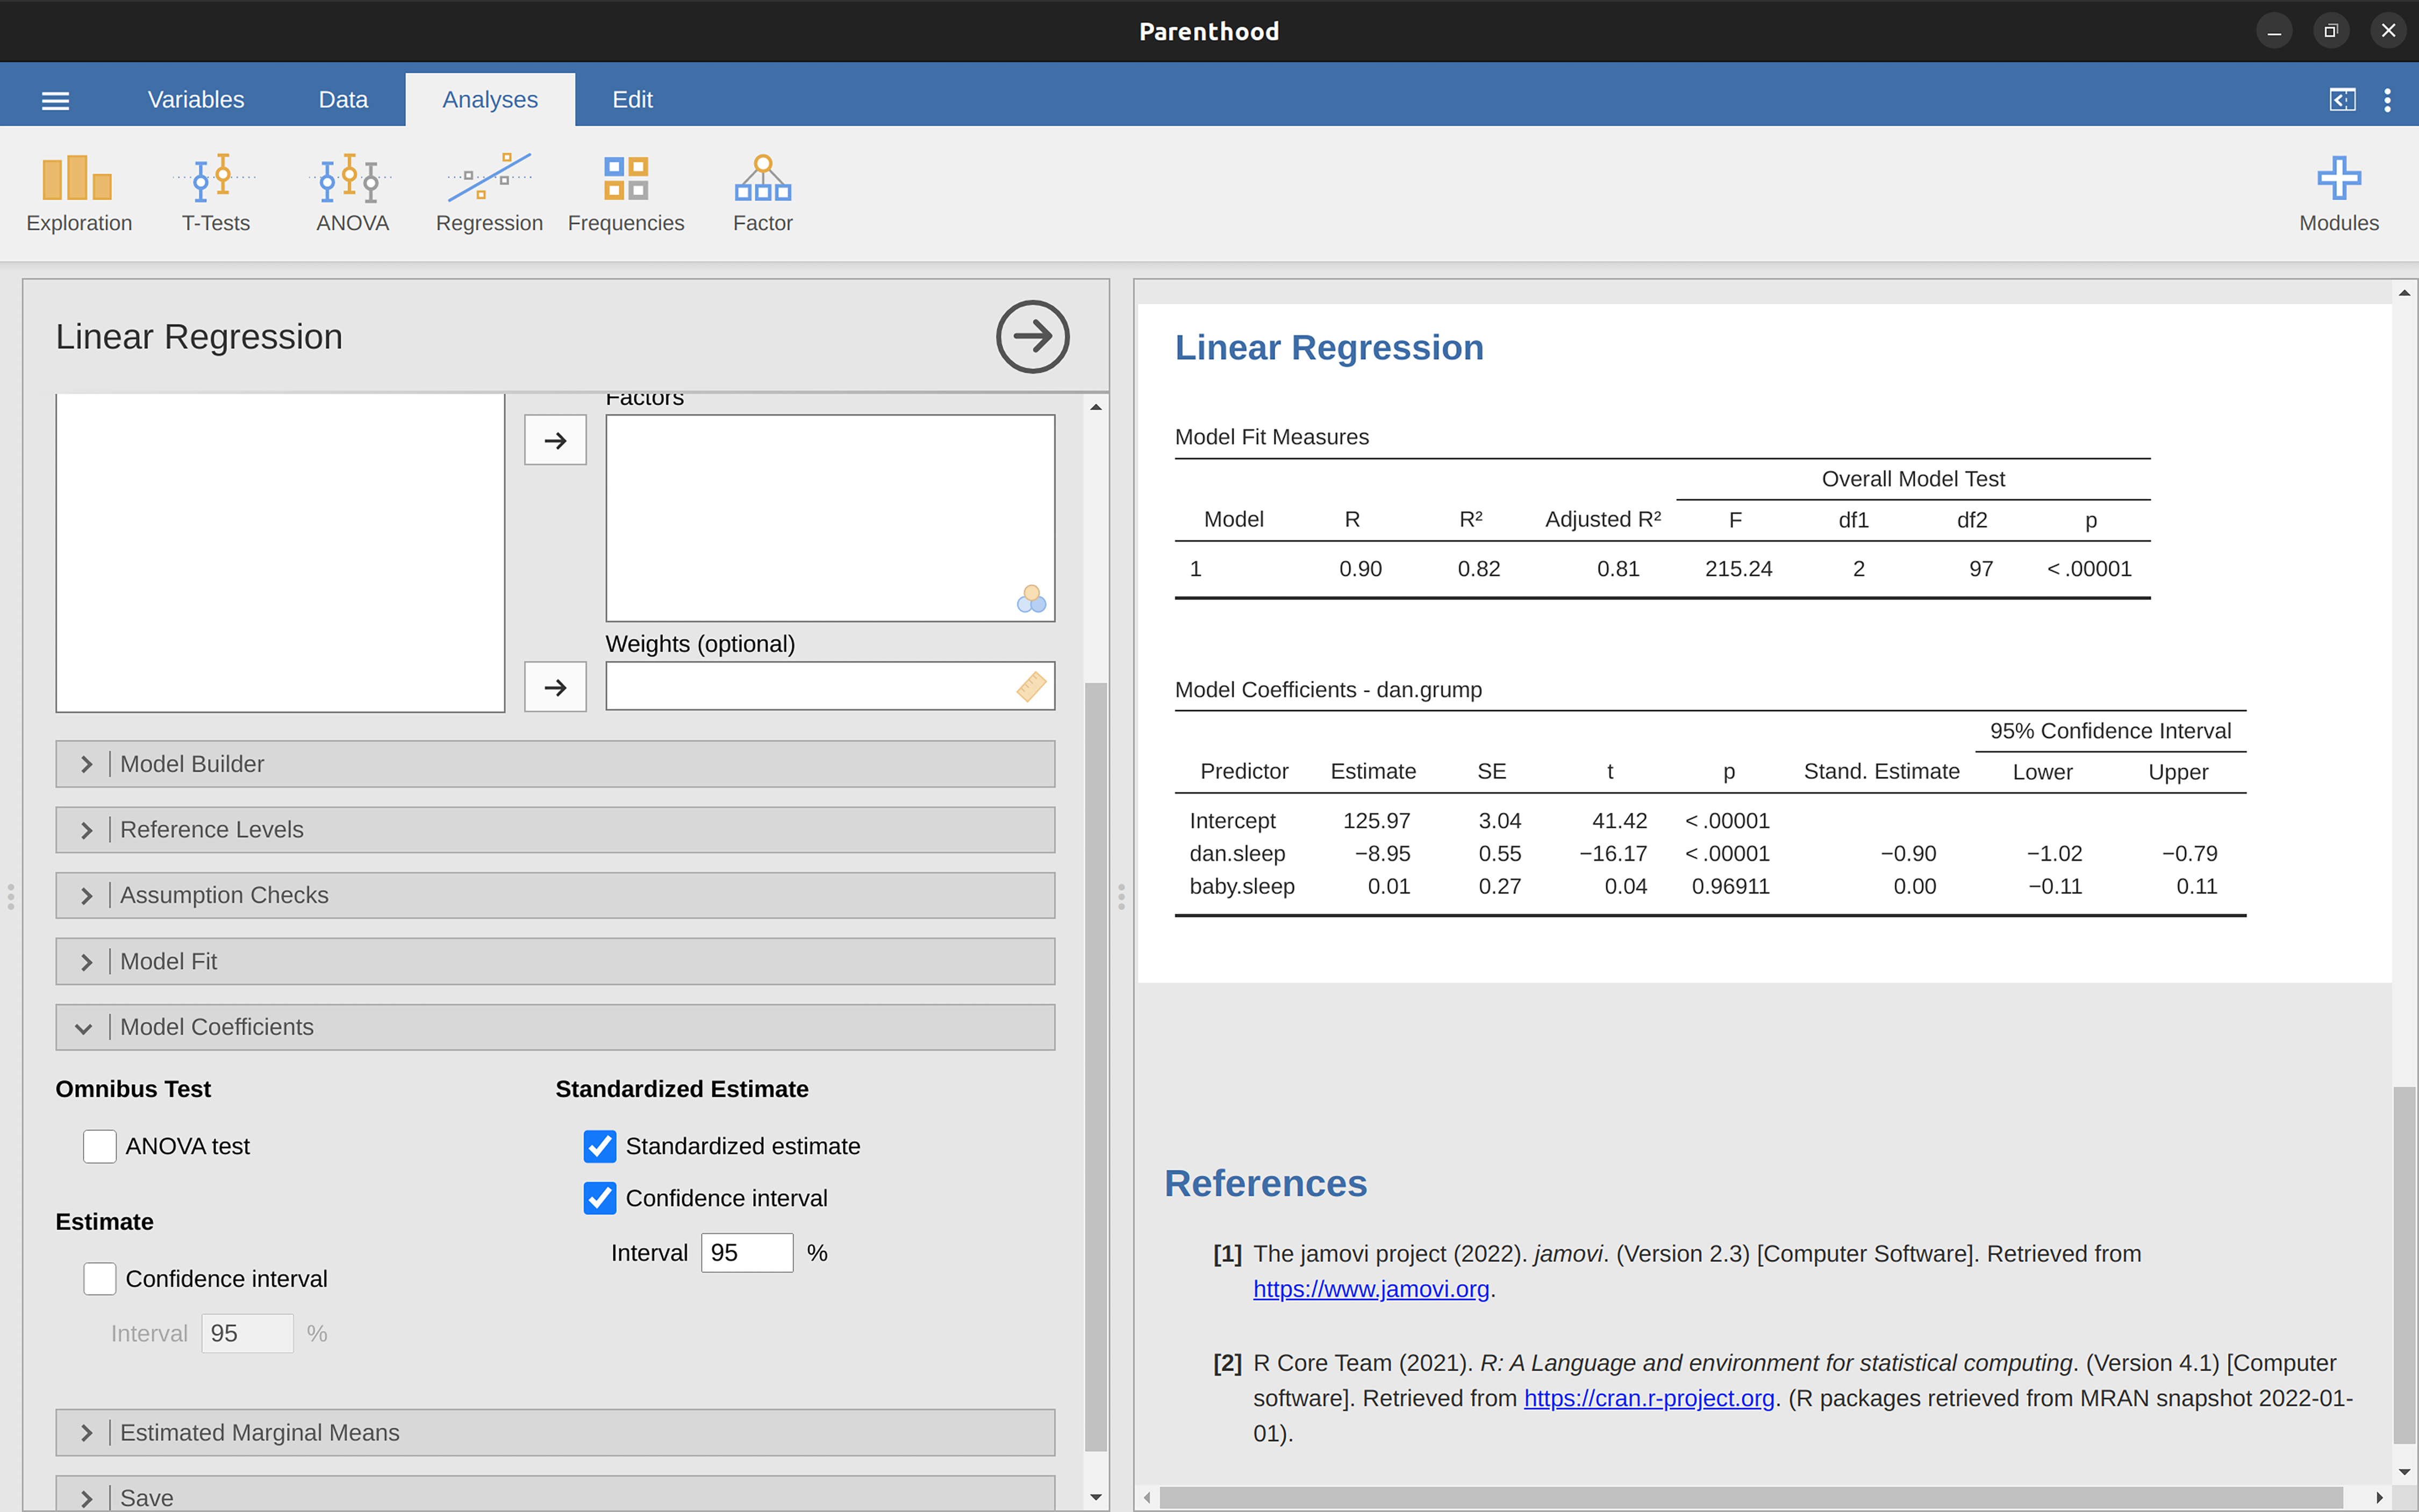
\includegraphics[width=1\textwidth,height=\textheight]{images/fig12-16.png} \hfill{}

\caption{\label{fig-fig12-16}Standardised coefficients, with 95\%
confidence intervals, for multiple linear regression}

\end{figure}

These results clearly show that the dani.sleep variable has a much
stronger effect than the baby.sleep variable. However, this is a perfect
example of a situation where it would probably make sense to use the
original coefficients b rather than the standardised coefficients
\(\beta\). After all, my sleep and the baby's sleep are already on the
same scale: number of hours slept. Why complicate matters by converting
these to \emph{z}-scores?

\hypertarget{assumptions-of-regression}{%
\section{Assumptions of regression}\label{assumptions-of-regression}}

The linear regression model that I've been discussing relies on several
assumptions. In \protect\hyperlink{sec-Model-checking}{Model checking}
we'll talk a lot more about how to check that these assumptions are
being met, but first let's have a look at each of them.

\begin{itemize}
\tightlist
\item
  \textbf{L}inearity. A pretty fundamental assumption of the linear
  regression model is that the relationship between \(X\) and \(Y\)
  actually is linear! Regardless of whether it's a simple regression or
  a multiple regression, we assume that the relationships involved are
  linear.
\item
  \textbf{I}ndependence: residuals are independent of each other. This
  is really just a ``catch all'' assumption, to the effect that
  ``there's nothing else funny going on in the residuals''. If there is
  something weird (e.g., the residuals all depend heavily on some other
  unmeasured variable) going on, it might screw things up. Independence
  isn't something that you can check directly and specifically with
  diagnostic tools, but if your regression diagnostics are messed up
  then think carefully about the independence of your observations and
  residuals.
\item
  \textbf{N}ormality. Like many of the models in statistics, basic
  simple or multiple linear regression relies on an assumption of
  normality. Specifically, it assumes that the residuals are normally
  distributed. It's actually okay if the predictors \(X\) and the
  outcome \(Y\) variables are non-normal, so long as the residuals
  \(\epsilon\) are normal. See the
  \protect\hyperlink{sec-Checking-the-normality-of-the-residuals}{Checking
  the normality of the residuals} section.
\item
  \textbf{E}quality (or ``homogeneity'') of variance. Strictly speaking,
  the regression model assumes that each residual \(\epsilon_i\) is
  generated from a normal distribution with mean 0, and (more
  importantly for the current purposes) with a standard deviation
  \(\sigma\) that is the same for every single residual. In practice,
  it's impossible to test the assumption that every residual is
  identically distributed. Instead, what we care about is that the
  standard deviation of the residual is the same for all values of
  \(\hat{Y}\), and (if we're being especially diligent) all values of
  every predictor \(X\) in the model.
\end{itemize}

So, we have four main assumptions for linear regression (that neatly
form the acronym \textbf{LINE}). And there are also a couple of other
things we should also check for:

\begin{itemize}
\tightlist
\item
  Uncorrelated predictors. The idea here is that, in a multiple
  regression model, you don't want your predictors to be too strongly
  correlated with each other. This isn't ``technically'' an assumption
  of the regression model, but in practice it's required. Predictors
  that are too strongly correlated with each other (referred to as
  ``collinearity'') can cause problems when evaluating the model. See
  \protect\hyperlink{checking-for-collinearity}{Checking for
  collinearity} section.
\item
  No ``bad'' outliers. Again, not actually a technical assumption of the
  model (or rather, it's sort of implied by all the others), but there
  is an implicit assumption that your regression model isn't being too
  strongly influenced by one or two anomalous data points because this
  raises questions about the adequacy of the model and the
  trustworthiness of the data in some cases. See the section on
  \protect\hyperlink{outliers-and-anomalous-data}{Outliers and anomalous
  data}.
\end{itemize}

\hypertarget{sec-Model-checking}{%
\section{Model checking}\label{sec-Model-checking}}

The main focus of this section is \textbf{regression diagnostics}, a
term that refers to the art of checking that the assumptions of your
regression model have been met, figuring out how to fix the model if the
assumptions are violated, and generally to check that nothing ``funny''
is going on. I refer to this as the ``art'' of model checking with good
reason. It's not easy, and while there are a lot of easily available
tools that you can use to diagnose and maybe even cure the problems that
affect your model (if there are any, that is!), you really do need to
exercise a certain amount of judgement when doing this.

In this section I describe several different things you can do to check
that your regression model is doing what it's supposed to. It doesn't
cover the full space of things you could do, but it's still much more
detailed than what is often done in practice -- unfortunately! But it's
important that you get a sense of what tools are at your disposal, so
I'll try to introduce a bunch of them here. Finally, I should note that
this section draws quite heavily from Fox \& Weisberg (2011), the book
associated with the ``car'' package that is used to conduct regression
analysis in \(R\). The ``car'' package is notable for providing some
excellent tools for regression diagnostics, and the book itself talks
about them in an admirably clear fashion. I don't want to sound too
gushy about it, but I do think that Fox \& Weisberg (2011) is well worth
reading, even if some of the advanced diagnostic techniques are only
available in ``R'' and not jamovi.

\hypertarget{three-kinds-of-residuals}{%
\subsection{Three kinds of residuals}\label{three-kinds-of-residuals}}

The majority of regression diagnostics revolve around looking at the
residuals, and there are several different kinds of residual that we
might consider. In particular, the following three kinds of residuals
are referred to in this section: ``ordinary residuals'', ``standardised
residuals'', and ``Studentised residuals''. There is a fourth kind that
you'll see referred to in some of the Figures, and that's the ``Pearson
residual''. However, for the models that we're talking about in this
chapter the Pearson residual is identical to the ordinary residual.

The first and simplest kind of residuals that we care about are
\textbf{ordinary residuals}. These are the actual raw residuals that
I've been talking about throughout this chapter so far. The ordinary
residual is just the difference between the predicted value
\(\hat{Y}_i\) and the observed value \(Y_i\). I've been using the
notation \(\epsilon_i\) to refer to the i-th ordinary residual and so,
with this in mind, we have the very simple equation:
\[\epsilon_i=Y_i-\hat{Y_i}\]

This is of course what we saw earlier, and unless I specifically refer
to some other kind of residual, this is the one I'm talking about. So
there's nothing new here. I just wanted to repeat myself. One drawback
to using ordinary residuals is that they're always on a different scale,
depending on what the outcome variable is and how good the regression
model is. That is, unless you've decided to run a regression model
without an intercept term, the ordinary residuals will have mean 0 but
the variance is different for every regression. In a lot of contexts,
especially where you're only interested in the pattern of the residuals
and not their actual values, it's convenient to estimate the
\textbf{standardised residuals}, which are normalised in such a way as
to have a standard deviation of 1.

{[}Additional technical detail\footnote{The way we calculate these is to
  divide the ordinary residual by an estimate of the (population)
  standard deviation of these residuals. For technical reasons, the
  formula for this is:
  \[\epsilon_i^{'}=\frac{\epsilon_i}{\hat{\sigma}\sqrt{1-h_i}}\] where
  \(\hat{\sigma}\) in this context is the estimated population standard
  deviation of the ordinary residuals, and \(h_i\) is the ``hat value''
  of the \(i\)th observation. I haven't explained hat values to you yet,
  so this won't make a lot of sense. For now, it's enough to interpret
  the standardised residuals as if we'd converted the ordinary residuals
  to \emph{z}-scores.}{]}

The third kind of residuals are \textbf{Studentised residuals} (also
called ``jackknifed residuals'') and they're even fancier than
standardised residuals. Again, the idea is to take the ordinary residual
and divide it by some quantity in order to estimate some standardised
notion of the residual.\footnote{The formula for doing the calculations
  this time is subtly different
  \(\epsilon _i^*=\frac{\epsilon_i}{\hat{\sigma}_{(-i)}\sqrt{1-h_i}}\)
  Notice that our estimate of the standard deviation here is written
  \(\hat{\sigma}_{(-i)}\). What this corresponds to is the estimate of
  the residual standard deviation that you would have obtained if you
  just deleted the \(i\)th observation from the data set. This sounds
  like the sort of thing that would be a nightmare to calculate, since
  it seems to be saying that you have to run \(N\) new regression models
  (even a modern computer might grumble a bit at that, especially if
  you've got a large data set). Fortunately, this standard deviation
  estimate is actually given by the following equation:
  \(\hat{\sigma}_{(-i)}= \hat{\sigma}\sqrt{\frac{N-K-1-{\epsilon_i^{'}}^2}{N-K-2}}\).}

Before moving on, I should point out that you don't often need to obtain
these residuals yourself, even though they are at the heart of almost
all regression diagnostics. Most of the time the various options that
provide the diagnostics, or assumption checks, will take care of these
calculations for you. Even so, it's always nice to know how to actually
get hold of these things yourself in case you ever need to do something
non-standard.

\hypertarget{checking-the-linearity-of-the-relationship}{%
\subsection{Checking the linearity of the
relationship}\label{checking-the-linearity-of-the-relationship}}

We should check for the linearity of the relationships between the
predictors and the outcomes. There's a few different things that you
might want to do in order to check this. Firstly, it never hurts to just
plot the relationship between the predicted values \(\hat{Y}_i\) and the
observed values \(Y_i\) for the outcome variable, as illustrated in
Figure~\ref{fig-fig12-17}. To draw this in jamovi we saved the predicted
values to the data set, and then drew a scatterplot of the observed
against the predicted (fitted) values. This gives you a kind of ``big
picture view'' -- if this plot looks approximately linear, then we're
probably not doing too badly (though that's not to say that there aren't
problems). However, if you can see big departures from linearity here,
then it strongly suggests that you need to make some changes.

\begin{figure}[h!]


\includegraphics[width=0.8\textwidth,height=\textheight]{images/fig12-17.png} \hfill{}

\caption{\label{fig-fig12-17}jamovi plot of the predicted values against
the observed values of the outcome variable. A straight(-ish) line is
what we are hoping to see here. This looks pretty good, suggesting that
there is nothing grossly wrong}

\end{figure}

In any case, in order to get a more detailed picture it's often more
informative to look at the relationship between the predicted values and
the residuals themselves. Again, in jamovi you can save the residuals to
the data set and then draw a scatterplot of the predicted values against
the residual values, as in Figure~\ref{fig-fig12-18}. As you can see,
not only does it draw the scatterplot showing the predicted value
against the residuals, you can also plot a line through the data that
shows the relationship between the two. Ideally, this should be a
straight, perfectly horizontal line. In practice, we're looking for a
reasonably straight or flat line. This is a matter of judgement.

\begin{figure}[h!]


\includegraphics[width=0.8\textwidth,height=\textheight]{images/fig12-18.png} \hfill{}

\caption{\label{fig-fig12-18}jamovi plot of the predicted values against
the residuals, with a line showing the relationship between the two. If
this is horizontal and straight(-ish), then we can feel reasonably
confident that the ``average residual'' for all ``predicted values'' is
more or less the same.}

\end{figure}

More advanced versions of the same plot are produced by checking
`Residuals plots' in the regression analysis `Assumption checks' options
in jamovi. These are useful for checking linearity, normality and
equality of variance assumptions, and we look at these in more detail in
Section~\ref{sec-Checking-the-normality-of-the-residuals}. This option
not only draws plots comparing the predicted values to the residuals, it
does so for each individual predictor.

\hypertarget{sec-Checking-the-normality-of-the-residuals}{%
\subsection{Checking the normality of the
residuals}\label{sec-Checking-the-normality-of-the-residuals}}

Like many of the statistical tools we've discussed in this book,
regression models rely on a normality assumption. In this case, we
assume that the residuals are normally distributed. The first thing we
can do is draw a QQ-plot via the `Assumption Checks' -- `Assumption
Checks' -- `Q-Q plot of residuals' option. The output is shown in
Figure~\ref{fig-fig12-19}, showing the standardised residuals plotted as
a function of their theoretical quantiles according to the regression
model.

Another thing we should check is the relationship between the predicted
(fitted) values and the residuals themselves. We can get jamovi to do
this using the `Residuals Plots' option, which provides a scatterplot
for each predictor variable, the outcome variable, and the predicted
values against residuals, see Figure~\ref{fig-fig12-20}. In these plots
we are looking for a fairly uniform distribution of dots, with no clear
bunching or patterning of the dots. Looking at these plots, there is
nothing particularly worrying as the dots are fairly evenly spread
across the whole plot. There may be a little bit of non-uniformity in
plot (b), but it is not a strong deviation and probably not worth
worrying about.

\begin{figure}[H]

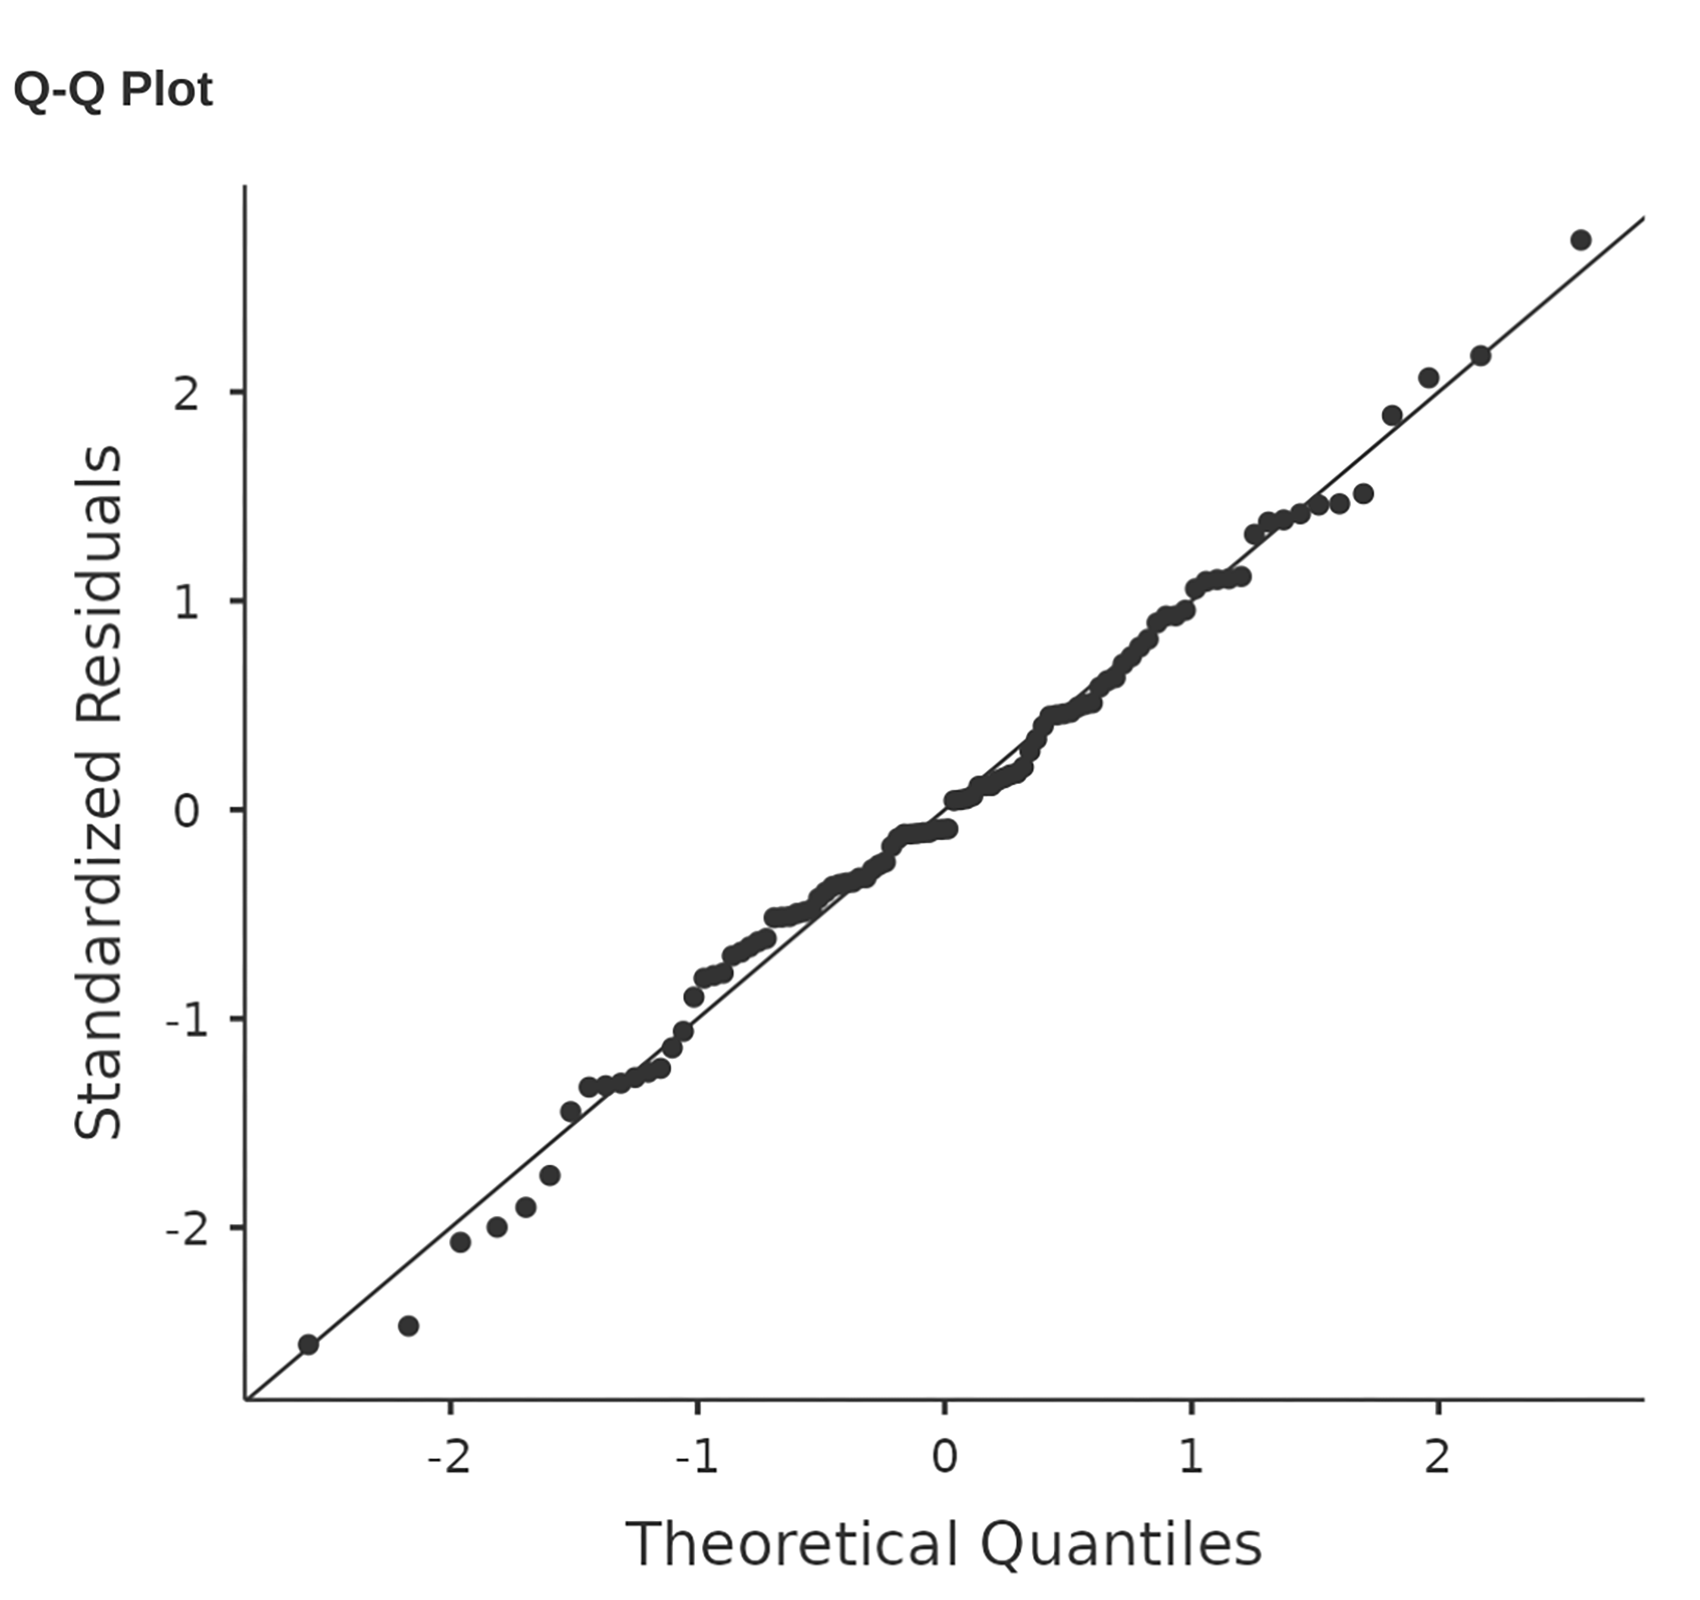
\includegraphics[width=0.7\textwidth,height=\textheight]{images/fig12-19.png} \hfill{}

\caption{\label{fig-fig12-19}Plot of the theoretical quantiles according
to the model, against the quantiles of the standardised residuals,
produced in jamovi}

\end{figure}

\begin{figure}[H]

\begin{minipage}[t]{\linewidth}

{\centering 


\includegraphics[width=0.45\textwidth,height=\textheight]{images/fig12-20a.png}
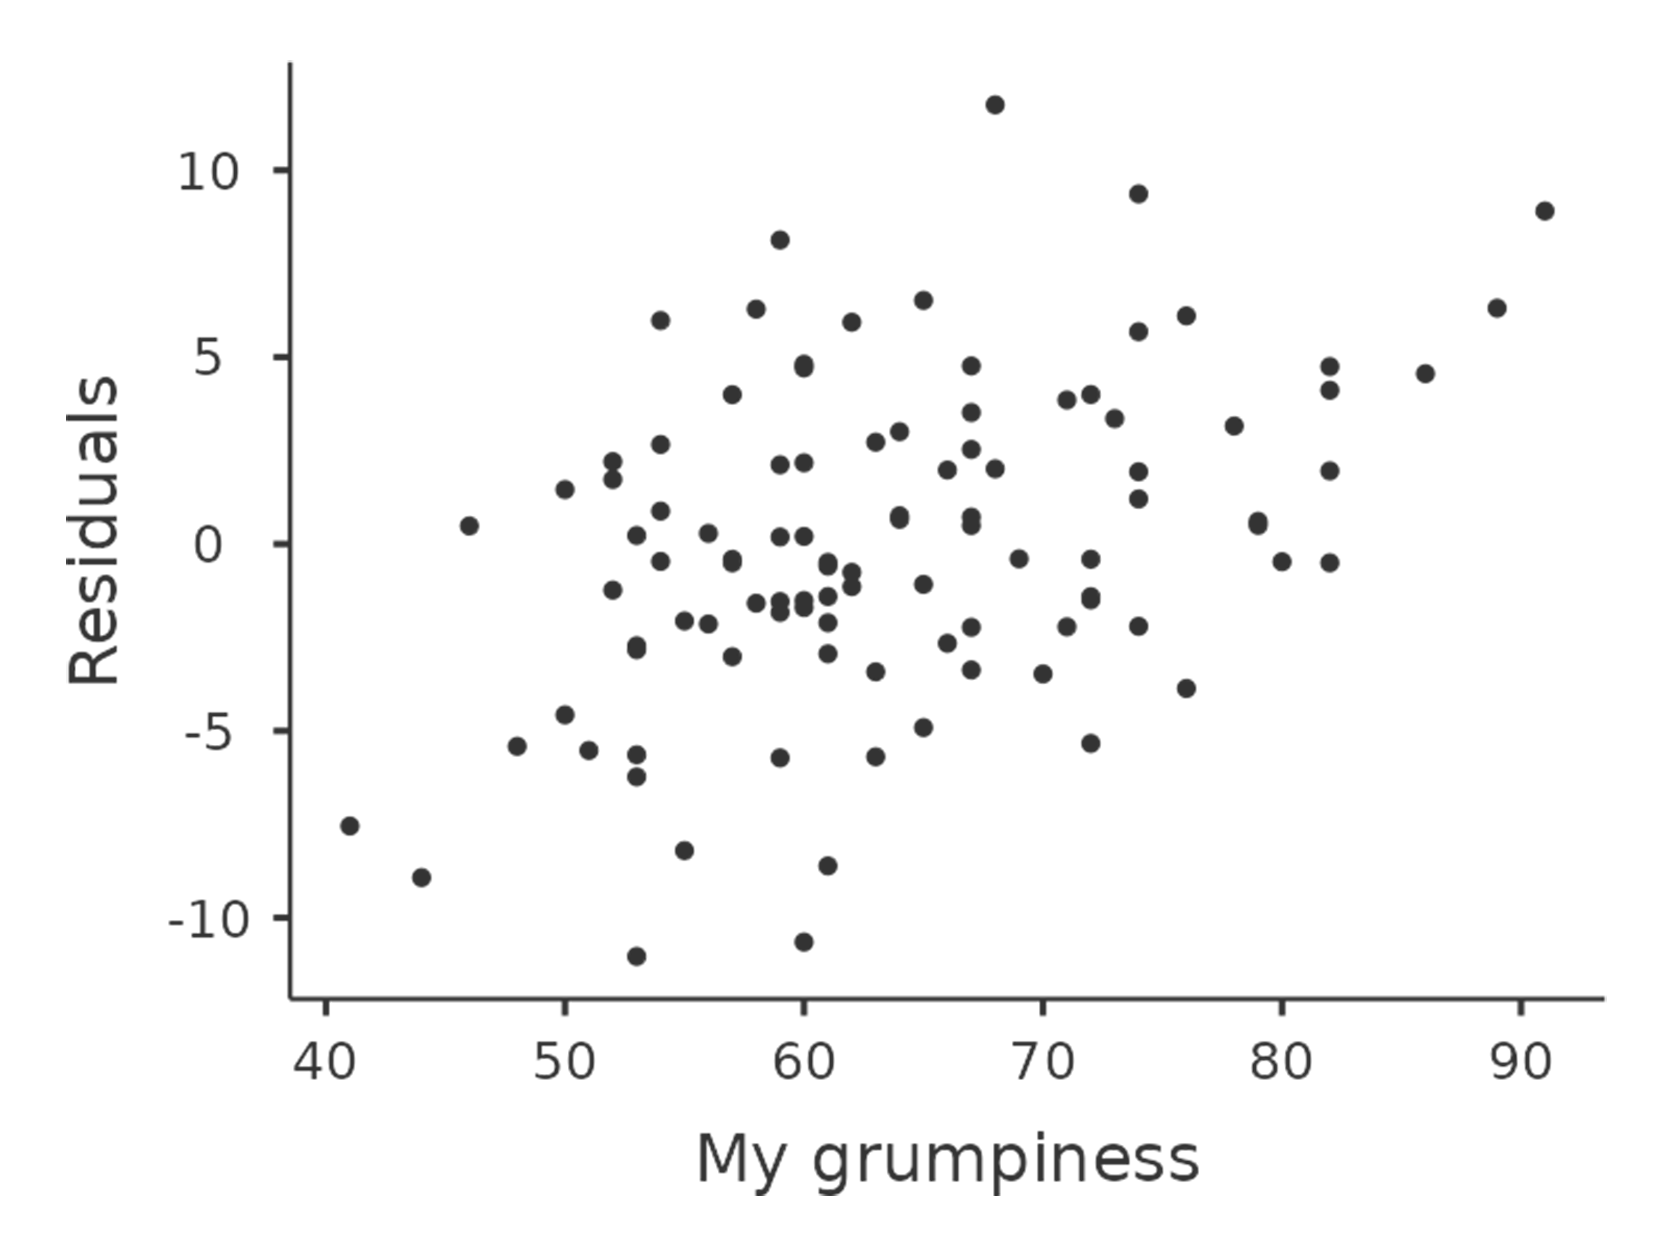
\includegraphics[width=0.45\textwidth,height=\textheight]{images/fig12-20b.png}

\includegraphics[width=0.45\textwidth,height=\textheight]{images/fig12-20c.png}

\includegraphics[width=0.45\textwidth,height=\textheight]{images/fig12-20d.png}

}

\end{minipage}%

\caption{\label{fig-fig12-20}Residuals plots produced in jamovi}

\end{figure}

If we were worried, then in a lot of cases the solution to this problem
(and many others) is to transform one or more of the variables. We
discussed the basics of variable transformation in
\textbf{?@sec-Transforming-and-recoding-a-variable}, but I do want to
make special note of one additional possibility that I didn't explain
fully earlier: the Box-Cox transform. The Box-Cox function is a fairly
simple one and it's very widely used.\footnote{\(f(x,\lambda)=\frac{x^{\lambda}-1}{\lambda}\)
  for all values of \(\lambda\) except \(\lambda = 0\). When
  \(\lambda = 0\) we just take the natural logarithm (i.e., ln(\(x\)).}

You can calculate it using the BOXCOX function in the `Compute'
variables screen in jamovi.

\hypertarget{checking-equality-of-variance}{%
\subsection{Checking equality of
variance}\label{checking-equality-of-variance}}

The regression models that we've talked about all make an equality
(i.e.homogeneity) of variance assumption: the variance of the residuals
is assumed to be constant. To plot this in jamovi first we need to
calculate the square root of the (absolute) size of the
residual\footnote{In jamovi, you can compute this new variable using the
  formula `SQRT(ABS(Residuals))'.} and then plot this against the
predicted values, as in Figure~\ref{fig-fig12-21}. Note that this plot
actually uses the standardised residuals rather than the raw ones, but
it's immaterial from our point of view. What we're looking to see here
is a straight, horizontal line running through the middle of the
plot.\footnote{It's a bit beyond the scope of this chapter to talk about
  how to deal with violations of homogeneity of variance, but I'll give
  you a quick sense of what you need to consider. The \textbf{main}
  thing to worry about, if homogeneity of variance is violated, is that
  the standard error estimates associated with the regression
  coefficients are no longer entirely reliable, and so your \(t\)-tests
  for the coefficients aren't quite right either. A simple fix to the
  problem is to make use of a ``heteroscedasticity corrected covariance
  matrix'' when estimating the standard errors. These are often called
  \textbf{\emph{sandwich estimators}}, and these can be estimated in
  \(R\) (but not directly in jamovi).}

\begin{figure}[h!]


\includegraphics[width=0.8\textwidth,height=\textheight]{images/fig12-21.png} \hfill{}

\caption{\label{fig-fig12-21}jamovi plot of the predicted values (model
predictions) against the square root of the absolute standardised
residuals. This plot is used to diagnose violations of homogeneity of
variance. If the variance is really constant, then the line through the
middle should be horizontal and flat(-ish).}

\end{figure}

\hypertarget{checking-for-collinearity}{%
\subsection{Checking for collinearity}\label{checking-for-collinearity}}

Another regression diagnostic is provided by \textbf{variance inflation
factors} (VIFs), which are useful for determining whether or not the
predictors in your regression model are too highly correlated with each
other. There is a variance inflation factor associated with each
predictor \(X_k\) in the model.\footnote{The formula for the \(k\)-th
  VIF is: \(VIF_k=\frac{1}{1-R^2_{(-k)}}\) where \(R^2_{(-k)}\) refers
  to R-squared value you would get if you ran a regression using \(X_k\)
  as the outcome variable, and all the other \(X\) variables as the
  predictors. The idea here is that \(R^2_{(-k)}\) is a very good
  measure of the extent to which \(X_k\) is correlated with all the
  other variables in the model. Better yet, the square root of the VIF
  is pretty interpretable: it tells you how much wider the confidence
  interval for the corresponding coefficient \(b_k\) is, relative to
  what you would have expected if the predictors are all nice and
  uncorrelated with one another.}

If you've only got two predictors, the VIF values are always going to be
the same, as we can see if we click on the `Collinearity' checkbox in
the `Regression' -- `Assumptions' options in jamovi. For both dani.sleep
and baby.sleep the VIF is \(1.65\). And since the square root of
\(1.65\) is \(1.28\), we see that the correlation between our two
predictors isn't causing much of a problem.

To give a sense of how we could end up with a model that has bigger
collinearity problems, suppose I were to run a much less interesting
regression model, in which I tried to predict the day on which the data
were collected, as a function of all the other variables in the data
set. To see why this would be a bit of a problem, let's have a look at
the correlation matrix for all four variables
(Figure~\ref{fig-fig12-22}).

\begin{figure}[h!]

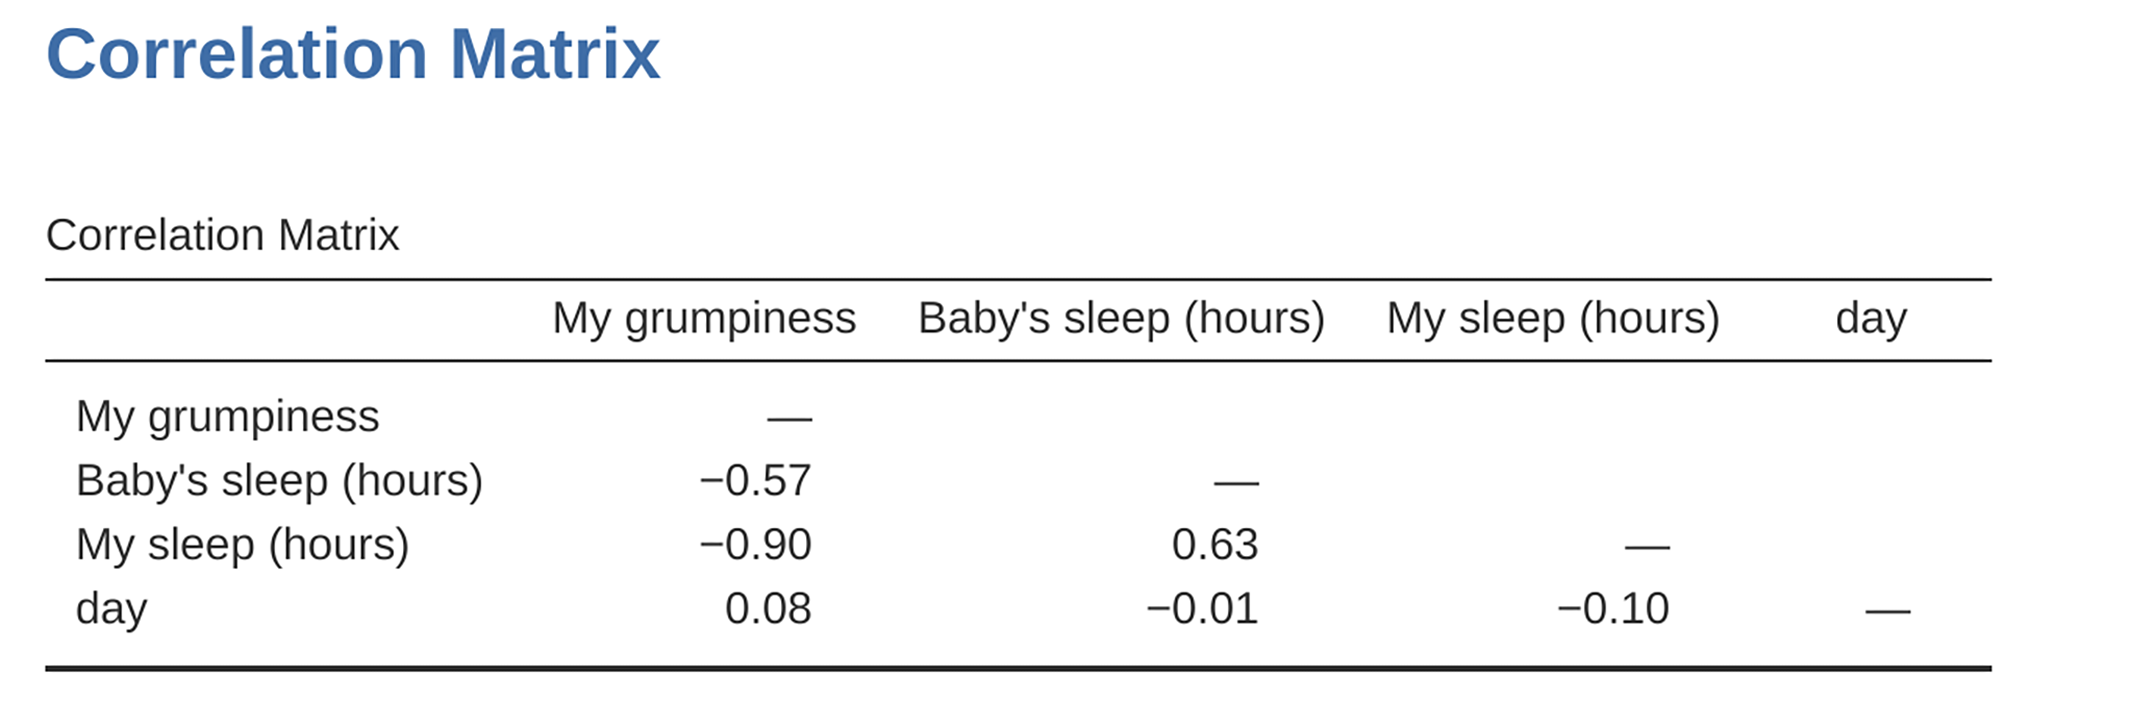
\includegraphics[width=1\textwidth,height=\textheight]{images/fig12-22.png} \hfill{}

\caption{\label{fig-fig12-22}Correlation matrix in jamovi for all four
variables}

\end{figure}

We have some fairly large correlations between some of our predictor
variables! When we run the regression model and look at the VIF values,
we see that the collinearity is causing a lot of uncertainty about the
coefficients. First, run the regression, as in Figure~\ref{fig-fig12-23}
and you can see from the VIF values that, yep, that's some mighty fine
collinearity there.

\begin{figure}[h!]

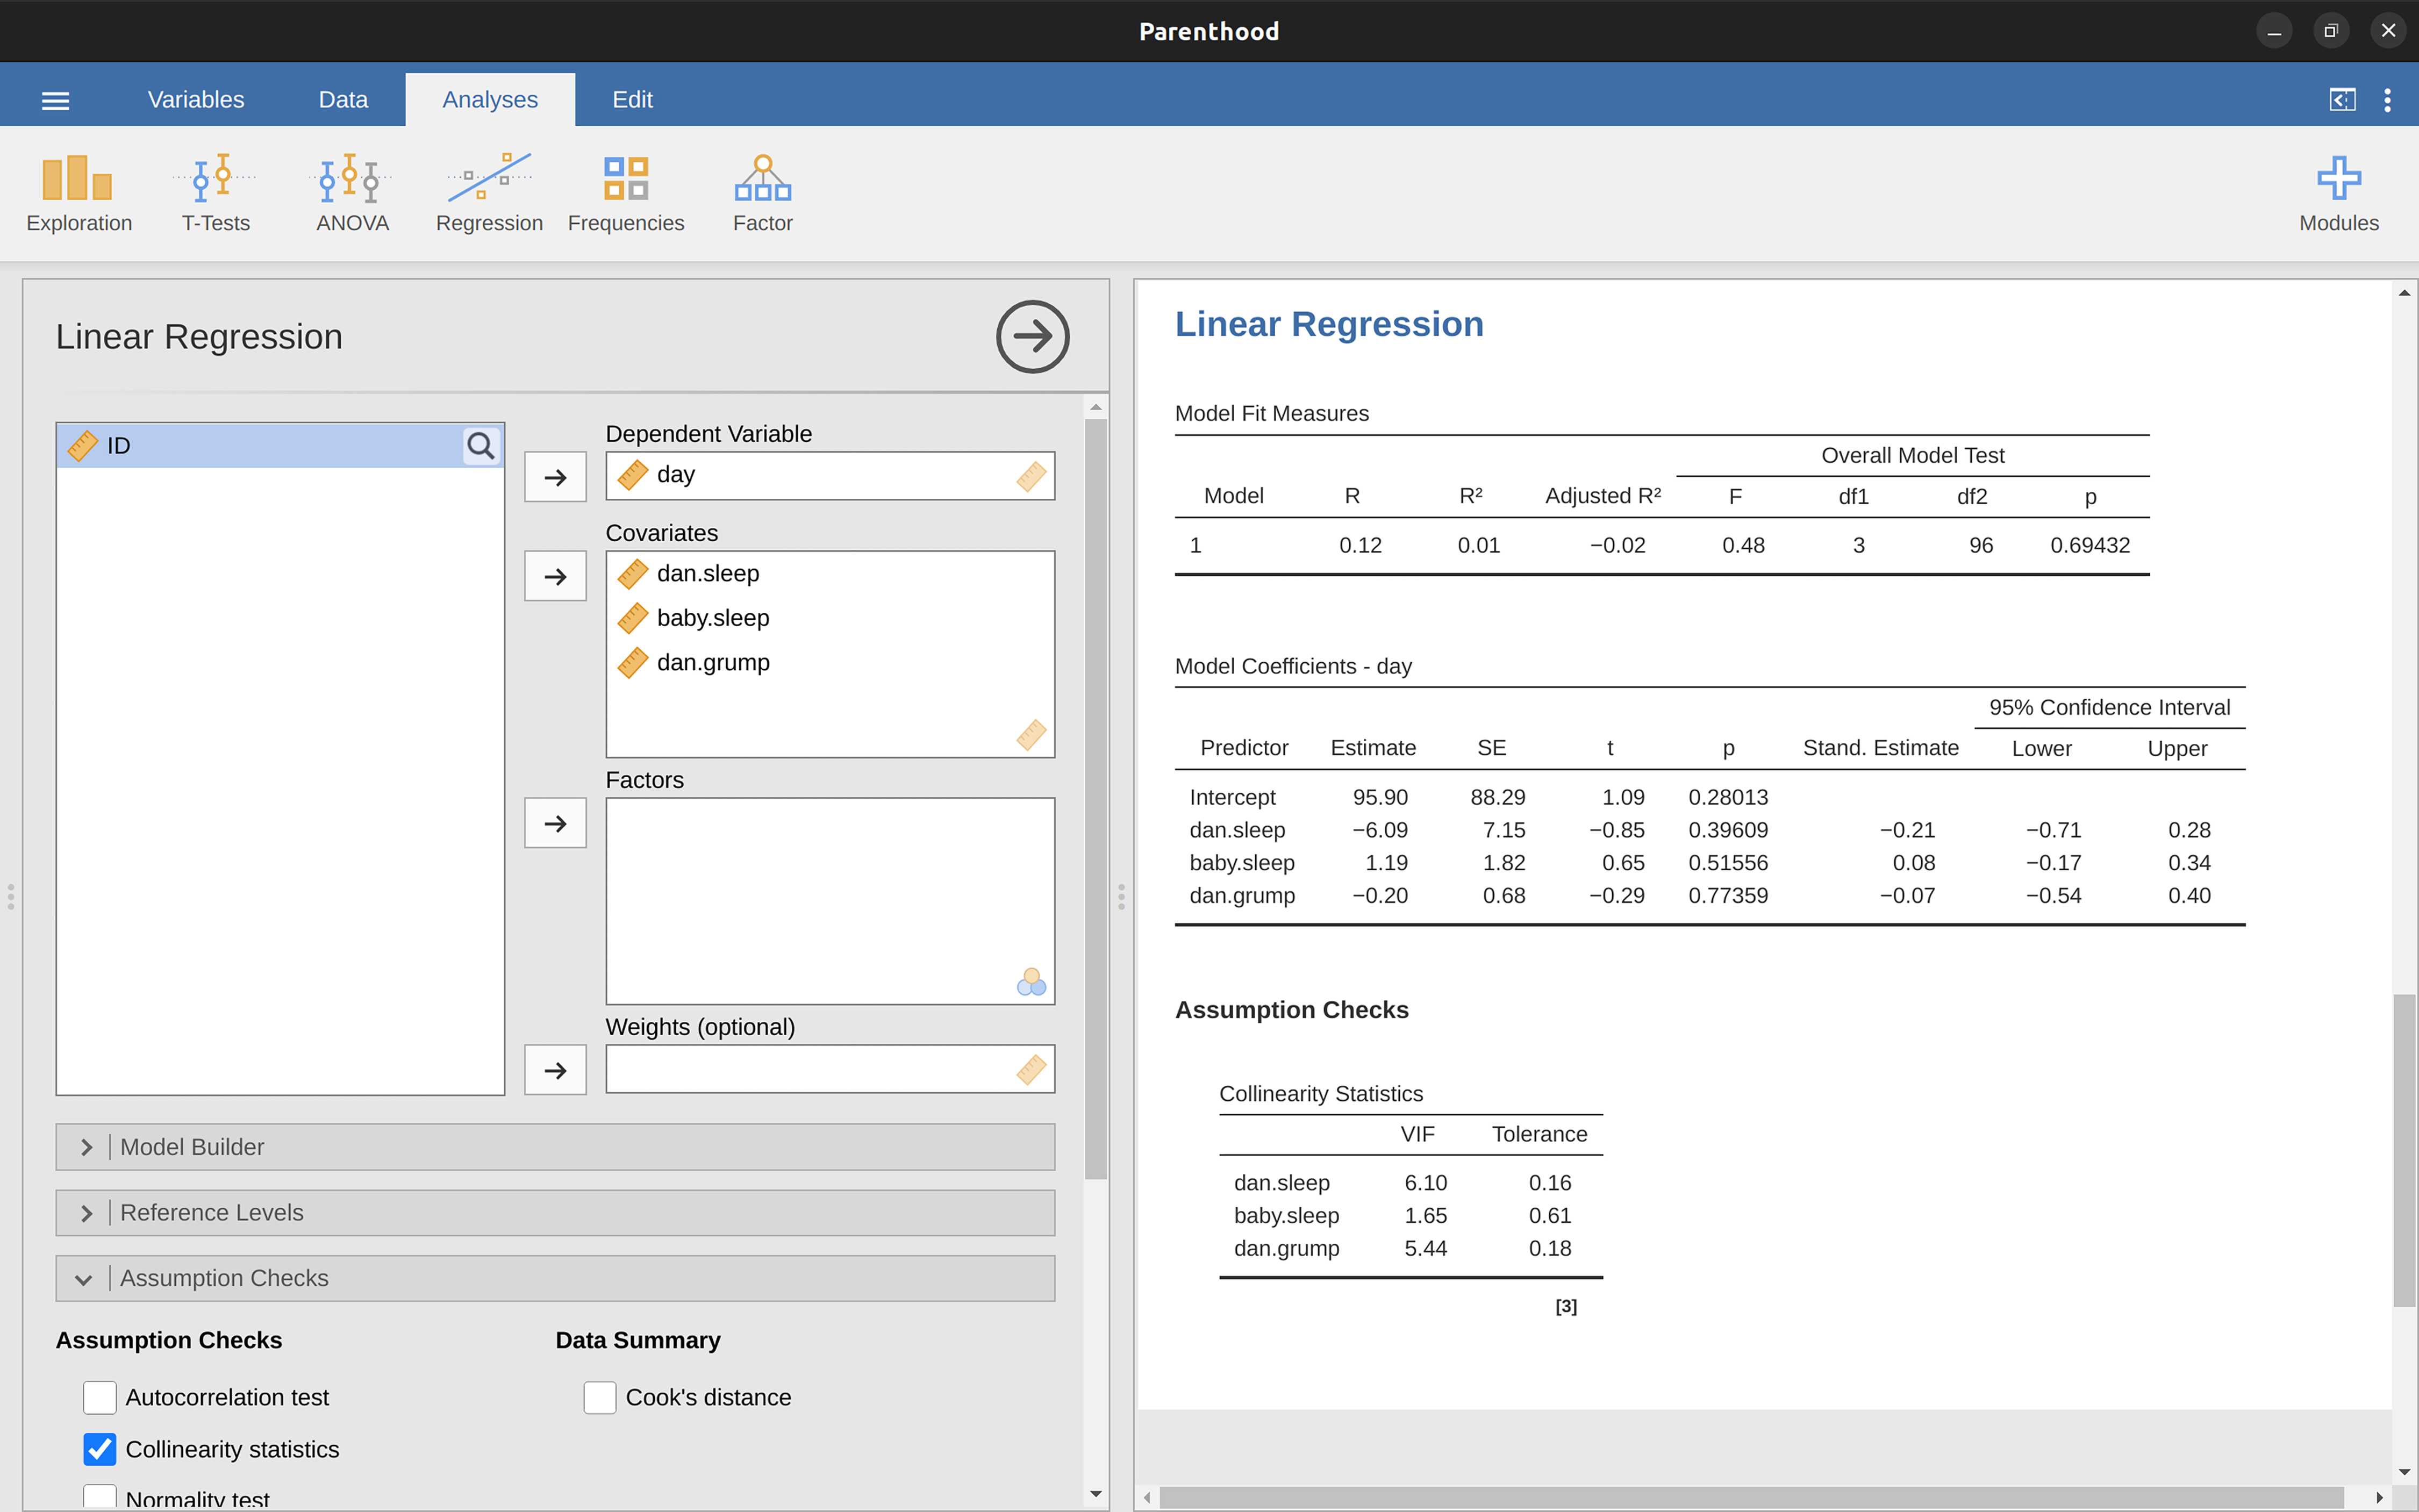
\includegraphics[width=0.99\textwidth,height=\textheight]{images/fig12-23.png} \hfill{}

\caption{\label{fig-fig12-23}Collinearity statistics for multiple
regression, produced in jamovi}

\end{figure}

\begin{figure}[h!]

\includegraphics[width=0.8\textwidth,height=\textheight]{12-Correlation-and-linear-regression_files/figure-pdf/fig-fig12-24-1.pdf} \hfill{}

\caption{\label{fig-fig12-24}An illustration of outliers. The solid line
shows the regression line with the anomalous outlier observation
included. The dashed line plots the regression line estimated without
the anomalous outlier observation included. The vertical line from the
outlier point to the dashed regression line illustrates the large
residual error for the outlier}

\end{figure}

\hypertarget{outliers-and-anomalous-data}{%
\subsection{Outliers and anomalous
data}\label{outliers-and-anomalous-data}}

One danger that you can run into with linear regression models is that
your analysis might be disproportionately sensitive to a smallish number
of ``unusual'' or ``anomalous'' observations. I discussed this idea
previously in \textbf{?@sec-Using-box-plots-to-detect-outliers} in the
context of discussing the outliers that get automatically identified by
the boxplot option under `Exploration' -- `Descriptives', but this time
we need to be much more precise. In the context of linear regression,
there are three conceptually distinct ways in which an observation might
be called ``anomalous''. All three are interesting, but they have rather
different implications for your analysis.

The first kind of unusual observation is an \textbf{outlier}. The
definition of an outlier (in this context) is an observation that is
very different from what the regression model predicts. An example is
shown in Figure~\ref{fig-fig12-24}, the outlier has an unusual value on
the outcome (y-axis location), but not the predictor (x-axis location)
and lies a long way from the regression line. In practice, we
operationalise this concept by saying that an outlier is an observation
that has a very large residual, \(\epsilon_i^*\).

Outliers are interesting: a big outlier might correspond to junk data,
e.g., the variables might have been recorded incorrectly in the data
set, or some other defect may be detectable. Note that you shouldn't
throw an observation away just because it's an outlier. But the fact
that it's an outlier is often a cue to look more closely at that case
and try to find out why it's so different.

\begin{figure}[h!]

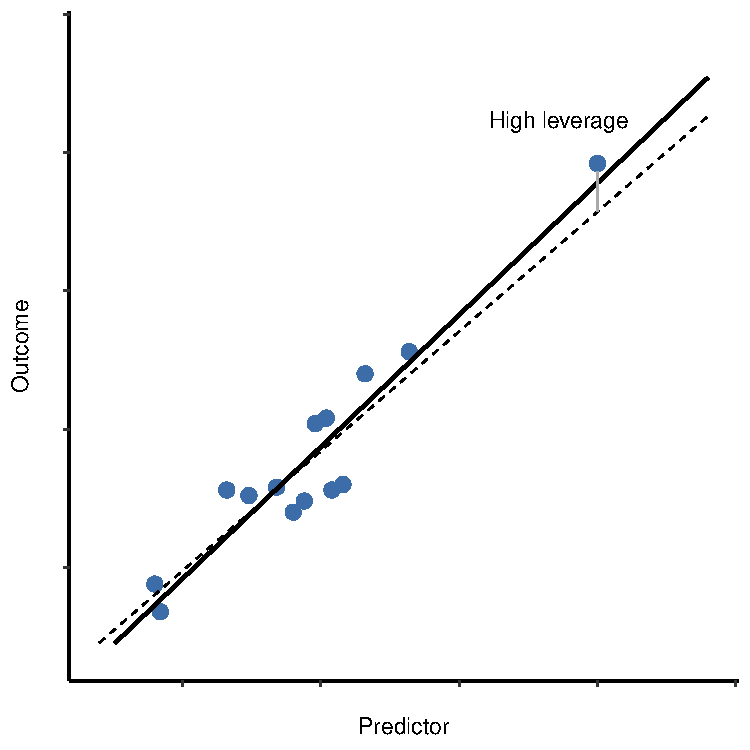
\includegraphics[width=0.8\textwidth,height=\textheight]{12-Correlation-and-linear-regression_files/figure-pdf/fig-fig12-25-1.pdf} \hfill{}

\caption{\label{fig-fig12-25}An illustration of high leverage points.
The anomalous observation in this case is unusual both in terms of the
predictor (x-axis) and the outcome (y-axis), but this unusualness is
highly consistent with the pattern of correlations that exists among the
other observations. The observation falls very close to the regression
line and does not distort it by very much}

\end{figure}

The second way in which an observation can be unusual is if it has high
\textbf{leverage}, which happens when the observation is very different
from all the other observations. This doesn't necessarily have to
correspond to a large residual. If the observation happens to be unusual
on all variables in precisely the same way, it can actually lie very
close to the regression line. An example of this is shown in
Figure~\ref{fig-fig12-25}. The leverage of an observation is
operationalised in terms of its hat value, usually written \(h_i\). The
formula for the hat value is rather complicated\footnote{Again, for the
  linear algebra fanatics: the ``hat matrix'' is defined to be that
  matrix \(H\) that converts the vector of observed values \(y\) into a
  vector of predicted values \(\hat{y}\), such that \(\hat{y} = Hy\).
  The name comes from the fact that this is the matrix that ``puts a hat
  on y''. The hat value of the i-th observation is the i-th diagonal
  element of this matrix (so technically I should be writing it as
  \(h_{ii}\) rather than \(h_i\)). And here's how it's calculated:
  \(H = X(X^{'}X)^{1}X^{'}\).} but its interpretation is not: \(h_i\) is
a measure of the extent to which the i-th observation is ``in control''
of where the regression line ends up going.

In general, if an observation lies far away from the other ones in terms
of the predictor variables, it will have a large hat value (as a rough
guide, high leverage is when the hat value is more than 2-3 times the
average; and note that the sum of the hat values is constrained to be
equal to \(K + 1\)). High leverage points are also worth looking at in
more detail, but they're much less likely to be a cause for concern
unless they are also outliers.

This brings us to our third measure of unusualness, the
\textbf{influence} of an observation. A high influence observation is an
outlier that has high leverage. That is, it is an observation that is
very different to all the other ones in some respect, and also lies a
long way from the regression line. This is illustrated in
Figure~\ref{fig-fig12-26}. Notice the contrast to the previous two
figures. Outliers don't move the regression line much and neither do
high leverage points. But something that is both an outlier and has high
leverage, well that has a big effect on the regression line. That's why
we call these points high influence, and it's why they're the biggest
worry. We operationalise influence in terms of a measure known as
\textbf{Cook's distance}.\footnote{\(D_i=\frac{{\epsilon_i^*}^2}{K+1} \times \frac{h_i}{1-h_i}\)
  Notice that this is a multiplication of something that measures the
  outlier-ness of the observation (the bit on the left), and something
  that measures the leverage of the observation (the bit on the right).}

\begin{figure}[h!]

\includegraphics[width=0.9\textwidth,height=\textheight]{12-Correlation-and-linear-regression_files/figure-pdf/fig-fig12-26-1.pdf} \hfill{}

\caption{\label{fig-fig12-26}An illustration of high influence points.
In this case, the anomalous observation is highly unusual on the
predictor variable (x-axis), and falls a long way from the regression
line. As a consequence, the regression line is highly distorted, even
though (in this case) the anomalous observation is entirely typical in
terms of the outcome variable (y-axis)}

\end{figure}

In order to have a large Cook's distance an observation must be a fairly
substantial outlier and have high leverage. As a rough guide, Cook's
distance greater than 1 is often considered large (that's what I
typically use as a quick and dirty rule).

In jamovi, information about Cook's distance can be calculated by
clicking on the `Cook's Distance' checkbox in the `Assumption Checks' --
`Data Summary' options. When you do this, for the multiple regression
model we have been using as an example in this chapter, you get the
results as shown in Figure~\ref{fig-fig12-27}.

\begin{figure}[H]

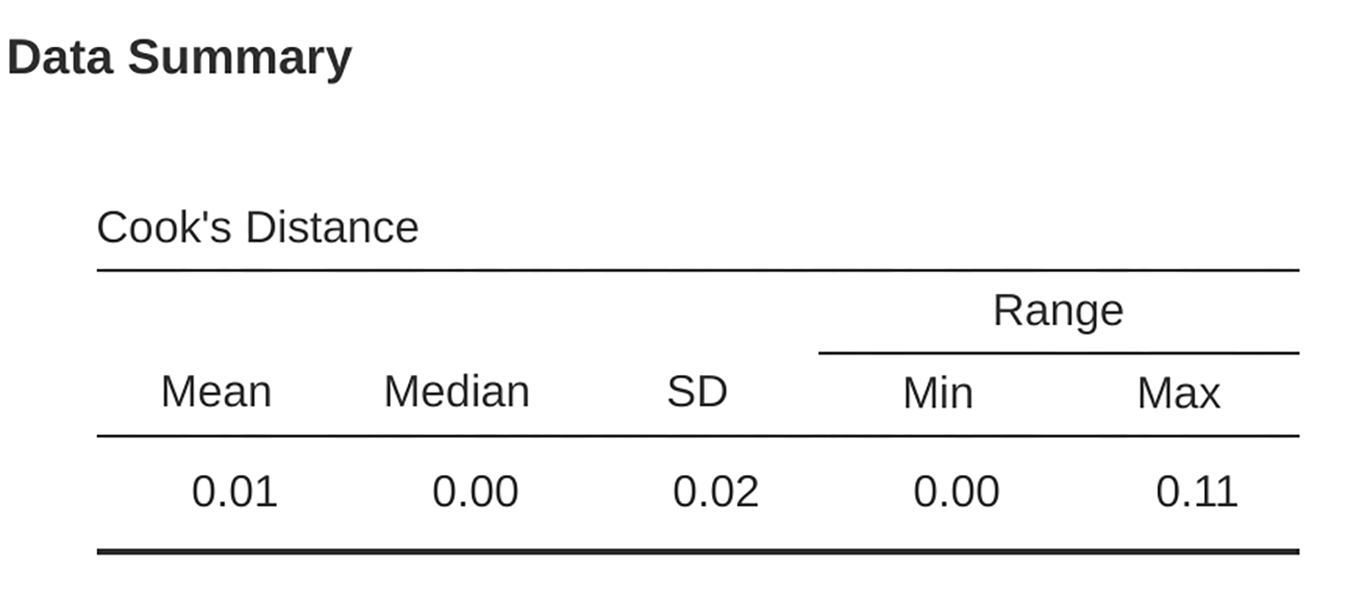
\includegraphics[width=0.8\textwidth,height=\textheight]{images/fig12-27.png} \hfill{}

\caption{\label{fig-fig12-27}jamovi output showing the table for the
Cooks distance statistics}

\end{figure}

You can see that, in this example, the mean Cook's distance value is
\(0.01\), and the range is from \(0.00\) to \(0.11\), so this is some
way off the rule of thumb figure mentioned above that a Cook's distance
greater than 1 is considered large.

An obvious question to ask next is, if you do have large values of
Cook's distance what should you do? As always, there's no hard and fast
rule. Probably the first thing to do is to try running the regression
with the outlier with the greatest Cook's distance\footnote{In jamovi
  you can save the Cook's distance values to the data set, then draw a
  boxplot of the Cook's distance values to identify the specific
  outliers. Or you could use a more powerful regression program such as
  the ``car'' package in R which has more options for advanced
  regression diagnostic analysis.} excluded and see what happens to the
model performance and to the regression coefficients. If they really are
substantially different, it's time to start digging into your data set
and your notes that you no doubt were scribbling as your ran your study.
Try to figure out why the point is so different. If you start to become
convinced that this one data point is badly distorting your results then
you might consider excluding it, but that's less than ideal unless you
have a solid explanation for why this particular case is qualitatively
different from the others and therefore deserves to be handled
separately.

\hypertarget{model-selection}{%
\section{Model selection}\label{model-selection}}

One fairly major problem that remains is the problem of ``model
selection''. That is, if we have a data set that contains several
variables, which ones should we include as predictors, and which ones
should we not include? In other words, we have a problem of
\textbf{variable selection}. In general, model selection is a complex
business but it's made somewhat simpler if we restrict ourselves to the
problem of choosing a subset of the variables that ought to be included
in the model. Nevertheless, I'm not going to try covering even this
reduced topic in a lot of detail. Instead, I'll talk about two broad
principles that you need to think about, and then discuss one concrete
tool that jamovi provides to help you select a subset of variables to
include in your model. First, the two principles:

\begin{itemize}
\item
  It's nice to have an actual substantive basis for your choices. That
  is, in a lot of situations you the researcher have good reasons to
  pick out a smallish number of possible regression models that are of
  theoretical interest. These models will have a sensible interpretation
  in the context of your field. Never discount the importance of this.
  Statistics serves the scientific process, not the other way around.
\item
  To the extent that your choices rely on statistical inference, there
  is a trade off between simplicity and goodness of fit. As you add more
  predictors to the model you make it more complex. Each predictor adds
  a new free parameter (i.e., a new regression coefficient), and each
  new parameter increases the model's capacity to ``absorb'' random
  variations. So the goodness of fit (e.g., \(R^2\)) continues to rise,
  sometimes trivially or by chance, as you add more predictors no matter
  what. If you want your model to be able to generalise well to new
  observations you need to avoid throwing in too many variables.
\end{itemize}

This latter principle is often referred to as \textbf{Ockham's razor}
and is often summarised in terms of the following pithy saying: do not
multiply entities beyond necessity. In this context, it means don't
chuck in a bunch of largely irrelevant predictors just to boost your
\(R^2\). Hmm. Yeah, the original was better.

In any case, what we need is an actual mathematical criterion that will
implement the qualitative principle behind Ockham's razor in the context
of selecting a regression model. As it turns out there are several
possibilities. The one that I'll talk about is the \textbf{Akaike
information criterion} (AIC) (Akaike, 1974) simply because it's
available as an option in jamovi.\footnote{In the context of a linear
  regression model (and ignoring terms that don't depend on the model in
  any way!), the AIC for a model that has \(K\) predictor variables plus
  an intercept is \(AIC=\frac{SS_{res}}{\hat{\sigma}^2}+2K\).}

The smaller the AIC value, the better the model performance. If we
ignore the low level details it's fairly obvious what the AIC does. On
the left we have a term that increases as the model predictions get
worse; on the right we have a term that increases as the model
complexity increases. The best model is the one that fits the data well
(low residuals, left-hand side) using as few predictors as possible (low
K, right-hand side). In short, this is a simple implementation of
Ockham's razor.

AIC can be added to the `Model Fit Measures' output Table when the `AIC'
checkbox is clicked, and a rather clunky way of assessing different
models is seeing if the AIC value is lower if you remove one or more of
the predictors in the regression model. This is the only way currently
implemented in jamovi, but there are alternatives in other more powerful
programmes, such as R. These alternative methods can automate the
process of selectively removing (or adding) predictor variables to find
the best AIC. Although these methods are not implemented in jamovi, I
will mention them briefly below just so you know about them.

\hypertarget{backward-elimination}{%
\subsection{Backward elimination}\label{backward-elimination}}

In backward elimination you start with the complete regression model,
including all possible predictors. Then, at each ``step'' we try all
possible ways of removing one of the variables, and whichever of these
is best (in terms of lowest AIC value) is accepted. This becomes our new
regression model, and we then try all possible deletions from the new
model, again choosing the option with lowest AIC. This process continues
until we end up with a model that has a lower AIC value than any of the
other possible models that you could produce by deleting one of its
predictors.

\hypertarget{forward-selection}{%
\subsection{Forward selection}\label{forward-selection}}

As an alternative, you can also try \textbf{forward selection}. This
time around we start with the smallest possible model as our start
point, and only consider the possible additions to the model. However,
there's one complication. You also need to specify what the largest
possible model you're willing to entertain is.

Although backward and forward selection can lead to the same conclusion,
they don't always.

\hypertarget{a-caveat}{%
\subsection{A caveat}\label{a-caveat}}

Automated variable selection methods are seductive things, especially
when they're bundled up in (fairly) simple functions in powerful
statistical programmes. They provide an element of objectivity to your
model selection, and that's kind of nice. Unfortunately, they're
sometimes used as an excuse for thoughtlessness. No longer do you have
to think carefully about which predictors to add to the model and what
the theoretical basis for their inclusion might be. Everything is solved
by the magic of AIC. And if we start throwing around phrases like
Ockham's razor, well it sounds like everything is wrapped up in a nice
neat little package that no-one can argue with.

Or, perhaps not. Firstly, there's very little agreement on what counts
as an appropriate model selection criterion. When I was taught backward
elimination as an undergraduate, we used \(F\)-tests to do it, because
that was the default method used by the software. I've described using
AIC, and since this is an introductory text that's the only method I've
described, but the AIC is hardly the Word of the Gods of Statistics.
It's an approximation, derived under certain assumptions, and it's
guaranteed to work only for large samples when those assumptions are
met. Alter those assumptions and you get a different criterion, like the
Bayesian Information Criterion (BIC) for instance (also available in
jamovi). Take a different approach again and you get the normalised
maximum likelihood (NML) criterion. Decide that you're a Bayesian and
you get model selection based on posterior odds ratios. Then there are a
bunch of regression specific tools that I haven't mentioned. And so on.
All of these different methods have strengths and weaknesses, and some
are easier to calculate than others (AIC is probably the easiest of the
lot, which might account for its popularity). Almost all of them produce
the same answers when the answer is ``obvious'' but there's a fair
amount of disagreement when the model selection problem becomes hard.

What does this mean in practice? Well, you could go and spend several
years teaching yourself the theory of model selection, learning all the
ins and outs of it so that you could finally decide on what you
personally think the right thing to do is. Speaking as someone who
actually did that, I wouldn't recommend it. You'll probably come out the
other side even more confused than when you started. A better strategy
is to show a bit of common sense. If you're staring at the results of an
automated backwards or forwards selection procedure, and the model that
makes sense is close to having the smallest AIC but is narrowly defeated
by a model that doesn't make any sense, then trust your instincts.
Statistical model selection is an inexact tool, and as I said at the
beginning, interpretability matters.

\hypertarget{comparing-two-regression-models}{%
\subsection{Comparing two regression
models}\label{comparing-two-regression-models}}

An alternative to using automated model selection procedures is for the
researcher to explicitly select two or more regression models to compare
to each other. You can do this in a few different ways, depending on
what research question you're trying to answer. Suppose we want to know
whether or not the amount of sleep that my son got has any relationship
to my grumpiness, over and above what we might expect from the amount of
sleep that I got. We also want to make sure that the day on which we
took the measurement has no influence on the relationship. That is,
we're interested in the relationship between baby.sleep and dani.grump,
and from that perspective dani.sleep and day are nuisance variable or
\textbf{covariates} that we want to control for. In this situation, what
we would like to know is whether dani.grump \textasciitilde{} dani.sleep
+ day + baby .sleep (which I'll call Model 2, or M2) is a better
regression model for these data than dani.grump \textasciitilde{}
dani.sleep + day (which I'll call Model 1, or M1). There are two
different ways we can compare these two models, one based on a model
selection criterion like AIC, and the other based on an explicit
hypothesis test. I'll show you the AIC based approach first because it's
simpler, and follows naturally from discussion in the last section. The
first thing I need to do is actually run the two regressions, note the
AIC for each one, and then select the model with the smaller AIC value
as it is judged to be the better model for these data. Actually, don't
do this just yet. Read on because there is an easy way in jamovi to get
the AIC values for different models included in one table.\footnote{While
  I'm on this topic I should point out that the empirical evidence
  suggests that BIC is a better criterion than AIC. In most simulation
  studies that I've seen, BIC does a much better job of selecting the
  correct model.}

A somewhat different approach to the problem comes out of the hypothesis
testing framework. Suppose you have two regression models, where one of
them (Model 1) contains a subset of the predictors from the other one
(Model 2). That is, Model 2 contains all of the predictors included in
Model 1, plus one or more additional predictors. When this happens we
say that Model 1 is nested within Model 2, or possibly that Model 1 is a
submodel of Model 2. Regardless of the terminology, what this means is
that we can think of Model 1 as a null hypothesis and Model 2 as an
alternative hypothesis. And in fact we can construct an \(F\)-test for
this in a fairly straightforward fashion.\footnote{We can fit both
  models to the data and obtain a residual sum of squares for both
  models. I'll denote these as: \(SS_{res}^{(1)}\) and
  \(SS_{res}^{(2)}\) respectively. The superscripting here just
  indicates which model we're talking about. Then our \(F\) statistic
  is:
  \[F= \frac {\frac {SS _{res}^{(1)} - SS_{res}^{(2)}} {k}}   {\frac{SS_{res}^2} {N-p-1} }\]
  where \(N\) is the number of observations, \(p\) is the number of
  predictors in the full model (not including the intercept), and \(k\)
  is the difference in the number of parameters between the two
  models.\(^d\) The degrees of freedom here are \(k\) and \(N -p-1\).
  Note that it's often more convenient to think about the difference
  between those two \(SS\) values as a sum of squares in its own right.
  That is: \[SS_\Delta=SS_{res}^{(1)}-SS_{res}^{(2)}\] The reason why
  this is helpful is that we can express \(SS_\Delta\) as a measure of
  the extent to which the two models make different predictions about
  the the outcome variable. Specifically:
  \[SS_\Delta=\sum_i{(\hat{y}_i^{(2)}-\hat{y}_i^{(1)})^2}\] where
  \(\hat{y}_{i^{(1)}}\) is the predicted value for \(y_i\) according to
  model \(M_1\) and \(\hat{y}_{i^{(2)}}\) is the predicted value for
  \(y_i\) according to model \(M_2\). --- \(^d\) It's worth noting in
  passing that this same \(F\) statistic can be used to test a much
  broader range of hypotheses than those that I'm mentioning here. Very
  briefly, notice that the nested model \(M_1\) corresponds to the full
  model \(M_2\) when we constrain some of the regression coefficients to
  zero. It is sometimes useful to construct sub-models by placing other
  kinds of constraints on the regression coefficients. For instance,
  maybe two different coefficients might have to sum to zero. You can
  construct hypothesis tests for those kind of constraints too, but it
  is somewhat more complicated and the sampling distribution for \(F\)
  can end up being something known as the non-central
  \(F\)-distribution, which is way beyond the scope of this book! All I
  want to do is alert you to this possibility.}

Okay, so that's the hypothesis test that we use to compare two
regression models to one another. Now, how do we do it in jamovi? The
answer is to use the `Model Builder' option and specify the Model 1
predictors dani.sleep and day in `Block 1' and then add the additional
predictor from Model 2 (baby.sleep) in `Block 2', as in
Figure~\ref{fig-fig12-28}. This shows, in the `Model Comparisons' Table,
that for the comparisons between Model 1 and Model 2,
\(F(1,96) = 0.00\), \(p = 0.954\). Since we have p \textgreater{} .05 we
retain the null hypothesis (M1). This approach to regression, in which
we add all of our covariates into a null model, then add the variables
of interest into an alternative model, and then compare the two models
in a hypothesis testing framework, is often referred to as
\textbf{hierarchical regression}.

We can also use this `Model Comparison' option to display a table that
shows the AIC and BIC for each model, making it easy to compare and
identify which model has the lowest value, as in
Figure~\ref{fig-fig12-28}.

\begin{figure}[H]

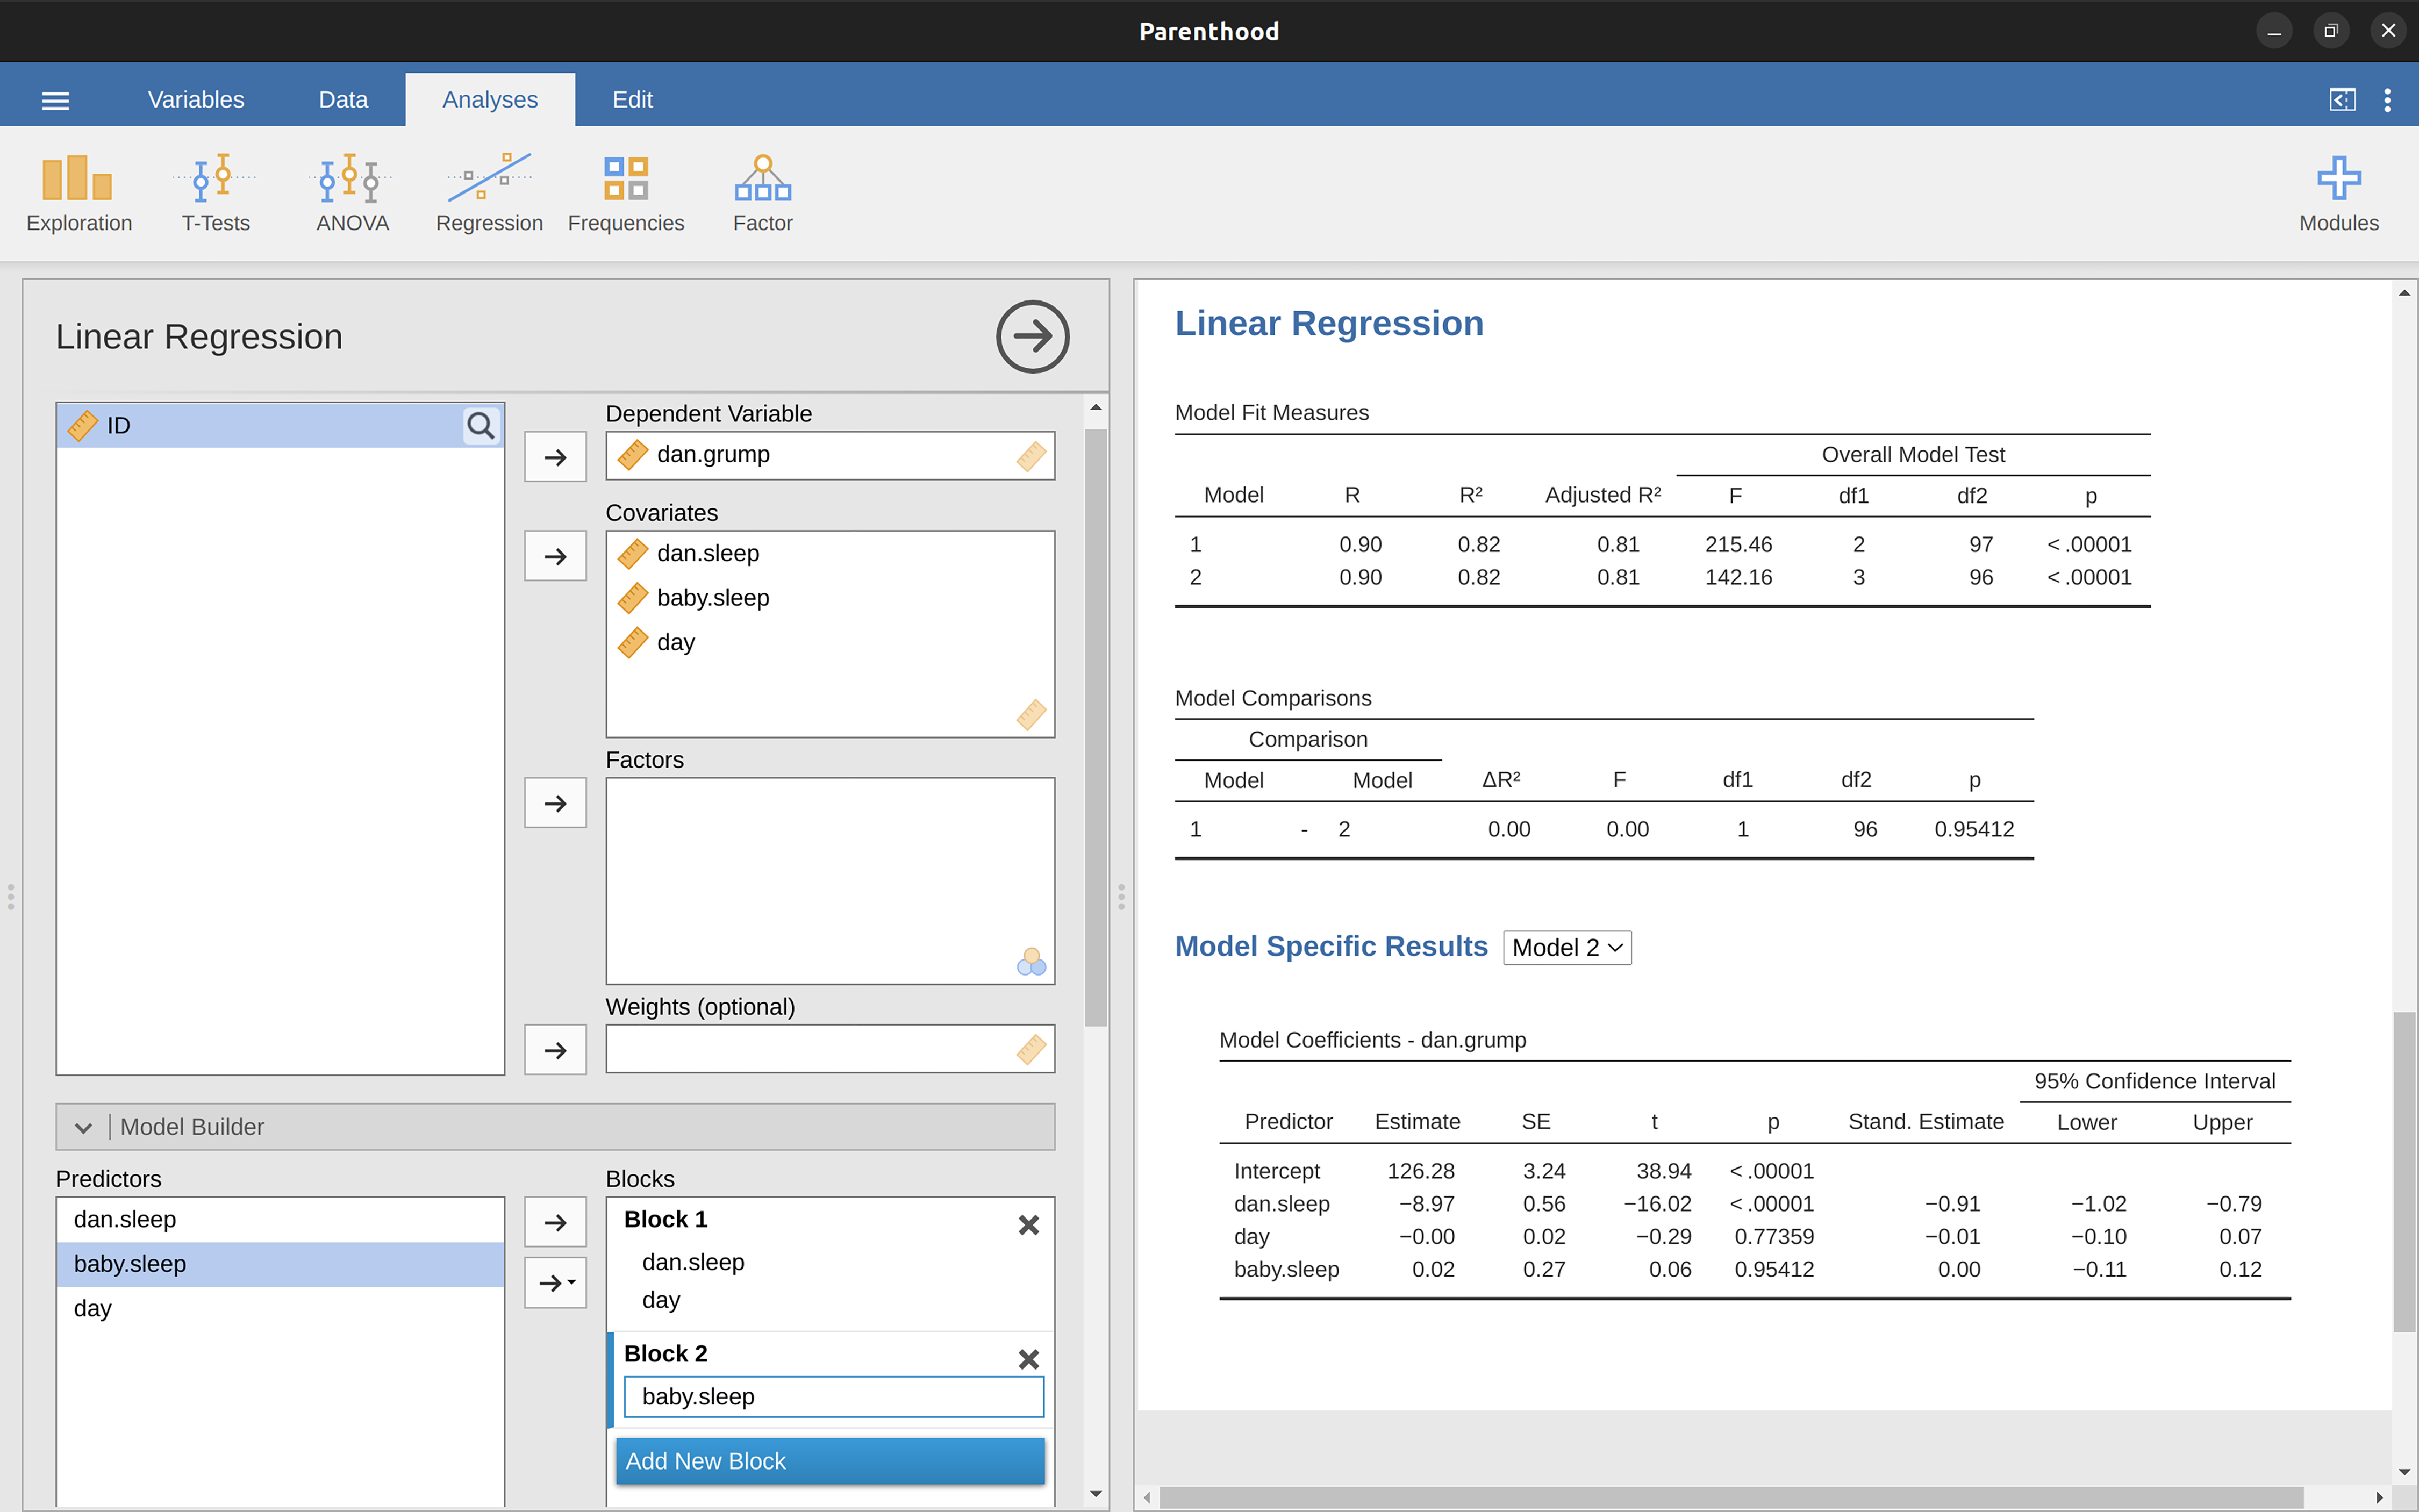
\includegraphics[width=1\textwidth,height=\textheight]{images/fig12-28.png} \hfill{}

\caption{\label{fig-fig12-28}Model comparison in jamovi using the `Model
Builder' option}

\end{figure}

\hypertarget{summary}{%
\section{Summary}\label{summary}}

\begin{itemize}
\tightlist
\item
  Want to know how strong the relationship is between two variables?
  Calculate \protect\hyperlink{correlations}{Correlations}.
\item
  Drawing \protect\hyperlink{scatterplots}{Scatterplots}.
\item
  Basic ideas about
  \protect\hyperlink{what-is-a-linear-regression-model}{What is a linear
  regression model?} and
  \protect\hyperlink{estimating-a-linear-regression-model}{Estimating a
  linear regression model}.
\item
  \protect\hyperlink{multiple-linear-regression}{Multiple linear
  regression}.
\item
  \protect\hyperlink{quantifying-the-fit-of-the-regression-model}{Quantifying
  the fit of the regression model} using \(R^2\).
\item
  \protect\hyperlink{hypothesis-tests-for-regression-models}{Hypothesis
  tests for regression models}.
\item
  In \protect\hyperlink{regarding-regression-coefficients}{Regarding
  regression coefficients} we talked about calculating
  \protect\hyperlink{confidence-intervals-for-the-coefficients}{Confidence
  intervals for the coefficients} and
  \protect\hyperlink{calculating-standardised-regression-coefficients}{Calculating
  standardised regression coefficients}.
\item
  The \protect\hyperlink{assumptions-of-regression}{Assumptions of
  regression} and \protect\hyperlink{sec-Model-checking}{Model
  checking}.
\item
  Regression \protect\hyperlink{model-selection}{Model selection}.
\end{itemize}

\hypertarget{refs}{}
\begin{CSLReferences}{1}{0}
\leavevmode\vadjust pre{\hypertarget{ref-Akaike1974}{}}%
Akaike, H. (1974). A new look at the statistical model identification.
\emph{IEEE Transactions on Automatic Control}, \emph{19}, 716--723.
\url{https://doi.org/10.1109/TAC.1974.1100705}

\leavevmode\vadjust pre{\hypertarget{ref-Anscombe1973}{}}%
Anscombe, F. J. (1973). Graphs in statistical analysis. \emph{American
Statistician}, \emph{27}, 17--21.
\url{https://doi.org/10.1080/00031305.1973.10478966}

\leavevmode\vadjust pre{\hypertarget{ref-Fox2011}{}}%
Fox, J., \& Weisberg, S. (2011). \emph{An {R} companion to applied
regression} (2nd ed.). Sage.

\end{CSLReferences}


\backmatter

\printendnotes
\newpage

\chapter{About the team}

Alessandra Tosi was the managing editor for this book.

Tricia de Souza and Adèle Kreager proof-read this manuscript.

The cover was designed by Jeevanjot Kaur Nagpal, and produced in InDesign using the Fontin and Calibri fonts.

David Foxcroft and Cameron Craig produced the printed PDF editions. 

David Foxcroft produced the HTML edition.

Raegan Allen was in charge of marketing.

This book was peer-reviewed by two referees. Experts in their field, these readers give their time freely to help ensure the academic rigour of our books. We are grateful for their generous and invaluable contributions.

\newpage


%\printindex
%back cover
%\includepdf[fitpaper=true,pages=-]{images/backcover8x10}
%\pagenumbering{gobble} 

\end{document}
